%
% Master LaTeX document.
%
% Define document type.
\documentclass[11pt,a4paper,english,titlepage]{article}

% Include packages.
\usepackage{cite}
\usepackage{gtupgrade}
\usepackage{footmisc} % for footnote references on different places

% Document information.
\def\doctitle{Global Trigger firmware Specification for MP7 platform for Upgrade Phase I}
\def\docauthor{Herbert Bergauer, Babak Rahbaran, Johannes Wittmann}
\def\docdate{\today}

% Custom commands => see ../utils/latex/gtupgrade.sty.

% HB 2022-03-01: Get versions from file - edit file for new versions
\newcommand{\versiongt}{v1.26.0 }
\newcommand{\versionframe}{v1.4.2 }
\newcommand{\versiongtl}{v1.20.0 }
\newcommand{\versionfdl}{v1.4.1 }
\newcommand{\gitbranch}{https://github.com/cms-l1-globaltrigger/mp7_ugt_legacy/blob/cicada_topo}


% Begin document structure.
\begin{document}

    % Title page.
    \doctitlepage{}

    % Document revision history.
    \section*{Revision History}
\label{sec:revision_history}

\begin{longtable}{|c|p{.65\columnwidth}|c|}
\hline
Doc Rev & Description of Change & Revision Date\\
\hline
\hline
\endhead
2.29 & Updated text for cuts on muon index bits (\ref{sec:gtl:muon_data} and \ref{sec:gtl:calc_obj_cuts}) & 2023/02/20\\
2.28 & Added tables (\ref{table:app:sum_opt_links}) and (\ref{table:app:sum_opt_links2}), removed figure "Optical link inputs to Global Trigger". Removed chapter "GTH I/Os" from "Appendices" & 2023/02/09\\
2.27 & Added table for muon charge bits(\ref{tab:gtl:muon_charge_bits}). & 2023/01/16\\
2.26 & Updated figure (\ref{fig:gtl:tme_gtl}), references and text (\ref{sec:fw:gt_system} and \ref{sec:gtl:implementation_firmware_gtl}). Renumbered "Revision History". & 2023/01/10\\
2.25 & Updated text "LUTs for 1/deltaR**2 used in mass over deltaR calculations" (\ref{sec:gtl:calc_luts_inverse_deltaR}). & 2023/01/09\\
2.24 & Cleaned up text and layout. & 2022/12/15\\
2.23 & Added chapter "Handling of timing errors in synthesis" (\ref{sec:app:synth_timing_errors}). & 2022/12/01\\
2.22 & Cleaned up (used "textquotesingle"). & 2022/11/30\\
2.21 & Updated "Configuration of GTHs" (\ref{sec:app:gth_conf_table}). & 2022/11/24\\
2.20 & Inserted chapter "GTH I/Os" to "Appendices" (\ref{sec:app:gth_io}). & 2022/10/12\\
2.19 & Added table "Firmware versions" (\ref{tab:fw:versions}). & 2022/09/27\\
2.18 & Updated "Appendices" (\ref{sec:app:app}). & 2022/09/26\\
2.17 & Updated text in "LUTs for 1/$\Delta$$R^2$" (\ref{sec:gtl:calc_luts_corr_cuts}), added new chapter "Muon shower bits" (\ref{sec:gtl:muon_shower_bits}). & 2022/09/13\\
2.16 & Updated text for \finor-mask and veto-mask (\ref{sec:fdl:finor_masks} and \ref{sec:fdl:veto_masks}). Updated \href{\gitbranch/tree/master/doc/mp7_ugt_firmware_specification/src/latex/content/versions.tex}{\texttt{versions.tex}}. & 2022/09/09\\
2.15 & Updated text for "fractional prescale", reset prescaler with "start" (\ref{sec:fdl:pre_scalers}). & 2022/08/17\\
2.14 & Updated text for "fractional prescale" values (\ref{sec:fdl:pre_scalers}). & 2022/07/11\\
2.13 & Inserted "Description of tests" to "Appendices" (\ref{sec:app:app_e}). & 2022/03/25\\
2.12 & Cleaned up text and tables in section "Framework" (\ref{sec:framework:framework}). Changed links to firmware modules (git branch name set in versions.tex). & 2022/03/23\\
2.11 & Added "Configuration of optical input links" and "Configuration of links to AMC13 (readout)" to "Appendices" (\ref{sec:app:app_b} and \ref{sec:app:app_c}). & 2022/02/28\\
2.10 & Inserted "Appendices" (\ref{sec:app:app}) and added references. & 2022/02/25\\
2.9 & Inserted "Simulation and build of firmware" and "Testing firmware" (\ref{sec:fw:sim_build_firmware} and \ref{sec:fw:testing_firmware}). & 2022/02/15\\
2.8.1 & Bug fixed in labels. Updated labels. & 2022/02/14\\
2.8 & Inserted "Implementation in firmware" for top-of-hierarchy of VHDL code (\ref{sec:fw:implementation_firmware}). Updated labels. & 2022/02/11\\
2.7 & Updated text of section "Implementation in firmware" for Framework (\ref{sec:framework:implementation_firmware}), GTL (\ref{sec:gtl:implementation_firmware_gtl}) and FDL (\ref{sec:fdl:implementation_firmware}). & 2022/02/10\\
2.6 & Inserted references and updated text in \ref{sec:fw:dir_struct_gt_fw}. & 2022/02/09\\
2.5 & Updated text in "Implementation in firmware" (\ref{sec:gtl:implementation_firmware_gtl}). & 2022/01/10\\
2.4.1 & Bug fixed in definition of calo eta ranges (\ref{sec:gtl:calorimeter_data}). & 2021/11/30\\
2.4 & Updated data structure for jets with DISP bit (\ref{sec:gtl:gct_optical_interfaces}). & 2021/11/17\\
2.3 & Inserted "Calculation of look-up-tables (LUTs) for correlation cuts" (\ref{sec:gtl:calc_luts_corr_cuts}). & 2021/11/10\\
2.2 & Removed "VHDL-Templates for VHDL-Producer". & 2021/09/24\\
2.1 & Updated (and renamed) description of "Invariant mass over delta R calculation" (see \ref{sec:gtl:inv_mass_div_dr_calculation}). & 2021/09/14\\
2.0 & New structure of document for firmware versions 1.12.x and higher. & 2021/02/10\\
1.53.1 & Fixed typo in section "Invariant mass calculation for three objects" \ref{sec:gtl:inv_mass_3_obj_calculation}. & 2020/12/03\\
1.53 & Updated text in section "VHDL-Templates for VHDL-Producer". & 2020/09/31\\
1.52 & Inserted links to VHDL modules. & 2020/09/18\\
1.51 & Updated text in section "Correlation conditions" \ref{sec:gtl:correlation_conditions}. Description is for v1.10.0 of Global Trigger Logic. & 2020/09/17\\
1.50 & Inserted description of "Invariant mass divided by delta R calculation" (see \ref{sec:gtl:inv_mass_div_dr_calculation}). & 2020/09/10\\
1.49.1 & Fixed typo (unconstrained pt). & 2020/09/09\\
1.49 & Inserted text for new muon structure in sections \ref{sec:gtl:gmt_optical_interfaces}, \ref{sec:gtl:muon_data} and \ref{sec:gtl:correlation_condition_modules}. Added subsections in section "VHDL-Templates for VHDL-Producer" & 2020/08/04\\
1.48 & Additional text in section for calo calo overlap remover condition module. & 2020/05/25\\
1.47 & Inserted text in section Calorimeter Overlap Remover conditions and Calo Calo Overlap Remover Correlation conditions. & 2020/04/16\\
1.46 & Updated text in sections Calorimeter conditions, Muon conditions and Correlation conditions for changes which have been done for GTL VHDL version 1.8.0 (module names without version number, "five eta cuts"). & 2019/08/13\\
1.45 & Inserted "Asymmetry" and "Centrality" of "Energy sums" (GTL VHDL version 1.6.0). Therefore updated sections \ref{sec:gtl:ugtl_interface}, \ref{sec:gtl:gct_optical_interfaces},
\ref{sec:gtl:esums_conditions} added section "Centrality condition" \ref{sec:gtl:centrality_cond} and updated Table \ref{tab:framework:tab_configuration_optical_conn} & 2018/08/13\\
1.44 & Updated text in section "Global Trigger Logic" (\ref{sec:gtl:global_trigger_logic}) according to firmware version v1.5.0 of gtl\_module.vhd. & 2018/02/21\\
1.43 & Updated text in section "Framework" (\ref{sec:framework:framework}) according to firmware version v1.2.3 of frame.vhd. & 2018/01/19\\
1.42 & New "icons" ET$_{miss}^{HF}$ and HT$_{miss}^{HF}$ in Table~\ref{tab:framework:tab_configuration_optical_conn} and Section \ref{sec:gtl:global_trigger_logic}. Updated glossary. & 2016/11/11\\
1.41 & Updated table "\ufdl register map" (\ref{tab:fdl:ufdl_register_map}) and section "Register map" (\ref{sec:fdl:reg_map}). Moved "List of Tables" and "List of Figures" to the end of document.
Inserted link to "Scales for inputs to $\mu$GT" (\ref{sec:gtl:implementation_firmware_gtl}). Moved section "Software reset" to section "Framework" as subsection (\ref{sec:framework:software_reset}).
Removed empty sections "IPBus", "Firmware Configuration" and "Bibliography". & 2016/11/03\\
1.40 & Updated sections "Calo-Layer2 optical interfaces" (\ref{sec:gtl:gct_optical_interfaces}) and "Energy sum quantities conditions" (\ref{sec:gtl:esums_conditions})
for towercount trigger bits. Inserted section "Towercount condition" (\ref{sec:gtl:towercount_cond}). & 2016/10/25\\
1.39 & Updated section "Calo-Layer2 optical interfaces" (\ref{sec:gtl:gct_optical_interfaces}) for new energy sum quantities and minimum bias trigger bits.
Updated sections "Firmware" (\ref{sec:fw:fw}), "Framework" (\ref{sec:framework:framework}) and "Final Desicion Logic" (\ref{sec:fdl:ufdl}). & 2016/06/09\\
1.38 & Updated Text in section "Muon Muon Correlation condition module". & 2016/01/15\\
1.37 & Removed "Double objects requirements condition with spatial correlation", because not used anymore in the future, replaced by Correlation conditions. & 2016/01/08\\
1.36 & Minor changes in text and updated Figure \ref{fig:gtl:gtl_pipeline}. & 2016/01/08\\
1.35 & Changed colour in Figure \ref{fig:gtl:phi_windows_comparator} and updated text for correlation conditions (see section~\ref{sec:gtl:correlation_conditions}. & 2016/01/07\\
1.34 & Updated Figures \ref{fig:gtl:gtl_pipeline} and \ref{fig:gtl:tme_gtl} and text in calo calo correlation condition module. & 2015/12/21\\
1.33 & Inserted drawing of VHDL structure of cuts for correlation conditions (see Figure~\ref{fig:gtl:scheme_vhdl_cuts_correllation_condition}). & 2015/11/18\\
1.32 & Updated muon $\eta$ ranges (Table~\ref{tab:gtl:muon_eta_scale}) and inserted correlation conditions.
Created scheme for conversion of calorimeter $\eta$ and $\varphi$ to muon scale for calo-muon-correlation conditions. & 2015/11/17\\
1.31 & Added Text in sections calo comparator module and muon comparator module. & 2015/10/08\\
1.30 & Updated Text in section "Final Desicion Logic" (\ref{sec:fdl:ufdl}). & 2015/10/06\\
1.29 & Updated Figure \ref{fig:fdl:mFDL_firmware} and Tables \ref{tab:fdl:ufdl_register_map}. Remaned
section "Calorimeter conditions module - version 2" to "Calorimeter conditions module - version 3", section "Muon conditions module" to "Muon conditions module - version 2"
and section "Muon comparators module" to "Muon comparators module - version 2". & 2015/10/02\\
1.28 & Updated text and tables of $\eta$ ranges for Calorimeter objects (see \ref{sec:gtl:calorimeter_data}). & 2015/09/22\\
1.27 & Renewed Figures in GTL and FDL (see Figure~\ref{fig:gtl:mGTL_firmware}, \ref{fig:gtl:tme_gtl} and \ref{fig:gtl:gtl_pipeline})
and FDL(see Figure~\ref{fig:fdl:mFDL_firmware} and \ref{fig:fdl:mFDL_pipeline}). Added register bits description of FDL Register map (see section~\ref{sec:fdl:reg_map}). & 2015/09/16\\
1.26 & Updated text, tables and listings of section "VHDL-Templates for VHDL-Producer". & 2015/09/15\\
1.25 & Corrected calculation of muon $\eta$ step width (see \ref{sec:gtl:muon_data}). & 2015/09/10\\
1.24 & Edited text in Table \ref{tab:gtl:muon_lut_qual}. & 2015/08/28\\
1.23 & Updated definition of $\eta$ ranges for Calorimeter objects and Muon objects. & 2015/08/20\\
1.22 & Added section Calo Muon Correlation condition. & 2015/08/19\\
1.21 & Added section "Register map" (\ref{sec:fdl:reg_map}) for \ufdl. & 2015/06/26\\
1.20 & Updated figures (\ref{fig:gtl:mGTL_firmware}, \ref{fig:gtl:tme_gtl} and \ref{fig:gtl:gtl_pipeline}) for GTL and edited section
"Correlation conditions" (see \ref{sec:gtl:correlation_conditions}). & 2015/05/08\\
1.19 & Added tables for calorimeter isolation-bits and for muon quality- and isolation-bits definition (\ref{tab:gtl:eg_tau_iso_bits}, \ref{tab:gtl:muon_quality_bits} and \ref{tab:gtl:muon_iso_bits}).
Edited section glossary and acronyms. & 2015/05/07\\
1.18 & Added text for "Energy sum conditions" (\ref{sec:gtl:esums_conditions}) and updated chapters for "Calorimeter conditions" for version 2. Inserted isolation bits for \egamma and tau objects
(\ref{sec:gtl:calorimeter_data}). & 2015/05/06\\
1.17 & Minor changes "Demux Lane Data" (see \ref{sec:framework:demux_lane_data}) and "Muon data" (see \ref{sec:gtl:muon_data}). & 2014/11/06\\
1.16 & Edited Section "Energy sum quantities conditions" (see \ref{sec:gtl:esums_conditions}). & 2014/10/08\\
1.15 & Added sections "Configuration of optical connections" (\ref{sec:framework:sec_configuration_optical_conn}), "Demux Lane Data" (\ref{sec:framework:demux_lane_data})
and "Lane Mapping Process" (\ref{sec:framework:lmp}) to framework. Removed tables of optical interfaces from gtl and referenced to tables in framework. & 2014/10/07\\
1.14 & Minor changes in "Calorimeter conditions" and "Muon conditions" . & 2014/07/01\\
1.13 & Updated with minor changes in "Muon conditions". & 2014/06/17\\
1.12.1 & Fixed bug in Figure \ref{fig:gtl:phi_windows_comparator}. & 2014/04/30\\
1.12 & Updated section "Muon conditions". & 2014/04/22\\
1.11 & Removed section "Muon charge module" and added new section "Muon charge correlation module" (see \ref{sec:gtl:muon_charge_correlation_module}).
Edited text in section and subsections "Muon conditions definition". & 2014/04/15\\
1.10 & Changed Figure~\ref{fig:gtl:phi_windows_comparator} and minor changes in text for anti-clockwise behaviour in $\varphi$. & 2014/04/04\\
1.9 & Added definition for "calorimeter conditions over bx", see section. & 2014/03/12\\
1.8 & Changed text of condition description in subsections Calo conditions definition and Muon conditions definition. & 2014/02/12\\
1.7 & Updated calorimeter data structure in \ref{sec:gtl:gct_optical_interfaces}. & 2013/12/03\\
1.6 & Updated muon data structure in \ref{sec:gtl:gmt_optical_interfaces} & 2013/12/02\\
1.5 & Moved decription of VHDL templates for TME to "VHDL-Templates for VHDL-Producer". & 2013/11/18\\
1.4 & Subsection~\ref{sec:gtl:optical_interfaces} added to section \ref{sec:gtl:global_trigger_logic}. & 2013/11/11\\
1.3 & GTL and FDL firmware implemented for new data structure (GTL firmware version v1.0.0 [fix part of GTL], FDL firmware version v1.0.0) & 2013/11/06\\
1.2 & New framework implementation based on new object types definition. Additionally, the ROP is implemented based on production requirements. & 2013/10/13\\
1.1 & First framework implementation and ROP. & 2012/07/01\\
1.0 & Document created. & 2012/02/22\\
\hline
\end{longtable}

\clearpage{}


    % Table of contents.
    \doctoc{}

    % Document content.
    \section{Global Trigger System overview}\label{sec:fw:gt_system}

The Global Trigger System is based on MicroTCA technology and 10 Gbps optical links. A set of 6 MP7 boards (for MP7 documentation see~\cite{MP7}, for MP7 firmware see~\cite{MP7 firmware}) with a FPGA of the powerful Xilinx Virtex-7 family (XC7VX690TFFG1927-2, see~\cite{Virtex7}) is available. The Global Trigger firmware is implemented on these FPGAs. Every FPGA contains a part of the VHDL representation of a L1 Menu, the partitioning is done by VHDL Producer tool. The trigger decision of every MP7 board is collected on an AMC502 board to generate the "final OR" signal which triggers the readout of the detector.

\section{Firmware overview}\label{sec:fw:fw}
The figure \ref{fig:mgt} shows the architecture of \ugt payload. It consists of framework and the algorithm logic which consists of the following modules:
\begin{enumerate}
\item Global Trigger Logic Data Mapping
\item \ugtl
\item \ufdl
\end{enumerate}

The output mux (part of framework) collects data for read-out record which are send via MP7 read-out to AMC13.

The IPBus system allows the control of hardware via a ‘virtual bus’, using a standard IP-over-gigabit-Ethernet network connection.
\begin{figure}[h!]
   \centering
    \includegraphics[width=1.0\textwidth]{figures/mGT_payload}
    \caption{\ugt payload}\label{fig:mgt}
 \end{figure}

\subsection{Firmware versions}\label{sec:fw:fw_version}

This firmware description is based on following versions:
% \begin{itemize}
% \item Framework: \versionframe
% \item Global Trigger Logic: \versiongtl
% \item Final Decision Logic: \versionfdl
% \end{itemize}

\begin{table}[ht]
\caption{Firmware versions}
\vspace{5mm}
\centering
\begin{tabular}{|l|l|}\hline
\textbf{Entity}& \textbf{Version}\\\hline\hline
Global Trigger firmware & \versiongt\\\hline
Framework & \versionframe\\\hline
Global Trigger Logic & \versiongtl\\\hline
Final Decision Logic & \versionfdl\\\hline
\end{tabular}
\label{tab:fw:versions}
\end{table}

\subsection{Directory structure of Global Trigger firmware} \label{sec:fw:dir_struct_gt_fw}

In Global Trigger repository all files for building firmware are in directory \href{\gitbranch/firmware}{\texttt{\textquotesingle firmware\textquotesingle}} with subdirectories for synthesis configuration files (\href{\gitbranch/firmware/cfg}{\texttt{\textquotesingle cfg\textquotesingle }} and \href{\gitbranch/firmware/ucf}{\texttt{\textquotesingle ucf\textquotesingle }}), for VHDL source files (\href{\gitbranch/firmware/hdl}{\texttt{\textquotesingle hdl\textquotesingle }}), for memory files build from IPs (\href{\gitbranch/firmware/ngc}{\texttt{\textquotesingle ngc\textquotesingle }}) and simulation files (\href{\gitbranch/firmware/sim}{\texttt{\textquotesingle sim\textquotesingle }}).\\
All defintions for VHDL code are in \href{\gitbranch/firmware/hdl/packages}{\texttt{\textquotesingle hdl/packages\textquotesingle }}, VHDL source files representing Global Trigger firmware are in \href{\gitbranch/firmware/hdl/payload}{\texttt{\textquotesingle hdl/payload\textquotesingle }} with subdirectories (for \href{\gitbranch/firmware/hdl/payload/gtl}{\texttt{\textquotesingle gtl\textquotesingle }}, \href{\gitbranch/firmware/hdl/payload/fdl}{\texttt{\textquotesingle fdl\textquotesingle }},  \href{\gitbranch/firmware/hdl/payload/frame}{\texttt{\textquotesingle frame\textquotesingle }} and \href{\gitbranch/firmware/hdl/payload/ipbus}{\texttt{\textquotesingle ipbus\textquotesingle }}).

\subsubsection{Implementation in firmware}
\label{sec:fw:implementation_firmware}

Top-of-hierarchy of VHDL code is \href{\gitbranch/firmware/hdl/payload/mp7\_payload.vhd}{\texttt{\textquotesingle mp7\_payload.vhd\textquotesingle }}.

Listing~\ref{lst:fw:mp7_payload_vhd} contains the entity-declaration of the top-of-hierarchy file.

\lstinputlisting[label=lst:fw:mp7_payload_vhd,language=VHDL,caption=Entity declaration of \texttt{mp7\_payload.vhd}]{interfaces/mp7_payload.vhd}

All the declarations for arrays ("type"), parameters ("constant") and look-up-tables ("constant") used in modules are available in \href{\gitbranch/firmware/hdl/packages/gtl\_pkg.vhd}{\texttt{\textquotesingle gtl\_pkg.vhd\textquotesingle }} package-file.

\medskip
\begin{table}
\footnotesize
\caption{Explanation of Listing~\ref{lst:fw:mp7_payload_vhd}}
\vspace{5mm}
\centering
\begin{tabular}{l p{.7\columnwidth}}
\toprule
{Item} & {Explanation}\\
\midrule
\verb|clk| & IPBus clock input.\\
\verb|rst| & IPBus reset input.\\
\verb|ipb_in| & IPBus data input.\\
\verb|ipb_out| & IPBus data output.\\
\verb|clk_payload| & clock inputs [clk\_payload(0)=lhc\_clock].\\
\verb|rst_payload| & reset inputs.\\
\verb|clk_p| & clock 240MHz.\\
\verb|rst_loc| & not used.\\
\verb|clken_loc| & not used.\\
\verb|ctrs| & TTC signals input.\\
\verb|l1a| & L1A signal input.\\
\verb|bc0| & bunch counter reset output.\\
\verb|d| & data input (from optical links).\\
\verb|q| & data output (to optical links).\\
\verb|gpio| & signal outputs to mezzanine board.\\
\verb|gpio_en| & enable (signal) outputs to mezzanine board.\\
\bottomrule
\end{tabular}
\label{tab:gtl:explanation_mp7_payload_vhd}
\end{table}

\clearpage

\subsubsection{Simulation and build of firmware}
\label{sec:fw:sim_build_firmware}

In document \href{\gitbranch/README.md}{\texttt{\textquotesingle README.md\textquotesingle }} one can find instructions for setting up simulation and build environments. For simulation and building of firmware access rights to GitLab (MP7 firmware) are mandatory.

\subsubsection{Testing firmware}
\label{sec:fw:testing_firmware}

Testing of firmware in hardware at CMS P5 (see \ref{sec:app:app_e}) is done with script "multiboard\_function\_test" ("tdf run\ multiboard\_function\_test -h"). Therefore a XML file of the L1Menu and a test vector file must be available at the crate. The firmware of the L1Menu which should be tested must be loaded into the 6 MP7 boards before testing ("tdf run uploadfw\_gt -h"). For checking crate status execute "tdf run crate\_status".\\
This testing is restricted to persons with access to \ugt crates at P5.

\clearpage

    \section{Framework}\label{sec:framework:framework}

This description is for version \versionframe of Framework.\\

\textbf{Remark:}\\
with frame v1.2.3 "Delay Manager" (\texttt{\textquotesingle dm.vhd\textquotesingle }) and "Data Source Multiplexer" (\texttt{\textquotesingle dsmux.vhd\textquotesingle }) are removed because these features were never used in production system, only for tests.
Simmem data not used anymore, because of removed dsmux.
The reason of removing is to get more available resources.\\

Data from the GTH interfaces are demultiplexed (from 240 MHz clock domain to LHC clock domain, see Demux Lane Data \ref{sec:framework:demux_lane_data}) and mapped to objects structure in Lane Mapping Process (LMP) for \ugtl input and SPY I memory.

\subsection{Implementation in firmware}
\label{sec:framework:implementation_firmware}

Listing~\ref{lst:framework:frame_vhd} contains the entity-declaration of \href{\gitbranch/firmware/hdl/payload/frame.vhd}{\texttt{\textquotesingle frame.vhd\textquotesingle }}.\\

\lstinputlisting[label=lst:framework:frame_vhd,language=VHDL,caption=Entity declaration of \texttt{frame.vhd}]{interfaces/frame.vhd}

\clearpage

\medskip
\begin{table}
\footnotesize
\caption{Explanation of Listing~\ref{lst:framework:frame_vhd}}
\vspace{5mm}
\centering
\begin{tabular}{l p{.7\columnwidth}}
\toprule
{Item} & {Explanation}\\
\midrule
\verb|NR_LANES| & number of used optical links.\\
\verb|ipb_clk| & IPBus clock (input).\\
\verb|ipb_rst| & IPBus reset (input).\\
\verb|ipb_in| & IPBus data (input).\\
\verb|ipb_out| & IPBus data (output).\\
\verb|ctrs| & TTC control signals (input).\\
\verb|clk240| & clock (input) 240 MHz.\\
\verb|lhc_clk| & clock (input) (LHC clock).\\
\verb|lhc_rst_o| & reset (output).\\
\verb|bc0| & TTC BGo bunch counter reset (input).\\
\verb|ec0| & TTC BGo event counter reset (input).\\
\verb|oc0| & TTC BGo orbit counter reset (input).\\
\verb|start| & TTC BGo start (input).\\
\verb|l1a| & L1 access signal (input).\\
\verb|bcres_d| & delayed bunch counter reset (output).\\
\verb|bcres_d_FDL| & delayed bunch counter reset (output) fot \ufdl.\\
\verb|start_lumisection| & begin of lumisection (output).\\
\verb|lane_data_in| & data from GTHs (optical links) (input) (240MHz domain).\\
\verb|lane_data_out| & data to GTHs (optical links) (output) (240MHz domain).\\
\verb|lhc_data_2_gtl_o| & data to \ugtl (output) (40MHz domain).\\
\verb|prescale_factor_set_in| & prescale factor set data (input).\\
\verb|algo_after_gtLogic_rop| & algos after \ugtl (input).\\
\verb|algo_after_bxomask_rop| & algos after BX mask (input).\\
\verb|algo_after_prescaler_rop| & algos after prescaler (input).\\
\verb|local_finor_rop| & local FINOR (input).\\
\verb|local_veto_rop| & local VETO (input).\\
\verb|finor_rop| & FINOR (input).\\
\verb|local_finor_with_veto_2_spy2| & local FINOR with VETO to spy mem (input).\\
\bottomrule
\end{tabular}
\label{tab:framework:explanation_frame_vhd}
\end{table}

\clearpage

\subsection{Main parts}

The top-of-hierarchy module of framework (\href{\gitbranch/firmware/hdl/payload/frame.vhd}{\texttt{\textquotesingle frame.vhd\textquotesingle }}) contains
\begin {itemize}
\item demultiplexer of lane data
\item lane mapping
\item spy memories
\item timer counter manager
\item register
\end {itemize}

\subsubsection{Configuration of optical connections} \label{sec:framework:sec_configuration_optical_conn}
The configuration of the optical connections from GMT, Calo-Layer2 and External conditions is done as described in Table~\ref{tab:framework:tab_configuration_optical_conn}, where frame means 32 bits data in a 240 MHz domain.

\begin{table}
\caption{Configuration of optical connections}
\vspace{5mm}
\centering
\begin{tabular}{c|m{.13\columnwidth}|m{.13\columnwidth}|m{.13\columnwidth}|m{.13\columnwidth}|m{.13\columnwidth}|m{.13\columnwidth}|}
\cline{2-7}
 & \multicolumn{6}{c|}{\textbf{frame}} \\\hline
\multicolumn{1}{|c|}{\textbf{link}} & \makebox[.13\columnwidth][c]{\textbf{0}} & \makebox[.13\columnwidth][c]{\textbf{1}} & \makebox[.13\columnwidth][c]{\textbf{2}} & \makebox[.13\columnwidth][c]{\textbf{3}} & \makebox[.13\columnwidth][c]{\textbf{4}} &\makebox[.13\columnwidth][c]{\textbf{5}} \\\hline\hline
\multicolumn{1}{|c|}{0} & reserved & reserved & muon obj. 0 [0..31] & muon obj. 0 [32..63] & muon obj. 1 [0..31] & muon obj. 1 [32..63]\\\hline
\multicolumn{1}{|c|}{1} & reserved & reserved & muon obj. 2 [0..31] & muon obj. 2 [32..63] & muon obj. 3 [0..31] & muon obj. 3 [32..63]\\\hline
\multicolumn{1}{|c|}{2} & reserved & reserved & muon obj. 4 [0..31] & muon obj. 4 [32..63] & muon obj. 5 [0..31] & muon obj. 5 [32..63]\\\hline
\multicolumn{1}{|c|}{3} & reserved & reserved & muon obj. 6 [0..31] & muon obj. 6 [32..63] & muon obj. 7 [0..31] & muon obj. 7 [32..63]\\\hline
\multicolumn{1}{|c|}{4} & \egamma obj. 0 & \egamma obj. 1 & \egamma obj. 2 & \egamma obj. 3 & \egamma obj. 4 & \egamma obj. 5 \\\hline
\multicolumn{1}{|c|}{5} & \egamma obj. 6 & \egamma obj. 7 & \egamma obj. 8 & \egamma obj. 9 & \egamma obj. 10 & \egamma obj. 11 \\\hline
\multicolumn{1}{|c|}{6} & jet obj. 0 & jet obj. 1 & jet obj. 2 & jet obj. 3 & jet obj. 4 & jet obj. 5 \\\hline
\multicolumn{1}{|c|}{7} & jet obj. 6 & jet obj. 7 & jet obj. 8 & jet obj. 9 & jet obj. 10 & jet obj. 11 \\\hline
\multicolumn{1}{|c|}{8} & tau obj. 0 & tau obj. 1 & tau obj. 2 & tau obj. 3 & tau obj. 4 & tau obj. 5 \\\hline
\multicolumn{1}{|c|}{9} & tau obj. 6 & tau obj. 7 & tau obj. 8 & tau obj. 9 & tau obj. 10 & tau obj. 11 \\\hline
\multicolumn{1}{|c|}{\multirow{3}{*}{10}} &
\multicolumn{1}{l|}{\ett} & \htt & \etm & \htm & ET$_{miss}^{HF}$ & HT$_{miss}^{HF}$ \\
\multicolumn{1}{|c|}{} &
\multicolumn{1}{l|}{ETTEM} & TOWER-COUNT & ASYMET & ASYMHT & ASYM-ETHF & ASYM-HTHF \\
\multicolumn{1}{|c|}{} &
\multicolumn{1}{l|}{MBT0HFP} & MBT0HFM & MBT1HFP & MBT1HFM & CENT[3:0] & CENT[7:4] \\\hline
\multicolumn{1}{|c|}{11} & free & free & free & free & free & free \\\hline
\multicolumn{1}{|c|}{12} & external-conditions [0..31] & external-conditions [32..63] & reserved & reserved & reserved & reserved \\\hline
\multicolumn{1}{|c|}{13} & external-conditions [64..95] & external-conditions [96..127] & reserved & reserved & reserved & reserved \\\hline
\multicolumn{1}{|c|}{14} & external-conditions [128..159] & external-conditions [160..191] & reserved & reserved & reserved & reserved \\\hline
\multicolumn{1}{|c|}{15} & external-conditions [192..223] & external-conditions [224..255] & reserved & reserved & reserved & reserved \\\hline
\end{tabular}
\label{tab:framework:tab_configuration_optical_conn}
\end{table}

\clearpage

%------------------------------------------------------------------------------
%
%  Demux Lane data
%
% ------------------------------------------------------------------------------

\subsubsection{Demux Lane Data} \label{sec:framework:demux_lane_data}
Data from GTH interfaces are in the 240 MHz clock domain. The demultiplexing to the LHC clock domain (about 40 MHz) is done in \href{\gitbranch/firmware/hdl/payload/frame/demux_lane_data.vhd}{\texttt{\textquotesingle demux\_lane\_data.vhd\textquotesingle }}, which is instantiated in \href{\gitbranch/firmware/hdl/payload/frame.vhd}{\texttt{\textquotesingle frame.vhd\textquotesingle }} for currently 16 input links.

%------------------------------------------------------------------------------
%
%  Lane Mapping Process
%
% ------------------------------------------------------------------------------

\subsubsection{Lane Mapping Process} \label{sec:framework:lmp}
In the Lane Mapping Process module data from the links are mapped to objects structure defined in \href{\gitbranch/firmware/hdl/packages/lhc_data_pkg.vhd}{\texttt{\textquotesingle lhc\_data\_pkg.vhd\textquotesingle }}.

\paragraph{Implementation}\label{sec:framework:lmp_impl}
Currently lane mapping is "fixed" in \href{\gitbranch/firmware/hdl/payload/frame/lmp.vhd}{\texttt{\textquotesingle lmp.vhd\textquotesingle }} module, see Table \ref{tab:framework:current_lane_mapping} (\esums\textsuperscript{1}: including minimum bias trigger bits, towercounts, asymmetry and centrality bits).

\begin{table}[ht]
\caption{Current lane mapping}
\vspace{5mm}
\centering
\begin{tabular}{|c|l|c|}\hline
\textbf{lane} & \textbf{objects} \\\hline\hline
0 & muon objects 0..1 \\\hline
1 & muon objects 2..3 \\\hline
2 & muon objects 4..5 \\\hline
3 & muon objects 6..7 \\\hline
4 & \egamma objects 0..5 \\\hline
5 & \egamma objects 6..11 \\\hline
6 & jet object 0..5 \\\hline
7 & jet object 6..11 \\\hline
8 & tau object 0..5 \\\hline
9 & tau object 6..11 \\\hline
10 & \esums\footnotemark \\\hline
11 & n/a (currently not used) \\\hline
12 & external-conditions [0..63] \\\hline
13 & external-conditions [64..127] \\\hline
14 & external-conditions [128..191] \\\hline
15 & external-conditions [192..255] \\\hline
\end{tabular}
\label{tab:framework:current_lane_mapping}
\end{table}

\clearpage

%------------------------------------------------------------------------------
%
%  SIM and SPY Memory
%
% ------------------------------------------------------------------------------

\subsubsection{SPY Memory}\label{sec:framework:spy}
\textbf{Remark:}\\
with frame v1.2.3 simulation memory (SIM Memory) data not useable anymore, because of removed "Data Source Multiplexer".
The reason for removing "Data Source Multiplexer" is to get more available resources.\\
SPY memory III for ROP data is not used anymore.\\

Figure \ref{fig_simspy} shows the SPY memory subsystem of Framework.
It is used to calibrate the system and to record results of the \ugtl and \ufdl.

\paragraph{Implementation}\label{sec:framework:spy_impl}
The memory subsystem consists of four three parts, which will be discussed in more detail in the following sections:

\begin{itemize}
\item SPY Trigger
\item SPY Memory I
\item SPY Memory II
\end{itemize}

\begin{figure}[h]
\includegraphics[width=1.0\textwidth]{./figures/simspy}
\caption{Memory subsystem}
\label{fig_simspy}
\end{figure}

\subparagraph{SPY Trigger}\label{sec:framework:spy_trigger}
The SPY trigger controls the SPY memories and decides when data is recorded. It can be configured and controlled using software registers \ref{spy_trig_obrit_nr_reg} and \ref{spy_trig_cfg_reg}.

Listing~\ref{lst:framework:spytrigger_vhd} contains the entity-declaration of the \href{\gitbranch/firmware/hdl/payload/frame/spytrig.vhd}{\texttt{\textquotesingle spytrig.vhd\textquotesingle }}.\\

\lstinputlisting[label=lst:framework:spytrigger_vhd, language=VHDL,caption=SPY trigger interface specification]{interfaces/spytrig.vhd}

When the SPY trigger receives a spy12 command (next or once) over the software register interface it asserts the $spy1$ and $spy2$ signals for the appropriate orbit.
This means that the $spy$ signals go high with the bunch crossing counter reaching the value zero and stay high until it reaches zero again (overflow).

\subparagraph{SPY memory I}
SPY memory I stores data from LMP (coming from GTHs) to check the alignment of the data, for simulation and test purposes. It is composed of 72 4096x32 bits memories (to cover 3564 bunch crossings with 32 bits datawidth) for all input data. The 4096x32 memory has an input port for 32 bits data at the 40MHz clock domain and an IPBus interface to read the content. Memory address is given by bunch crossing counter (40MHz clock domain).

\subparagraph{SPY memory II}
SPY memory II is divided into two subcomponents, to store the $algos$ and $finor$ outputs of the \ufdl, where memory for $algos$ has 16 4096x32 bits memories (16x32=512 algos) and $finor$ is made of only one (for finor with veto). Both have the same architecture as SPY memory I.

%------------------------------------------------------------------------------
%
%  TCM
%
% ------------------------------------------------------------------------------
\subsubsection{Timer Counter Manager}\label{sec:framework:tcm}

The Timer Counter Manager (TCM) provides different counters, listed in Table \ref{tab:framework:tcm_counters} and a set of resisters.

\paragraph{Counter Overview}
\begin{table}[H]
\vspace{5mm}
\begin{scriptsize}
\begin{tabular}{|l|l|l|l|l|}
\hline
\textbf{Counter}    &\textbf{range}     &\textbf{increase condition}      &\textbf{reset condition}  &\textbf{Comments} \\ \hline
bx\_nr (\ref{tcm_bx_nr})             &$0..3563$        &rising\_edge(lhc\_clk)           &overflow                  &             \\ \hline
event\_nr (\ref{tcm_ev_nr})           &$0..2^{32}-1$    &l1a=1 and rising\_edge(lhc\_clk) &BGo: event counter reset &             \\ \hline
trigger\_nr (\ref{tcm_trigger_nr})         &$0..2^{48}-1$    &l1a=1 and rising\_edge(lhc\_clk) &BGo: start run           &             \\ \hline
orbit\_nr (\ref{tcm_orbit_nr})           &$0..2^{48}-1$    &overflow of \textit{bx\_nr}               &BGo: orbit counter reset &             \\ \hline
luminosity\_seg\_nr (\ref{lum_seg_nr}) &$0..2^{32}-1$    &rising\_edge(orbit\_nr(18))      &BGo: orbit counter reset &             \\ \hline
\end{tabular}\caption{Counters of Timer Counter Manager}\label{tab:framework:tcm_counters}
\end{scriptsize}
\end{table}

\paragraph{Counters for bunch crossing-, orbit- and luminosity segment number}
The counter for bunch crossing number (\textit{bx\_nr}) is zero at startup and increased at every LHC clock cycle as depicted in figure \ref{fig:bx_start}. Its maximal value is 3563 (0xdeb), then it automatically overflows and starts at zero again (see figure \ref{fig:bx_normal_operation}). Exactly when \textit{bx\_nr} = 0, delayed BC0 (\textit{bcres\_d}) has to be asserted. Otherwise the counter is out of synchronization. If this happens, the software register \textit{err\_det} is set and the counter waits for the next \textit{bcres\_d} to synchronize again. The value of bunch crossing number can be read from "TCM Bunch Crossing Number Register" (\ref{tcm_bx_nr}).\\
The counter for orbit number (\textit{orbit\_nr}) is 1 at startup and increased at every end of orbit (\textit{bx\_nr} = 3563). It is set to 1 with orbit counter reset (TTC signal oc0). The value of orbit number can be read from "TCM Orbit Number Register" (\ref{tcm_orbit_nr}).\\
The counter for luminosity segment number (\textit{luminosity\_seg\_nr}) is increased, if signal \textit{start} (TTC signal) was applied and counter for orbit number (\textit{orbit\_nr}) is greater than a given value for length of luminosity segment period (currently = 262144 [0x40000], see \href{\gitbranch/firmware/hdl/packages/gt_mp7_core_pkg.vhd}{\texttt{\textquotesingle gt\_mp7\_core\_pkg.vhd\textquotesingle }}). The value of luminosity segmentg number can be read from "TCM Luminosity Segment Number Register" (\ref{lum_seg_nr}).

\begin{figure}[ht]
  \includegraphics[width=1.0\textwidth]{./figures/bx_start}
  \caption{start of the bunch crossing number with the first \textit{bcres\_d}}
  \label{fig:bx_start}
\end{figure}

\begin{figure}[ht]
  \includegraphics[width=1.0\textwidth]{./figures/bx_normal_operation}
  \caption{normal operation of the bunch crossing number}
  \label{fig:bx_normal_operation}
\end{figure}

\paragraph{Bunch crossing counter error}\label{subsec:framework:tcmerrors}
As stated above, \textit{bcres\_d} has to be asserted exactly when \textit{bx\_nr} = 0, otherwise the bunch crossing counter is out of sync. Then the software register \textit{err\_det} is set as depicted in figure \ref{fig:err_det}. Signal \textit{err\_det} can be reset via software event register \textit{err\_det\_reset\_event} as depicted in figure \ref{fig:err_det_reset}.

\begin{figure}[ht]
  \includegraphics[width=1.0\textwidth]{./figures/err_det}
  \caption{set of the software register \textit{err\_det} when \textit{bc\_res\_d} is not asserted correctly}
  \label{fig:err_det}
\end{figure}

\begin{figure}[ht]
  \includegraphics[width=1.0\textwidth]{./figures/err_det_reset}
  \caption{reset of the software register \textit{err\_det} when \textit{err\_det\_reset\_event} toggles}
  \label{fig:err_det_reset}
\end{figure}

The TCM implements two additional counters (\textit{bx\_nr\_chk} and \textit{bx\_nr\_max}) for debugging purposes. These counters are not visible with any other module but readable via software. Counter \textit{bx\_nr\_chk} has 32 bits that increased with every LHC clock cycle and set to 0 with \textit{bcres\_d}. Value \textit{bx\_r\_max} holds the highest \textit{bx\_nr\_chk} ever reached (should be 3563, if the link is aligned).

\paragraph{Counters for event- and trigger number}
The counters for event number (\textit{event\_nr}) and trigger number (\textit{trigger\_nr}) are increased with L1A signal. Event number counter is set to 0 with \textit{ec0} signal, trigger number counter with \textit{start} (TTC signals). The values of event number and trigger number can be read from "TCM Event Number Register" (\ref{tcm_ev_nr}) and "TCM Trigger Number Register" (\ref{tcm_trigger_nr}).

\subsubsection{Software Reset} \label{sec:framework:software_reset}
The software reset module provides the possiblity for a software reset via the software reset register \textit{sw\_reset\_event}, see \ref{tcm_ctrl_reg}.

\subsubsection{Registers}
\label{sec:framework:registers}

\paragraph{Register map}
\label{sec:framework:reg_map}
The register map for Framework has a base address of \verb|0x80000000|.

\begin{longtable}{c p{.25\columnwidth} c p{.45\columnwidth}}
\caption{Framework register map}\\
\hline
Offset & Register name & Access & Description\\
\hline
\hline
\endhead
0x80000000 & \verb|Timestamp| & r & read-only register for timestamp begin of synthesis.\\
0x80000001 & \verb|Hostname| & r & 4 read-only registers for hostname of synthesis platform.\\
0x80000009 & \verb|Username| & r & 4 read-only registers for username of synthesis.\\
0x80000012 & \verb|Frame version| & r & read-only register for Global Trigger firmware version.\\
0x80000013 & \verb|Build version| & r & read-only register for build version of Global Trigger firmware.\\
0x80000800 & \verb|Reset register| & r/w & register for reset pulse and counter reset of counters.\\
0x80200000 & \verb|Spy mem finor| & r/w & 4096 memory addresses for finor and veto.\\
0x80240000 & \verb|Spy mem algos (0)| & r/w & 4096 memory addresses for algos[31:0].\\
0x80241000 & \verb|Spy mem algos (1)| & r/w & 4096 memory addresses for algos[63:32].\\
... & ... & ... & ...\\
0x8024F000 & \verb|Spy mem algos (15)| & r/w & 4096 memory addresses for algos[511:480].\\
0x80300000 & \verb|Spy mem (0)| & r/w & 4096 memory addresses for input data.\\
0x80301000 & \verb|Spy mem (1)| & r/w & 4096 memory addresses for input data.\\
... & ... & ... & ...\\
0x80347000 & \verb|Spy mem (71)| & r/w & 4096 memory addresses for input data.\\
0x80700000 & \vtop{\hbox{\strut \verb|Spytrigger:|}\hbox{\strut \verb|orbit nr low|}} & r/w & register for lower 32 bits of spy trigger orbit number.\\
0x80700001 & \vtop{\hbox{\strut \verb|Spytrigger:|}\hbox{\strut \verb|orbit nr high|}} & r/w & register for higher 32 bits of spy trigger orbit number.\\
0x80700002 & \vtop{\hbox{\strut \verb|Spytrigger:|}\hbox{\strut \verb|control|}} &r/w &  control register for spy12.\\
0x80700003 & \verb|Software reset| & r/w &  software reset register.\\
0x80700010 & \verb|Spytrigger status| & r & status register of spytrigger.\\
0x80700012 & \verb|TCM status| & r & status register of TCM.\\
0x80700016 & \vtop{\hbox{\strut \verb|TCM status:|}\hbox{\strut \verb|orbit nr low|}} & r & read-only register for lower 32 bits of orbit number.\\
0x80700017 & \vtop{\hbox{\strut \verb|TCM status:|}\hbox{\strut \verb|orbit nr high|}} & r & read-only register for higher 32 bits of orbit number.\\
0x80700019 & \vtop{\hbox{\strut \verb|TCM status:|}\hbox{\strut \verb|bx nr max|}} & r & read-only register for maximum Bx number.\\
0x8070001C & \vtop{\hbox{\strut \verb|TCM status:|}\hbox{\strut \verb|lum seg nr|}} & r & read-only register for luminosity segment number.\\
\hline
\label{tab:framework:frame_register_map}
\end{longtable}

\paragraph{Register details}
\label{sec:framework:reg_details}

\begin{register}{htbp}{SPY Trigger Orbit Number Registers}{}
    \label{spy_trig_obrit_nr_reg}
    \regfield{orbit\_nr\_low}{32}{0}{0}%
    \regfield{reserved}{16}{16}{0}%
    \regfield{orbit\_nr\_high}{16}{0}{0}%
    \begin{regdesc}
    \begin{reglist}[Request~Depth]
        \item [orbit\_nr\_low] 32 low bits of the 48 bit orbit number, used for the spy once trigger.
        \item [orbit\_nr\_high] 16 high bits of the 48 bit orbit number, used for the spy once trigger.
    \end{reglist}
    \end{regdesc}
\end{register}

\begin{register}{htbp}{SPY Trigger Configuration Register}{}% name=CONFIG
    \label{spy_trig_cfg_reg}%
    \regfield{spy12\_bsy}{1}{31}{0}%
    \regfield{spy12\_rdy}{1}{29}{0}%
    \regfield{spy12\_err}{1}{27}{0}%
    \regfield{reserved}{21}{6}{0}%
    \regfield{clr\_spy12\_err}{1}{5}{0}%
    \regfield{clr\_spy3\_rdy}{1}{4}{0}%
    \regfield{clr\_spy12\_rdy}{1}{3}{0}%
    \regfield{spy12\_next}{1}{1}{0}%
    \regfield{spy12\_once}{1}{0}{0}%
    \reglabel{Reset}\regnewline%

    \begin{regdesc}
    \begin{reglist}[Request~Depth]
        \item [spy12\_once] Triggers the recording of the selected orbit to SPY memories I and II, when written with 1.
        \item [spy12\_next] Triggers the recording of the next whole orbit to SPY memories I and II, when written with 1.
        \item [clr\_spy12\_rdy] Clears the ready flag of the SPY trigger for SPY memories I and II, when written with 1.
        \item [clr\_spy3\_rdy] Clears the ready flag of the SPY trigger for SPY memory III, when written with 1.
        \item [clr\_spy12\_err] Clears the error flag, when written with 1.
        \item [spy12\_bsy] Indicates that the SPY trigger for SPY memories I and II is busy.
        \item [spy12\_rdy] Indicates that one orbit has been recorded in SPY memories I and II and that the SPY trigger is ready for new commands.
        \item [spy12\_err] Indicates an error condition (Set only when the selected orbit number for the spy once trigger lies in the past and can therefore not be recorded).
    \end{reglist}
    \end{regdesc}
\end{register}

\begin{register}{H}{TCM Bunch Crossing Number Register}{}%
    \label{tcm_bx_nr}
    \regfield{reserved}{20}{12}{0}%
    \regfield{bx\_nr}{12}{0}{0}%
    \begin{regdesc}
    \end{regdesc}
\end{register}

\begin{register}{H}{TCM Event Number Register}{}%
    \label{tcm_ev_nr}
    \regfield{event\_nr}{32}{0}{0}%
    \begin{regdesc}
    \end{regdesc}
\end{register}

\begin{register}{H}{TCM Trigger Number Registers}{}%
    \label{tcm_trigger_nr}
    \regfield{trigger\_nr\_l}{32}{0}{0}%
    \regfield{reserved}{16}{16}{0}%
    \regfield{trigger\_nr\_h}{16}{0}{0}%
    \begin{regdesc}
    \begin{reglist}[Request~Depth]
        \item [trigger\_nr\_l] 32 low bits of the 48 bit trigger number.
        \item [trigger\_nr\_h] 16 high bits of the 48 bit trigger number.
    \end{reglist}
    \end{regdesc}
\end{register}

\begin{register}{H}{TCM Orbit Number Registers}{}%
    \label{tcm_orbit_nr}
    \regfield{orbit\_nr\_l}{32}{0}{0}%
    \regfield{reserved}{16}{16}{0}%
    \regfield{orbit\_nr\_h}{16}{0}{0}%
    \begin{regdesc}
    \begin{reglist}[Request~Depth]
        \item [orbit\_nr\_l] 32 low bits of the 48 bit orbit number.
        \item [orbit\_nr\_h] 16 high bits of the 48 bit orbit number.
    \end{reglist}
    \end{regdesc}
\end{register}

\begin{register}{H}{TCM Luminosity Segment Number Register}{}%
    \label{lum_seg_nr}
    \regfield{luminosity\_seg\_nr}{32}{0}{0}%
    \begin{regdesc}
    \end{regdesc}
\end{register}

\begin{register}{H}{TCM Bunch Crossing Number \ufdl Register}{}%
    \label{tcm_bx_nr_fdl}
    \regfield{reserved}{20}{12}{0}%
    \regfield{bx\_nr\_d\_fdl}{12}{0}{0}%
    \begin{regdesc}
    \end{regdesc}
\end{register}

\begin{register}{H}{TCM Bunch Crossing Number Check Register}{}%
    \label{tcm_bx_nr_chk}
    \regfield{bx\_nr\_chk}{32}{0}{0}%
    \begin{regdesc}
    \end{regdesc}
\end{register}

\begin{register}{H}{TCM Bunch Crossing Number Max Register}{}%
    \label{tcm_bx_nr_max}
    \regfield{bx\_nr\_max}{32}{0}{0}%
    \begin{regdesc}
    \end{regdesc}
\end{register}

\begin{register}{H}{TCM cmd\_ign\_bcres}{}% name=CONFIG
    \label{cmd_ign_bcres}%
    \regfield{reserved}{31}{1}{0}%
    \regfield{cmd\_ign\_bcres}{1}{0}{0}%
    \reglabel{Reset}\regnewline%
    \begin{regdesc}
    \begin{reglist}[Request~Depth]
        \item [cmd\_ign\_bcres] bcres is ignored (not checked) when this is set.
    \end{reglist}
    \end{regdesc}
\end{register}

\begin{register}{H}{TCM err\_det}{}% name=CONFIG
    \label{err_det}%
    \regfield{reserved}{31}{1}{0}%
    \regfield{err\_det}{1}{0}{0}%
    \reglabel{Reset}\regnewline%
    \begin{regdesc}
    \begin{reglist}[Request~Depth]
        \item [err\_det] set when out of synchronization.
    \end{reglist}
    \end{regdesc}
\end{register}

\begin{register}{H}{TCM err\_det\_reset\_event}{}% name=CONFIG
    \label{err_det_reset_event}%
    \regfield{reserved}{31}{1}{0}%
    \regfield{err\_det\_reset\_event}{1}{0}{0}%
    \reglabel{Reset}\regnewline%
    \begin{regdesc}
    \begin{reglist}[Request~Depth]
        \item [err\_det\_reset\_event] resets err\_det.
    \end{reglist}
    \end{regdesc}
\end{register}

\begin{register}{H}{TCM BGo signals}{}% name=CONFIG
    \label{bgos}%
    \regfield{reserved}{31}{4}{0}%
    \regfield{BGo}{4}{0}{0}%
    \reglabel{Reset}\regnewline%
    \begin{regdesc}
    \begin{reglist}[Request~Depth]
        \item [BGo signals] for simulation of BGo signals.
    \end{reglist}
    \end{regdesc}
\end{register}

\begin{register}{H}{TCM BGo\_event}{}% name=CONFIG
    \label{bgos_event}%
    \regfield{reserved}{31}{1}{0}%
    \regfield{BGo\_event}{1}{0}{0}%
    \reglabel{Reset}\regnewline%
    \begin{regdesc}
    \begin{reglist}[Request~Depth]
        \item [BGo\_event] replaces the BGo input signals with the sw-register BGo signals for exactly one clock cycle.
    \end{reglist}
    \end{regdesc}
\end{register}

\begin{register}{H}{TCM luminosity\_seg\_period\_msk}{}% name=CONFIG
    \label{luminosity_seg_period_msk}%
    \regfield{luminosity\_seg\_period\_msk}{32}{0}{0x40000}%
    \reglabel{Reset} %\regnewline%
    \begin{regdesc}
    \begin{reglist}[Request~Depth]
         \item [luminosity\_seg\_period\_msk] luminosity\_seg\_nr is increased when the orbit\_nr mod lum\_seg\_period\_mask = 0.
    \end{reglist}
    \end{regdesc}
\end{register}

\begin{register}{htbp}{Software Reset register}{}% name=CONFIG
    \label{tcm_ctrl_reg}%
    \regfield{reserved}{31}{1}{0}%
    \regfield{sw\_reset\_event}{1}{0}{0}%
    \reglabel{Reset}\regnewline%
    \begin{regdesc}
    \begin{reglist}[Request~Depth]
        \item [sw\_reset\_event] generates a reset signal for exactly one clock cycle.
    \end{reglist}
    \end{regdesc}
\end{register}

\clearpage


    \section{Global Trigger Logic}
\label{sec:gtl:global_trigger_logic}

This description is for version \versiongtl of Global Trigger Logic.\\

The Global Trigger Logic (\ugtl) firmware contains conditions and algorithms for trigger decision (see Figure \ref{fig:gtl:mGTL_firmware}).

Definitions are based on document~\cite{interface}.

\begin{figure}[htb]
\centering
\includegraphics[width=15cm]{figures/mGTL_firmware}
\caption{\ugtl firmware}
\label{fig:gtl:mGTL_firmware}
\end{figure}

\subsection{\ugtl Interface}
\label{sec:gtl:ugtl_interface}

\textbf{Inputs:}
\begin{itemize}
\item Calo-Layer2 data
\begin{itemize}
\item Electron/$\gamma$ objects (EG0..EG11)
\item Jet objects (JET0..JET11)
\item Tau objects (TAU0..TAU11)
\item Energy summary information:
\begin{itemize}
\item Total Et (\ett)
\item Total Et from ECAL only (ETTEM)
\item Total calibrated Et in jets (\htt)
\item Missing Et (\etm)
\item Missing Et including HF (ET$_{miss}^{HF}$)
\item Missing Ht objects (\htm)
\item Missing Ht including HF (HT$_{miss}^{HF}$)
\item "Asymmetry" information (ASYMET, ASYMHT, ASYMETHF, ASYMHTHF)
\end{itemize}
\item Minimum bias HF bits (MBT0HFP, MBT0HFM, MBT1HFP and MBT1HFM; part of energy summary information data structure)
\item Towercount bits (TOWERCOUNT, number of firing HCAL towers; part of energy summary information data structure)
\item "Centrality" bits (CENT0..CENT7; part of energy summary information data structure)
\end{itemize}
\item \gmt data
\begin{itemize}
\item Muon objects (MU0..MU7)
\item Muon shower bits (bit 61 on MU0, MU2, MU4, MU6)
\end{itemize}
\item External conditions
\end{itemize}
\textbf{Outputs:}
\begin{itemize}
\item Algorithms
\end{itemize}

\subsection{Definition of optical interfaces}
\label{sec:gtl:optical_interfaces}

\textbf{Remark:}\\
All definitions for scales in the following chapters are from a CMS Detector Note: "Scales for inputs to $\mu$GT" (see~\cite{interface}).

\subsubsection{Calo-Layer2 optical interface}
\label{sec:gtl:gct_optical_interfaces}

The data structure of an \egamma object (bits 27..31 are not defined yet, reserved for quality, ...):
\begin{center}
\begin{bytefield}[boxformatting={\centering\itshape}, bitwidth=1.2em, endianness=big]{32}
        \bitheader{0,8,9,16,17,24,25,26,27,31} \\
        \bitbox {5}     {\texttt{qual/spare}} &
        \bitbox {2}     {\texttt{iso}} &
        \bitbox {8}     {\texttt{$\varphi$}}  &
        \bitbox {8}     {\texttt{$\eta$}}  &
        \bitbox {9}     {\texttt{\et}} \\
\end{bytefield}
\end{center}

The data structure of a jet object:\\
\tiny{Remark: "D" means DISP bit (displaced jet) - "qu" means quality flags - "sp" means spare bits.}\normalsize
\begin{center}
\begin{bytefield}[boxformatting={\centering\itshape}, bitwidth=1.2em, endianness=big]{32}
        \bitheader{0,10,11,18,19,26,27,27,28,29,30,31} \\
        \bitbox {2}     {\texttt{sp}} &
        \bitbox {2}     {\texttt{qu}} &
        \bitbox {1}     {\texttt{D}} &
        \bitbox {8}     {\texttt{$\varphi$}}  &
        \bitbox {8}     {\texttt{$\eta$}}  &
        \bitbox {11}    {\texttt{\et}} \\
\end{bytefield}
\end{center}

The data structure of a tau object (bits 27..31 are not defined yet, reserved for quality, ...):
\begin{center}
\begin{bytefield}[boxformatting={\centering\itshape}, bitwidth=1.2em, endianness=big]{32}
        \bitheader{0,8,9,16,17,24,25,26,27,31} \\
        \bitbox {5}     {\texttt{qual/spare}} &
        \bitbox {2}     {\texttt{iso}} &
        \bitbox {8}     {\texttt{$\varphi$}}  &
        \bitbox {8}     {\texttt{$\eta$}}  &
        \bitbox {9}     {\texttt{\et}} \\
\end{bytefield}
\end{center}

The data structure of "Total Et" (\ett) quantity [including "Total Et from ECAL only" (ETTEM) and "minimum bias HF+ threshold 0" bits]:
\begin{center}
\begin{bytefield}[boxformatting={\centering\itshape}, bitwidth=1.2em, endianness=big]{32}
        \bitheader{0,11,12,23,24,27,28,31} \\
        \bitbox {4}    {\texttt{MBT0HFP}} &
        \bitbox {4}    {\texttt{spare}} &
        \bitbox {12}    {\texttt{\et [ETTEM]}} &
        \bitbox {12}    {\texttt{\et [\ett]}} \\
\end{bytefield}
\end{center}

The data structure of "Total calibrated Et in jets" (\htt) quantity [including "towercount" and "minimum bias HF- threshold 0" bits]:
\begin{center}
\begin{bytefield}[boxformatting={\centering\itshape}, bitwidth=1.2em, endianness=big]{32}
        \bitheader{0,11,12,24,25,27,28,31} \\
        \bitbox {4}    {\texttt{MBT0HFM}} &
        \bitbox {3}    {\texttt{spare}} &
        \bitbox {13}    {\texttt{TOWERCOUNT}} &
        \bitbox {12}    {\texttt{\et}} \\
\end{bytefield}
\end{center}

The data structure of "Missing Et" (\etm) quantity [including "Asymmetry" ASYMET and "minimum bias HF+ threshold 1" bits]:
\begin{center}
\begin{bytefield}[boxformatting={\centering\itshape}, bitwidth=1.2em, endianness=big]{32}
        \bitheader{0,11,12,19,20,27,28,31} \\
        \bitbox {4}    {\texttt{MBT1HFP}} &
        \bitbox {8}    {\texttt{ASYMET}} &
        \bitbox {8}     {\texttt{$\varphi$}} &
        \bitbox {12}    {\texttt{\et}} \\
\end{bytefield}
\end{center}

The data structure of "Missing Ht" (\htm) quantity [including "Asymmetry" ASYMHT and "minimum bias HF- threshold 1" bits]:
\begin{center}
\begin{bytefield}[boxformatting={\centering\itshape}, bitwidth=1.2em, endianness=big]{32}
        \bitheader{0,11,12,19,20,27,28,31} \\
        \bitbox {4}    {\texttt{MBT1HFM}} &
        \bitbox {8}    {\texttt{ASYMHT}} &
        \bitbox {8}     {\texttt{$\varphi$}} &
        \bitbox {12}    {\texttt{\et}} \\
\end{bytefield}
\end{center}

The data structure of "Missing Et including HF" (ET$_{miss}^{HF}$) quantity [including "Asymmetry" ASYMETHF and "Centrality" bits (3:0)]:
\begin{center}
\begin{bytefield}[boxformatting={\centering\itshape}, bitwidth=1.2em, endianness=big]{32}
        \bitheader{0,11,12,19,20,27,28,31} \\
        \bitbox {4}    {\small  \texttt{[CENT3:0]}} &
        \bitbox {8}    {\texttt{ASYMETHF}} &
        \bitbox {8}     {\texttt{$\varphi$}} &
        \bitbox {12}    {\texttt{\et}} \\
\end{bytefield}
\end{center}

The data structure of "Missing Ht including HF" (HT$_{miss}^{HF}$) quantity [including "Asymmetry" ASYMHTHF and "Centrality" bits (7:4)]:
\begin{center}
\begin{bytefield}[boxformatting={\centering\itshape}, bitwidth=1.2em, endianness=big]{32}
        \bitheader{0,11,12,19,20,27,28,31} \\
        \bitbox {4}    {\small  \texttt{CENT[7:4]}} &
        \bitbox {8}    {\texttt{ASYMHTHF}} &
        \bitbox {8}     {\texttt{$\varphi$}} &
        \bitbox {12}    {\texttt{\et}} \\
\end{bytefield}
\end{center}

\subsubsection{\gmt optical interface}
\label{sec:gtl:gmt_optical_interfaces}

The data structure of a muon object (64 bits):\\
\tiny{Remark: "extrapol." means extrapolated - "qual" means quality bits - "iso" means isolation bits - "ch" means charge bits (bit 34 = charge sign, bit 35 = charge valid) - "m" means muon shower bit (on MU0 [MUS0], MU2 [MUS1], MU3 [MUS2], MU4 [MUSOOT0] and MU6 [MUSOOT1]; spare on MU1, MU5 and MU7) - "imp" = impact parameter.}\normalsize
\begin{center}
\begin{bytefield}[boxformatting={\centering\itshape}, endianness=big, bitwidth=1.2em]{32}
        \bitheader[lsb=32]{32,33,34,35,36,42,43,52,53,60,61,61,62,63} \\
        \bitbox {2}     {\small  \texttt{imp}}       &
        \bitbox {1}     {\small  \texttt{m}}       &
        \bitbox {8}     {\texttt{unconst.\pt}}       &
        \bitbox {10}    {\texttt{$\varphi$} (out)}
        \bitbox {7}     {\texttt{index bits}}
        \bitbox {2}     {\small  \texttt{ch}}       &
        \bitbox {2}     {\small \texttt{iso}} \\
        [3ex]
        \bitheader{0,9,10,18,19,22,23,31} \\
        \bitbox {9}     {\texttt{$\eta$} (extrapol.)}       &
        \bitbox {4}     {\texttt{qual}}       &
        \bitbox {9}     {\texttt{\pt}}    &
        \bitbox {10}    {\texttt{$\varphi$} (extrapol.)} \\
\end{bytefield}
\end{center}

\clearpage

\subsection{Implementation in firmware}
\label{sec:gtl:implementation_firmware_gtl}

The firmware of \ugtl consists of two main parts:
\begin{itemize}
\item A top-of-hierarchy file \href{\gitbranch/firmware/hdl/payload/gtl\_module\_tpl.vhd}{\texttt{\textquotesingle gtl\_module.vhd\textquotesingle }}, which contains the pipeline for $\pm$2bx data, the instantiations of calculators for differences in $\eta$ and $\varphi$, the instantiations of conditions, the instantiations of charge correlation logic of muons and the Algorithms logic for 512 Algorithms, as well as a package file (\href{\gitbranch/firmware/hdl/packages/gtl\_pkg.vhd}{\texttt{\textquotesingle gtl\_pkg.vhd\textquotesingle }}) for declarations.
Currently 6 AMC (MP7) boards are used to contain Algorithms.\\
A software tool called Trigger Menu Editor (TME)~\cite{TME_repo} is available to create a L1Menu with up to 512 Algorithms, which are partitioned by VHDL Producer~\cite{VHDL_Producer} to the 6 MP7 boards.\\
The VHDL Producer creates VHDL snippets files (\texttt{algo\_index.vhd}, \texttt{gtl\_module\_instances.vhd}, \texttt{gtl\_module\_signals.vhd}, \texttt{ugt\_constants.vhd}) for a certain Trigger Menu.\\
These snippets are inserted into templates for \href{\gitbranch/firmware/hdl/payload/gtl\_module\_tpl.vhd}{\texttt{\textquotesingle gtl\_module\_tpl.vhd\textquotesingle }}, \href{\gitbranch/firmware/hdl/payload/fdl/algo_mapping_rop_tpl.vhd}{\texttt{\textquotesingle algo\_mapping\_rop\_tpl.vhd\textquotesingle }} and \href{\gitbranch/firmware/hdl/packages/fdl_pkg_tpl.vhd}{\texttt{\textquotesingle fdl\_pkg\_tpl.vhd\textquotesingle }} during simulation and synthesis (see Figure \ref{fig:gtl:tme_gtl}).
\item A set of VHDL files exists for all the modules instantiated in top-of-hierarchy and the modules in the hierarchy. These files, called the "fixed part", are not influenced by VHDL Producer.
\end{itemize}

\begin{figure}[htb]
\centering
\includegraphics[width=15cm]{figures/tme_gtl}
\caption{VHDL file generation by VHDL Producer}
\label{fig:gtl:tme_gtl}
\end{figure}

The latency of \ugtl is fixed to 5 bunch-crossings,
2 bunch-crossings for the pipeline of $\pm$2bx data (for data with +2bx and +1bx), 2 bunch-crossings for conditions (fixed), also for the conditions requested in the future, 1 bunch-crossing for the logic of Algorithms (see Figure \ref{fig:gtl:gtl_pipeline}).\\

\subsubsection{Top-of-hierarchy module of \ugtl}
\label{sec:gtl:top_module}

The top-of-hierarchy module of \ugtl (\href{\gitbranch/firmware/hdl/payload/gtl\_module\_tpl.vhd}{\texttt{\textquotesingle gtl\_module\_tpl.vhd\textquotesingle }}) contains
\begin {itemize}
\item pipeline for $\pm$2bx data
\item instantiations of charge correlation logic of muons (generated by VHDL Producer)
\item instantiations of calculators for differences in $\eta$ and $\varphi$ (generated by VHDL Producer)
\item instantiations of calculators for $\Delta\eta$ and $\Delta\varphi$ cuts  (generated by VHDL Producer)
\item instantiations of calculators for mass, $\Delta$R and two-body pt cuts  (generated by VHDL Producer)
\item instantiations of conditions (generated by VHDL Producer)
\item boolean logic for Algorithms (generated by VHDL Producer)
\end {itemize}

Listing~\ref{lst:gtl:gtl_module_vhd} contains the entity declaration of the top-of-hierarchy file of \ugtl.

All the declarations for arrays (\textquotesingle type\textquotesingle ), parameters (\textquotesingle constant\textquotesingle ) and look-up-tables (\textquotesingle constant\textquotesingle ) used in modules are available in \href{\gitbranch/firmware/hdl/packages/gtl_pkg.vhd}{\texttt{\textquotesingle gtl\_pkg.vhd\textquotesingle }} package-file.

\clearpage

\lstinputlisting[label=lst:gtl:gtl_module_vhd,language=VHDL,caption=Entity declaration of \texttt{gtl\_module\_tpl.vhd}]{interfaces/gtl_module_tpl.vhd}

\medskip
\begin{table}
\footnotesize
\caption{Explanation of Listing~\ref{lst:gtl:gtl_module_vhd}}
\vspace{5mm}
\centering
\begin{tabular}{l p{.7\columnwidth}}
\toprule
{Item} & {Explanation}\\
\midrule
\verb|lhc_clk| & clock input (LHC clock).\\
\verb|gtl_data| & input data ($\pm$2bx data).\\
\verb|algo_o| & algorithms output.\\
\bottomrule
\end{tabular}
\label{tab:gtl:explanation_fdl_module_vhd}
\end{table}

\clearpage

\subsection{\ugtl structure}
\label{sec:gtl:mgtl_structure}

\subsubsection{Data $\pm$2bx}
\label{sec:gtl:data_p_m_2bx}

The \ugtl input data flow through a register pipeline of four stages. With those data it is possible to have conditions with objects from
different bunch-crossings (within $\pm$2 bunch-crossings), \egamma for Correlation conditions.\\
See Figure \ref{fig:gtl:gtl_pipeline} for a scheme of \ugtl pipeline structure. The data "data\_p\_1bx" and "data\_p\_2bx" occur 1 respectively 2 bunch-crossings
after data for a certain bunch-crossing, therefore we got 2 bunch-crossings of latency from those data. The data "data\_m\_1bx" and "data\_m\_2bx" have no influence
on latency, because coming before data for a certain bunch-crossing.

\begin{figure}[htb]
\centering
\includegraphics[width=15cm]{figures/gtl_pipeline}
\caption{Scheme of \ugtl pipeline structure}
\label{fig:gtl:gtl_pipeline}
\end{figure}


\subsubsection{Definitions of Calorimeter data}
\label{sec:gtl:calorimeter_data}

The calorimeter trigger processing identifies \textbf{\egamma, jet} and \textbf{tau} objects and \textbf{\esums}.\\
See also \ref{sec:gtl:optical_interfaces}.\\

\textbf{\Egamma}:\\ Twelve objects are passed to the \ugt for each event.\\
For each selected object, the Calo-Layer2 sends parameters for \pt and for position and isolation - encoded in 32 bits:
\begin{itemize}
\item 9 bits \pt, range = 0..255 GeV (HW index = 0..0x1FF), step = 0.5, the highest bin will mark an overflow (HW index 0x1FF): meaning has to be defined
\item 8 (7+1 sign) bits pseudo-rapidity ($\eta$) position, range = -5.0 to 5.0, step = 0.087/2, linear scale, 230 bins (HW index = 0x8E..0x72)
\item 8 bits azimuth angle ($\varphi$) position, range = 2$\pi$, step $\approx$ 2$\pi$/144 (\^=2.5°), 144 bins (HW index = 0..0x8F), HW index starting at 0° (anti-clockwise)
\item 2 bits isolation
\item 5 bits spare
\end{itemize}

\textbf{Jet}:\\ Twelve objects are passed to the \ugt for each event.\\
For each selected object, the Calo-Layer2 sends parameters: \pt, for position information, a DISP bit and quality information - encoded in 32 bits:
\begin{itemize}
\item 11 bits \pt, range = 0..1023 GeV (HW index = 0..0x7FF), step = 0.5, the highest bin will mark an overflow (HW index 0x7FF): meaning has to be defined
\item 8 (7+1 sign) bits pseudo-rapidity ($\eta$) position, range = -5.0 to 5.0, step = 0.087/2, linear scale, 230 bins (HW index = 0x8E..0x72)
\item 8 bits azimuth angle ($\varphi$) position, range = 2$\pi$, step $\approx$ 2$\pi$/144 (\^=2.5°), 144 bins (HW index = 0..0x8F), HW index starting at 0° (anti-clockwise)
\item 1 DISP bit (will be used to flag a jet as delayed / displaced based on HCAL timing and depth profiles that are indicative of a "long lived particle" (LLP) decay. If this bit is set to 1, then the jet has been tagged as a LLP jet.)
\item 2 bits for "quality flags" - currently not used.
\item 2 bits spare
\end{itemize}

\textbf{Tau}:\\ Twelve objects are passed to the \ugt for each event.\\
For each selected object, the Calo-Layer2 sends parameters for \pt and for position information and isolation - encoded in 32 bits:
\begin{itemize}
\item 9 bits \pt, range = 0..255 GeV (HW index = 0..0x1FF), step = 0.5, the highest bin will mark an overflow (HW index 0x1FF): meaning has to be defined
\item 8 (7+1 sign) bits pseudo-rapidity ($\eta$) position, range = -5.0 to 5.0, step = 0.087/2, linear scale, 230 bins (HW index = 0x8E..0x72)
\item 8 bits azimuth angle ($\varphi$) position, range = 2$\pi$, step $\approx$ 2$\pi$/144 (\^=2.5°), 144 bins (HW index = 0..0x8F), HW index starting at 0° (anti-clockwise)
\item 2 bits isolation
\item 5 bits spare
\end{itemize}

The representation of the 8 bits (called "hardware index [HW index]") in $\eta$ is expected as Two's Complement notation as shown below.\\

\begin{table}[ht]
\caption{$\eta$ scale of calorimeter objects}
\vspace{5mm}
\centering
\begin{tabular}{|c|l|c|}\hline
\textbf{HW index}& \textbf{$\eta$ range} & \textbf{$\eta$ bin}\\\hline\hline
0x72 & 114$*$0.087/2 to 115$*$0.087/2 & 114\\\hline
... & ... & ...\\\hline
0x01 & 0.087/2 to 2$*$0.087/2 & 1\\\hline
0x00 & 0 to 0.087/2 & 0\\\hline
0xFF & 0 to -0.087/2 & -1\\\hline
0xFE & -0.087/2 to -2$*$0.087/2 & -2\\\hline
... & ... & ...\\\hline
0x8E & -114$*$0.087/2 to -115$*$0.087/2 & -115\\\hline
\end{tabular}
\label{tab:gtl:calo_eta_scale_new}
\end{table}

The representation of the 8 bits in $\varphi$ is expected as shown in Table~\ref{tab:gtl:calo_phi_scale}.\\

\begin{table}[ht]
\caption{$\varphi$ scale of calorimeter objects}
\vspace{5mm}
\centering
\begin{tabular}{|c|l|l|c|}\hline
HW index & $\varphi$ range & $\varphi$ range [degrees] & $\varphi$ bin\\\hline\hline
0x00 & 0 to 2$\pi$/144 & 0 to 2.5 & 0\\\hline
0x01 & 2$\pi$/144 to 2$*$2$\pi$/144 & 2.5 to 5.0 & 1\\\hline
... & ... & ... & ...\\\hline
0x8F & 143$*$2$\pi$/144 to 2$\pi$ & 357.5 to 360 & 143\\\hline
\end{tabular}
\label{tab:gtl:calo_phi_scale}
\end{table}

The representation of the 2 bits for isolation (e/$\gamma$ and tau) is expected as shown in Table~\ref{tab:gtl:eg_tau_iso_bits}.\\

\begin{table}[ht]
\caption{Definition of e/$\gamma$ and tau isolation bits}
\vspace{5mm}
\centering
\begin{tabular}{|c|c|}\hline
bits [26..25] & definition \\\hline\hline
00 & not isolated \\
01 & isolated \\
10 & TBD \\
11 & TBD \\\hline
\end{tabular}
\label{tab:gtl:eg_tau_iso_bits}
\end{table}

\clearpage

\subsubsection{Definitions of Energy sum quantities data}

See \ref{sec:gtl:optical_interfaces} for data structure.\\
{\Esums} consist of following quantities (for naming convention see \ref{sec:glossary}):
\begin{itemize}
\item {\ett}
\item {\htt}
\item {\etm}
\item {\htm}
\item {ETTEM}
\item {ET$_{miss}^{HF}$}
\item {HT$_{miss}^{HF}$}
\item {ASYMET}
\item {ASYMHT}
\item {ASYMETHF}
\item {ASYMHTHF}
\item {CENT[0..7]}
\end{itemize}

Calo-Layer2 sends 6 frames (each 32 bits) with Energy sum quantities containing the following information:
\begin{itemize}
\item \et, 12 bits, range = 0..2047 GeV (HW index = 0..0xFFF), step = 0.5, the highest bin will mark an overflow (HW index 0xFFF): meaning has to be defined
\item azimuth angle ($\varphi$) position, 8 bits, range = 2$\pi$, step $\approx$ 2$\pi$/144 (\^=2.5°), 144 bins (HW index = 0..0x8F), HW index starting at 0° (anti-clockwise)
\item "Towercount", 13 bits, range = 0..8191
\item "Minimum bias", 4 bits, range = 0..15
\item "Asymmetry", 8 bits, range = 0..255 (used 0..100)
\item "Centrality", 8 single bits, used as signals
\end{itemize}

Frame 0: The data structure of "Total Et" (\ett) quantity [including "Total Et from ECAL only" (ETTEM) and "minimum bias HF+ threshold 0" bits].

Frame 1: The data structure of "Total calibrated Et in jets" (\htt) quantity [including "towercount" and "minimum bias HF- threshold 0" bits].

Frame 2: The data structure of "Missing Et" (\etm) quantity [including "Asymmetry" ASYMET and "minimum bias HF+ threshold 1" bits].

Frame 3: The data structure of "Missing Ht" (\htm) quantity [including "Asymmetry" ASYMHT and "minimum bias HF- threshold 1" bits].

Frame 4: The data structure of "Missing Et including HF" (ET$_{miss}^{HF}$) quantity [including "Asymmetry" ASYMETHF and "Centrality" bits (3:0)].

Frame 5: The data structure of "Missing Ht including HF" (HT$_{miss}^{HF}$) quantity [including "Asymmetry" ASYMHTHF and "Centrality" bits (7:4)].

\clearpage

\subsubsection{Definitions of Muon data}
\label{sec:gtl:muon_data}
Eight Muon objects are provided by \gmt. One Muon object has a 64 bits data structure with parameters for \pt, for unconstrained \pt, for impact parameter, for position, charge, quality and isolation information (see also \ref{sec:gtl:gmt_optical_interfaces}):\\
\begin{itemize}
\item 10 bits azimuth angle ($\varphi$) position, range = 2$\pi$, step $\approx$ 2$\pi$/576 (\^=0.625°), 576 bins (HW index = 0..0x23F), HW index starting at 0° (anti-clockwise)
\item 9 bits \pt, range = 0..255 GeV (HW index = 0..0x1FF), step = 0.5, the highest bin will mark an overflow (HW index 0x1FF): meaning has to be defined
\item 4 bits quality, 16 types for quality (meaning not defined yet!)
\item 9 (8+1 sign) bits pseudo-rapidity ($\eta$) position, range = -2.45 to 2.45, step = 0.087/8, linear scale, 451 bins (-225..225, HW index = 0x11F..0x0E1)
\item 2 bits isolation, 4 types for isolation (meaning not defined yet!)
\item 1 bit charge sign, charge sign = '0' means "positive" charge, charge sign = '1' means "negative" charge
\item 1 bit charge valid (='1' means "valid")
\item 7 index bits
\item 10 bits azimuth angle ($\varphi$) position, raw data
\item 8 bits unconstrained \pt, range = 0..255 GeV (HW index = 0..0xFF), step = 1.0, the highest bin will mark an overflow (HW index 0xFF)
\item 1 hadronic (muon) shower bit
\item 2 bits impact parameter
\end{itemize}

The representation of the 9 bits (called "hardware index [HW index]") in $\eta$ is expected as Two's Complement notation as shown in Table~\ref{tab:gtl:muon_eta_scale}.\\
The central value of the bin 0 (-0.010875/2 to +0.010875/2) = 0.0, the left edge of the bins will range from $-255 \times 0.010875 - 0.010875/2 = -2.7785625$ to $+255 \times 0.010875 - 0.010875/2 = 2.7676875$.
The central value of the bins will range between $\pm 2.773125$ . The physical $\eta$ range of the muon detectors is about $\pm2.45$, so that not all possible $\eta$ bins will be used.\\

\begin{table}
\caption{$\eta$ scale of muon objects}
\vspace{5mm}
\centering
\begin{tabular}{|c|l|c|}\hline
HW index & $\eta$ range & $\eta$ bin\\\hline\hline
0x0E1 & 224.5$*$0.087/8 to 225.5$*$0.087/8 & 225\\\hline
0x0E0 & 223.5$*$0.087/8 to 224.5$*$0.087/8 & 224\\\hline
... & ... & ...\\\hline
0x001 & 0.5$*$0.087/8 to 1.5$*$0.087/8 & 1\\\hline
0x000 & 0.5$*$-0.087/8 to 0.5$*$0.087/8 & 0\\\hline
0x1FF & 0.5$*$-0.087/8 to 1.5$*$-0.087/8 & -1\\\hline
0x1FE & 1.5$*$-0.087/8 to -2.5$*$0.087/8 & -2\\\hline
... & ... & ...\\\hline
0x11F & -224.5$*$0.087/8 to -225.5$*$0.087/8 & -225\\\hline
\end{tabular}
\label{tab:gtl:muon_eta_scale}
\end{table}

The representation of the 10 bits in $\varphi$ is expected as shown in Table~\ref{tab:gtl:muon_phi_scale}.\\

\begin{table}[ht]
\caption{$\varphi$ scale of muon objects}
\vspace{5mm}
\centering
\begin{tabular}{|c|l|l|c|}\hline
HW index & $\varphi$ range & $\varphi$ range [degrees] & $\varphi$ bin\\\hline\hline
0x000 & 0 to 2$\pi$/576 & 0 to 0.625 & 0\\\hline
0x001 & 2$\pi$/576 to 2$*$2$\pi$/576 & 0.625 to 1.250 & 1\\\hline
... & ... & ... & ...\\\hline
0x23F & 575$*$2$\pi$/576 to 2$\pi$ & 359.375 to 360 & 575\\\hline
\end{tabular}
\label{tab:gtl:muon_phi_scale}
\end{table}

The representation of the 4 bits for quality is expected as shown in Table~\ref{tab:gtl:muon_quality_bits}.\\

\begin{table}[ht]
\caption{Definition of muon quality bits}
\vspace{5mm}
\centering
\begin{tabular}{|c|c|}\hline
bits [22..19] & definition \\\hline\hline
0000 & quality "level 0" \\
0001 & quality "level 1" \\
... & ... \\
1110 & quality "level 14" \\
1111 & quality "level 15" \\\hline
\end{tabular}
\label{tab:gtl:muon_quality_bits}
\end{table}

The representation of the 2 bits for isolation is expected as shown in Table~\ref{tab:gtl:muon_iso_bits}.\\

\begin{table}[ht]
\caption{Definition of muon isolation bits}
\vspace{5mm}
\centering
\begin{tabular}{|c|c|}\hline
bits [33..32] & definition \\\hline\hline
00 & not isolated \\
01 & isolated \\
10 & TBD \\
11 & TBD \\\hline
\end{tabular}
\label{tab:gtl:muon_iso_bits}
\end{table}

Muon shower bits definition is shown in Table~\ref{tab:gtl:tab_muon_shower_bits}.\\

\begin{table}[ht]
\caption{Definition of hadronic (muon) shower bits on bit 61 of muon objects}
\vspace{5mm}
\centering
\begin{tabular}{|c|c|}\hline
object & definition \\\hline\hline
0 & MUS0 \\
2 & MUS1 \\
4 & MUSOOT0 \\
6 & MUSOOT1 \\\hline
\end{tabular}
\label{tab:gtl:tab_muon_shower_bits}
\end{table}


The representation of the 2 bits for impact parameter is expected as shown in Table~\ref{tab:gtl:muon_iso_bits}.\\

\begin{table}[ht]
\caption{Definition of muon impact parameter bits}
\vspace{5mm}
\centering
\begin{tabular}{|c|c|}\hline
bits [63..62] & definition \\\hline\hline
00 & TBD \\
01 & TBD \\
10 & TBD \\
11 & TBD \\\hline
\end{tabular}
\label{tab:gtl:muon_iso_bits}
\end{table}

\clearpage

\subsubsection{Calculation of object cuts}
\label{sec:gtl:calc_obj_cuts}

List of object cuts:
\begin{itemize}
\item \pt
\item $\eta$
\item $\varphi$
\item isolation
\item DISP (displaced = "long lived particle" jet)
\item charge
\item quality
\item unconstrained \pt
\item impact parameter
\end{itemize}

\paragraph{Object cuts}
\label{sec:gtl:object_cuts}
The comparisons for objects cuts are done by:\\
A comparator between the energy (\pt) and a threshold (pt\_threshold) with 'mode-selection'. Similar for unconstrained \pt.\\
The comparison in $\eta$ is done with five "window"-comparators, so one gets max. five ranges for $\eta$. The $\eta$ value (HW index) has a Two's Complement notation, the comparisons is done signed. Number of windows is given for $\eta$.\\
The comparison in $\varphi$ is done with two "window"-comparators, so one gets two ranges for $\varphi$. The comparisons is done unsigned. Number of windows is given for $\varphi$.\\
There are two cases how the limits of one "window"-comparator could be set (see also Figure~\ref{fig:gtl:phi_windows_comparator}):
\begin{itemize}
\item Upper limit is less than lower limit => $\varphi$ range between the limits, including the $\varphi$ bin with value = 0 (HW index).
\item Upper limit is greater/equal than lower limit => $\varphi$ range between the limits, not including the $\varphi$ bin with value = 0 (HW index).
\end{itemize}
% \begin{lstlisting}[label=lst:gtl:phi_window_comparator_vhd,float=here,caption=VHDL code of "window"-comparator in $\varphi$,captionpos=t]
\begin{lstlisting}
    phi_comp_w1 <= '1' when phi_w1_upper_limit < phi_w1_lower_limit and
                    (phi <= phi_w1_upper_limit or phi >= phi_w1_lower_limit) else
                   '1' when phi_w1_upper_limit >= phi_w1_lower_limit and
                    (phi <= phi_w1_upper_limit and phi >= phi_w1_lower_limit)
                    else '0';
\end{lstlisting}
Only one of the required ranges ("windows") must be fulfilled by $\eta$ and $\varphi$ values ("or").\\

\clearpage

The comparisons for isolation, quality and impact parameter are done with LUTs.\\
The comparison for charge is done with requested charge.\\
If DISP bit is set to 1, then the jet has been tagged as a "long lived particle" (LLP) jet. A one bit requirement is given for DISP for comparison.\\

\begin{figure}[htb]
\centering
\includegraphics[width=15cm]{figures/phi_windows_comparator}
\caption{Setting the limits for "window"-comparators for $\varphi$}
\label{fig:gtl:phi_windows_comparator}
\end{figure}

The comparison of isolation (for \egamma, tau and muon) is done with a LUT (Table~\ref{tab:gtl:lut_iso}). [To ignore quality comparison, all bits in the LUT have to be '1'.]

\begin{table}[ht]
\caption{LUT contents for isolation comparison}
\vspace{5mm}
\centering
\begin{tabular}{|c|c|p{.4\columnwidth}|}\hline
LUT content (4 bits) & isolation (2 bits) & trigger \\\hline\hline
X"0" & xx & no trigger\\\hline
X"1" & 00 & trigger on isolation bits = 00\\\hline
X"2" & 01 & trigger on isolation bits = 01\\\hline
X"3" & 00 or 01 & trigger on isolation bits = 00 or 01\\\hline
X"4" & 10 & trigger on isolation bits = 10\\\hline
X"5" & 00 or 10 & trigger on isolation bits = 00 or 10\\\hline
X"6" & 01 or 10 & trigger on isolation bits = 01 or 10\\\hline
X"7" & 00 or 01 or 10 & trigger on isolation bits = 00 or 01 or 10\\\hline
X"8" & 11 & trigger on isolation bits = 11\\\hline
X"9" & 00 or 11 & trigger on isolation bits = 00 or 11\\\hline
X"A" & 01 or 11 & trigger on isolation bits = 01 or 11\\\hline
X"B" & 00 or 01 or 11 & trigger on isolation bits = 00 or 01 or 11\\\hline
X"C" & 10 or 11 & trigger on isolation bits = 10 or 11\\\hline
X"D" & 00 or 10 or 11 & trigger on isolation bits = 00 or 10 or 11\\\hline
X"E" & 01 or 10 or 11 & trigger on isolation bits = 01 or 10 or 11\\\hline
X"F" & 00 or 01 or 10 or 11 & trigger on isolation bits = 00 or 01 or 10 or 11 (= "ignore" isolation)\\\hline
\end{tabular}
\label{tab:gtl:lut_iso}
\end{table}

The comparison of impact parameter is done with LUT (Table~\ref{tab:gtl:muon_lut_ip}). [To ignore quality comparison, all bits in the LUT have to be '1'.]

\begin{table}
\caption{LUT contents for impact parameter comparison}
\vspace{5mm}
\centering
\begin{tabular}{|c|c|p{.4\columnwidth}|}\hline
LUT content (4 bits) & impact parameter  (2 bits) & trigger \\\hline\hline
X"0" & xx & no trigger\\\hline
X"1" & 00 & trigger on impact parameter bits = 00\\\hline
X"2" & 01 & trigger on impact parameter bits = 01\\\hline
X"3" & 00 or 01 & trigger on impact parameter bits = 00 or 01\\\hline
X"4" & 10 & trigger on impact parameter bits = 10\\\hline
X"5" & 00 or 10 & trigger on impact parameter bits = 00 or 10\\\hline
X"6" & 01 or 10 & trigger on impact parameter bits = 01 or 10\\\hline
X"7" & 00 or 01 or 10 & trigger on impact parameter bits = 00 or 01 or 10\\\hline
X"8" & 11 & trigger on impact parameter bits = 11\\\hline
X"9" & 00 or 11 & trigger on impact parameter bits = 00 or 11\\\hline
X"A" & 01 or 11 & trigger on impact parameter bits = 01 or 11\\\hline
X"B" & 00 or 01 or 11 & trigger on impact parameter bits = 00 or 01 or 11\\\hline
X"C" & 10 or 11 & trigger on impact parameter bits = 10 or 11\\\hline
X"D" & 00 or 10 or 11 & trigger on impact parameter bits = 00 or 10 or 11\\\hline
X"E" & 01 or 10 or 11 & trigger on impact parameter bits = 01 or 10 or 11\\\hline
X"F" & 00 or 01 or 10 or 11 & trigger on impact parameter bits = 00 or 01 or 10 or 11 (= "ignore" impact parameter)\\\hline
\end{tabular}
\label{tab:gtl:muon_lut_ip}
\end{table}

The comparison of quality is done with LUT (Table~\ref{tab:gtl:muon_lut_qual}). [To ignore quality comparison, all bits in the LUT have to be '1'.]

\begin{table}
\caption{LUT contents for quality comparison of muon objects}
\vspace{5mm}
\centering
\begin{tabular}{|c|c|l|c|}\hline
LUT content (16 bits) & quality bits  (4 bits) & trigger \\\hline\hline
X"0000" & xxxx & no trigger\\\hline
X"0001" & 0000 & trigger on quality "level 0"\\\hline
X"0002" & 0001 & trigger on quality "level 1"\\\hline
X"0003" & 0001 or 0000 & trigger on quality "level 1" or "level 0"\\\hline
X"0004" & 0010 & trigger on quality "level 2"\\\hline
... & ...& ...\\\hline
X"8000" & 1111 & trigger on quality "level 15"\\\hline
X"C000" & 1111 or 1110 & trigger on quality "level 15" or "level 14"\\\hline
... & ...& ...\\\hline
X"FFFF" & xx & trigger on all quality "levels" (= "ignore")\\\hline
\end{tabular}
\label{tab:gtl:muon_lut_qual}
\end{table}

Charge valid and charge sign bits must be equal to the requested charge.\\

\clearpage

\subsubsection{Calculation of correlation cuts}
\label{sec:gtl:calc_corr_cuts}

The following cuts are used for two objects correlations:
\begin{itemize}
\item $\Delta\eta$ (DETA).
\item $\Delta\varphi$ (DPHI).
\item $\Delta$R (DR).
\item charge correlation (only for muon).
\item Cuts for mass (MASS) of following mass types:
  \begin{itemize}
  \item Invariant mass.
  \item Invariant mass with unconstrained pt (for muons only).
  \item Invariant mass over $\Delta$R.
  \item Transverse mass.
  \end{itemize}
\item Two-body pt.
\end{itemize}
There is one mass cut for correlations with three objects:
\begin{itemize}
\item Invariant mass for three objects (MASS).
\end{itemize}

The generation of look-up-tables (LUTs) for calculations of correlation cuts is described in chapter "Calculation of look-up-tables (LUTs) for correlation cuts" (see \ref{sec:gtl:calc_luts_corr_cuts}).

\textbf{Calculation of $\Delta\eta$}
\label{sec:gtl:calculation_delta_eta}

The calculation of \textit{$\Delta\eta$} of two objects is done with formula:

$\Delta\eta$=abs($\eta$1-$\eta$2)

where $\eta$1 and $\eta$2 are represented in signed hardware indices.

% LUTs are used to provide $\Delta\eta$ values for comparison in VHDL with requirements, given by TME and VHDL Producer as two thresholds: "greater/equal lower limit" and "less/equal upper limit".

\textbf{Calculation of $\Delta\varphi$}
\label{sec:gtl:calculation_delta_phi}

The calculation of \textit{$\Delta\varphi$} of two objects is done with formula:

$\Delta\varphi$=abs($\varphi$1-$\varphi$2) with ("$\varphi$ full bin range"-$\Delta\varphi$) when ($\Delta\varphi$ > "$\varphi$ half bin range").

where $\varphi$1 and $\varphi$2 are represented in unsigned hardware indices.

\textbf{$\Delta$R calculation}
\label{sec:gtl:delta_r_calculation}

The calculation of \textit{$\Delta$R} of two objects is done with formula:

$\Delta$R=$\sqrt{(\eta1-\eta2)^2+(\varphi1-\varphi2)^2}$.

The calculation of $\Delta$$R^2$ in VHDL (no square root in VHDL) is done by adding the square of $\Delta\eta$ and $\Delta\varphi$ LUT values.

\textbf{Invariant mass calculation}
\label{sec:gtl:inv_mass_calculation}

The calculation of \textit{invariant mass of two objects} is done with formula:

M=$\sqrt{2 pt_1  pt_2 (\cosh(\eta1-\eta2)-\cos(\varphi1-\varphi2))}$.

The calculation of $\frac{M^2}{2}$ in VHDL (no square root in VHDL) is done by multiplying LUT values of pt1, pt2 and the difference of $\cosh($$\Delta\eta$$)$ and $\cos($$\Delta\varphi$$)$.

\textbf{Transverse mass calculation}
\label{sec:gtl:transverse_mass_calculation}

The calculation of \textit{transverse mass of two objects} is done with formula:

M=$\sqrt{2 pt_1 pt_2 (1-\cos(\varphi1-\varphi2))}$.

Calculation similar to "Invariant mass calculation".

\textbf{Invariant mass over $\Delta$R calculation}
\label{sec:gtl:inv_mass_div_dr_calculation}

The formulas for \textit{invariant mass over $\Delta$R of two objects} are:

M=$\sqrt{2 pt_1  pt_2 (\cosh(\eta1-\eta2)-\cos(\varphi1-\varphi2))}$.

$\Delta$R=$\sqrt{(\eta1-\eta2)^2+(\varphi1-\varphi2)^2}$.

% In the TME there is one threshold for M/$\Delta$R, given in GeV (floating point notation) with one position after decimal point.
The calculation of \textit{invariant mass over $\Delta$R of two objects} is done with $\frac{M^2}{2}\times$(1/$\Delta$$R^2$) (no square root in VHDL).\\
A direct calculation of 1/$\Delta$$R^2$ is not possible in firmware (VHDL code), therefore the implementation of the calculation is done by LUTs. In the hardware the values of these LUTs are stored in "large" ROMs, which was realized using the Block RAMs (BRAMs) of the Virtex chip.\\
Due the limited number of available BRAMs there are some restrictions for creating algorithms with \textit{invariant mass over $\Delta$R}:
\begin{itemize}
\item Objects must have the same type (e.g.: "muon muon", "eg eg", ...)
\item Objects must be of same bx
\item Resolution of $\Delta\eta$ and $\Delta\varphi$:
  \begin{itemize}
  \item Full resolution for calos (max. deta bins=230, max. dphi bins=72)
  \item Half resolution only for muons (max. deta bins=226, max. dphi bins=144)
  \end{itemize}
\item If 1/$\Delta$$R^2$=0 ($\Delta\eta$=0 and $\Delta\varphi$=0) then correlation cut \textit{invariant mass over $\Delta$R} is true
\item The values of LUTs are only valid for current definitions and restrictions. Every change might cause a recalculation of the values and a regeneration of IPs (representing LUTs in BRAMs) in Vivado (firmware generation tool)
\end{itemize}

The values of LUTs in firmware are listed in coe files of ROMs (created by same scripts mentioned above), currently 5 ROMs for "calo calo" and 6 ROMs for "muon muon" (see \href{\gitbranch/firmware/ngc/lut_calo_inv_dr_sq_rom1.coe}{\texttt{\textquotesingle lut\_calo\_inv\_dr\_sq\_rom1.coe\textquotesingle }}, etc. and \href{\gitbranch/firmware/ngc/lut_muon_inv_dr_sq_rom1.coe}{\texttt{\textquotesingle lut\_muon\_inv\_dr\_sq\_rom1.coe\textquotesingle }}, etc.). The addresses of the BRAMs are given by $\Delta\eta$ and $\Delta\varphi$. All ROMs for calos have 4096 addresses, for muons 8192 addresses. The data width of ROMs is different depending on the highest LUT value in ROM. Because of these different data widths, the partitioning of several ROMs was done to save BRAM resources. Currently 873 BRAMs (36kb) are available per Virtex chip.
Following numbers of BRAMs (36kb) are needed for:
\begin{itemize}
\item "calo calo": 660
\item "muon muon": 672
\end{itemize}
Currently one calculation of \textit{invariant mass over $\Delta$R} of "calo calo" or "muon muon" is possible in one Virtex chip, but one can have some algorithms containing \textit{invariant mass over $\Delta$R} with different thresholds, but with same objects and same bx.\\

\textbf{Invariant mass calculation for three objects}
\label{sec:gtl:inv_mass_3_obj_calculation}

The calculation of \textit{invariant mass calculation for three objects} is done by calculating the invariant mass for all two-object combinations and take the sum of the three invariant masses of the two-object combinations.\\
% In the TME there are two thresholds for M: "greater/equal lower limit" and "less/equal upper limit", given in GeV (floating point notation) with one position after decimal point in even numbers.

\textbf{Two-body pt calculation}
\label{sec:gtl:twobody_pt_calculation}

The calculation of \textit{two-body pt} is done with formula:\\

pt=$\sqrt{pt^2_1 + pt^2_2 + 2  pt_1 pt_2 (\cos(\varphi1) \cos(\varphi2) + \sin(\varphi1) \sin(\varphi2))}$\\

The calculation of ${pt^2}$ in VHDL (no square root in VHDL) using LUTs for pt1, pt2, $\cos($$\varphi$$)$ and $\sin($$\varphi$$)$.

% In the TME there is one threshold for pt, given in GeV (floating point notation) with one position after decimal point.
% The comparison in VHDL is done with ${pt^2}$ (no square root in VHDL), threshold for ${pt^2}$ is provided by VHDL-Producer.

\textbf{Muon charge correlation}
\label{sec:gtl:muon_charge_correlation_module}

For definition of muon charge, see \ref{sec:gtl:muon_data}.\\
In the muon charge correlation module (\href{\gitbranch/firmware/hdl/gt_mp7_core/gtl_fdl_wrapper/gtl/muon_charge_correlations.vhd}{\texttt{\textquotesingle muon\_charge\_correlations.vhd\textquotesingle }}), the charge correlations are made for different muon conditions types. The module is instantiated in the top-of-hierarchy module (\href{\gitbranch/firmware/hdl/payload/gtl\_module\_tpl.vhd}{\texttt{\textquotesingle gtl\_module.vhd\textquotesingle }})
and not inside of a muon conditions module.
The charges of objects (number of objects depends on muon condition type) are compared to get "like sign charge" ("LS") or "opposite sign charge" ("0S"), "LS" means that the charges (charge sign)
of objects are the same, "0S" means that at least one object has different charge than the others. This information is used in all instatiated muon conditions.
There is no charge correlation for single type conditions.\\
In all cases the "charge valid" bit of the objects must be set.\\
In TME one can select "LS", "0S" or ignore for charge correlation in muon conditions.\\

% \begin{table}[ht]
% \caption{Muon charge correlation - Double Muon}
% \vspace{5mm}
% \centering
% \begin{tabular}{|c|l|}\hline
% \verb|x x| & I ignore (charge x = +, -, I) \\
% \verb|+ +| & LS both positive muons \\
% \verb|- -| & LS both negative muons \\
% \verb|I I| & LS both muons with the same sign, positive or negative \\
% \verb|+ -| & OS two muons of opposite sign \\
% \verb|- +| & OS idem \\
% \verb|I I| & OS idem \\\hline
% \end{tabular}
% \label{tab:gtl:muon_charge_corr_double}
% \end{table}

\begin{table}[ht]
\caption{Muon charge correlation - Double Muon}
\vspace{5mm}
\centering
\begin{tabular}{|c|l|}\hline
\verb|x x| & I ignore (charge x = +, -, I) \\
\verb|+ +| & LS both positive muons \\
\verb|- -| & LS both negative muons \\
\verb|+ -| & OS two muons of opposite sign (a pair) \\
\verb|- +| & OS two muons of opposite sign (a pair) \\\hline
\end{tabular}
\label{tab:gtl:muon_charge_corr_double}
\end{table}

% \begin{table}[ht]
% \caption{Muon charge correlation - Triple Muon}
% \vspace{5mm}
% \centering
% \begin{tabular}{|c|l|}\hline
% \verb|x x x| & I  ignore (charge x = +, -, I) \\
% \verb|+ + +| & LS three muons of positive charge \\
% \verb|- - -| & LS three muons of negative charge \\
% \verb|I I I| & LS three muons of the same sign (positive or negative) \\
% \verb|+ + -| & OS a pair plus a positive muon \\
% \verb|+ - -| & OS a pair plus a negative muon \\
% \verb|+ - I| & OS a pair plus a negative or positive muon \\\hline
% \end{tabular}
% \label{tab:gtl:muon_charge_corr_triple}
% \end{table}

\begin{table}[ht]
\caption{Muon charge correlation - Triple Muon}
\vspace{5mm}
\centering
\begin{tabular}{|c|l|}\hline
\verb|x x x| & I  ignore (charge x = +, -, I) \\
\verb|+ + +| & LS three muons of positive charge \\
\verb|- - -| & LS three muons of negative charge \\
\verb|- + +| & OS a pair plus a positive muon \\
\verb|+ - +| & OS a pair plus a positive muon \\
\verb|+ + -| & OS a pair plus a positive muon \\
\verb|+ - -| & OS a pair plus a negative muon \\
\verb|- + -| & OS a pair plus a negative muon \\
\verb|- - +| & OS a pair plus a negative muon \\\hline
\end{tabular}
\label{tab:gtl:muon_charge_corr_triple}
\end{table}

% \begin{table}[ht]
% \caption{Muon charge correlation - Quad Muon}
% \vspace{5mm}
% \centering
% \begin{tabular}{|c|l|}\hline
% \verb|x x x x| & I  ignore (charge x = +, -, I) \\
% \verb|+ + + +| & LS four muons of positive charge \\
% \verb|- - - -| & LS four muons of negative charge \\
% \verb|I I I I| & LS four muons of the same sign (positive or negative) \\
% \verb|+ + + -| & OS a pair plus two positive muons \\
% \verb|+ + - -| & OS two pairs \\
% \verb|+ - - -| & OS a pair plus two negative muons \\
% \verb|+ - I I| & OS a pair plus two negative or positive muons \\\hline
% \end{tabular}
% \label{tab:gtl:muon_charge_corr_quad}
% \end{table}

\begin{table}[ht]
\caption{Muon charge correlation - Quad Muon}
\vspace{5mm}
\centering
\begin{tabular}{|c|l|}\hline
\verb|x x x x| & I  ignore (charge x = +, -, I) \\
\verb|+ + + +| & LS four muons of positive charge \\
\verb|- - - -| & LS four muons of negative charge \\
\verb|- + + +| & OS a pair plus two positive muons \\
\verb|+ - + +| & OS a pair plus two positive muons \\
\verb|+ + - +| & OS a pair plus two positive muons \\
\verb|+ + + -| & OS a pair plus two positive muons \\
\verb|+ + - -| & OS two pairs \\
\verb|+ - + -| & OS two pairs \\
\verb|+ - - +| & OS two pairs \\
\verb|- - + +| & OS two pairs \\
\verb|- + - +| & OS two pairs \\
\verb|- + + -| & OS two pairs \\
\verb|+ - - -| & OS a pair plus two negative muons \\
\verb|- + - -| & OS a pair plus two negative muons \\
\verb|- - + -| & OS a pair plus two negative muons \\
\verb|- - - +| & OS a pair plus two negative muons \\\hline
\end{tabular}
\label{tab:gtl:muon_charge_corr_quad}
\end{table}

\clearpage

\subsubsection{Calculation of look-up-tables (LUTs) for correlation cuts}
\label{sec:gtl:calc_luts_corr_cuts}

LUTs are defined as a VHDL "constant" in \texttt{gtl\_luts\_pkg.vhd} (VHDL package file).
The values of precision and step size are given by "scale\_set" in XML file of a L1 menu.

Overview of precision types for correlation cuts (an example for \egamma \egamma correlation):
\begin{itemize}
\item \textit{EG-EG-Delta} relevant for DeltaEta and DeltaPhi LUTs
\item \textit{EG-EG-MassPt} relevant for pt and unconstrained pt LUTs (used in mass and two-body pt calculations)
\item \textit{EG-EG-Math} relevant for cos(DeltaPhi) and cosh(DeltaEta) LUTs (used in mass calculations)
\item \textit{EG-EG-InverseDeltaRMath} relevant for 1/DeltaR LUTs (used in mass over deltaR calculations)
\item \textit{EG-EG-TwoBodyPtMath} relevant for cos(Phi) and sin(Phi) LUTs (used in two-body pt calculations)
\item \textit{EG-EG-DeltaOverlapRemoval} is obsolete, used EG-EG-Delta (same scales for $\eta$ and $\varphi$)
\item \textit{EG-EG-Mass} currently not used
\item \textit{EG-EG-TwoBodyPt} is obsolete, used EG-EG-MassPt
\end{itemize}

Overview of precision names (example for "MassPt"):\\
EG-EG-MassPt\\
EG-JET-MassPt\\
EG-TAU-MassPt\\
JET-JET-MassPt\\
JET-TAU-MassPt\\
EG-ETM-MassPt\\
JET-ETM-MassPt\\
TAU-ETM-MassPt\\
EG-HTM-MassPt\\
JET-HTM-MassPt\\
TAU-HTM-MassPt\\
EG-ETMHF-MassPt\\
JET-ETMHF-MassPt\\
TAU-ETMHF-MassPt\\
EG-MU-MassPt\\
JET-MU-MassPt\\
TAU-MU-MassPt\\
MU-MU-MassPt\\
MU-ETM-MassPt\\
MU-HTM-MassPt\\
MU-ETMHF-MassPt\\

\textbf{LUTs for \pt and unconstrained \pt used in mass and two-body pt calculations}
\label{sec:gtl:calc_luts_pt}

The values of \pt or unconstrained \pt LUT are calculated by building the half difference of maximum and minimum value of a bin, adding minimum value, rounding at precision position after decimal point and multiplying with 10\textsuperscript{\tiny{precision}} to get integer values.\\
The address input of the LUT for \pt or unconstrained \pt is the value of hardware index of \pt or unconstrained \pt.

The precision values in XML file are given by (an example for \egamma \egamma correlation):\\
\textit{<scale>\\
    <object>PRECISION</object>\\
    <type>EG-EG-MassPt</type>\\
    ...\\
    <n\_bits>1</n\_bits>\\
</scale>}\\

VHDL names of \pt and unconstrained \pt LUTs:\\
EG\_PT\_LUT (used also for tau)\\
JET\_PT\_LUT\\
ETM\_PT\_LUT (used also for \htm and ET$_{miss}^{HF}$)\\
MU\_PT\_LUT\\
MU\_UPT\_LUT\\

\textbf{LUTs for $\Delta\eta$}
\label{sec:gtl:calc_luts_delta_eta}

The values of the LUT are calculated by multiplying $\Delta\eta$ in hardware indices with $\eta$ step size, rounding at precision position after decimal point and multipling the result with 10\textsuperscript{\tiny{precision}} to get integer values.\\
The address of the LUT is the value of $\Delta\eta$ in hardware indices.\\

The precision value in XML file is given by (an example for \egamma \egamma correlation):\\
\textit{<scale>\\
    <object>PRECISION</object>\\
    <type>EG-EG-Delta</type>\\
    ...\\
    <n\_bits>3</n\_bits>\\
</scale>}\\
where <n\_bits> is the precision value and <type> represents a precision name.\\

The $\eta$ (=$\Delta\eta$) step size in XML file is given by (an example for \egamma):\\
\textit{<scale>\\
<object>EG</object>\\
    <type>ETA</type>\\
    ...\\
    <step>+4.3499999999999997E-02</step>\\
...\\
</scale>}\\

VHDL names of $\Delta\eta$ LUTs:\\
CALO\_CALO\_DIFF\_ETA\_LUT\\
CALO\_MU\_DIFF\_ETA\_LUT\\
MU\_MU\_DIFF\_ETA\_LUT\\

\textbf{LUTs for $\Delta\varphi$}
\label{sec:gtl:calc_luts_delta_phi}

The values of the LUT are calculated by multiplying $\Delta\varphi$ in hardware indices with $\varphi$ step size, rounding at precision position after decimal point and multipling the result with 10\textsuperscript{\tiny{precision}} to get integer values.\\
The address of the LUT is the value of $\Delta\varphi$ in hardware indices.\\

The precision values of $\Delta\varphi$ are identical with $\Delta\eta$.\\

The $\varphi$ (=$\Delta\varphi$) step size in XML file is given by (an example for \egamma):\\
\textit{<object>EG</object>\\
    <type>PHI</type>\\
    ...\\
    <step>+4.3633231299858237E-02</step>\\
...\\
</scale>}\\

VHDL names of $\Delta\varphi$ LUTs:\\
CALO\_CALO\_DIFF\_PHI\_LUT\\
CALO\_MU\_DIFF\_PHI\_LUT\\
MU\_MU\_DIFF\_PHI\_LUT\\

\textbf{LUTs for $\cosh($$\Delta\eta$$)$ used in mass calculations}
\label{sec:gtl:calc_luts_cosh_delta_eta}

The values in the LUT are calculated by multiplying $\Delta\eta$ in hardware indices with $\eta$ step size, calculating cosine hyperbolic, rounding at "Math" precision position after decimal point and multipling the result with 10\textsuperscript{\tiny{precision}} to get integer values.\\
The address of the LUT for $\cosh($$\Delta\eta$$)$ is the value of $\Delta\eta$ in hardware indices.\\
For calo muon correlations one has to use the muon step size.\\

The precision values in XML file are given by (an example for \egamma \egamma correlation):\\
\textit{<scale>\\
    <object>PRECISION</object>\\
    <type>EG-EG-Math</type>\\
    ...\\
    <n\_bits>3</n\_bits>\\
</scale>}\\
used for $\cosh($$\Delta\eta$$)$ and $\cos($$\Delta\varphi$$)$.\\

VHDL names of $\cosh($$\Delta\eta$$)$ LUTs:\\
CALO\_CALO\_COSH\_DETA\_LUT\\
CALO\_MUON\_COSH\_DETA\_LUT\\
MU\_MU\_COSH\_DETA\_LUT\\

\textbf{LUTs for $\cos($$\Delta\varphi$$)$ used in mass calculations}
\label{sec:gtl:calc_luts_cos_delta_phi}

The values in the LUT are calculated by multiplying $\Delta\varphi$ in hardware indices with $\varphi$ step size, calculating cosine, rounding at "Math" precision position after decimal point and multipling the result with 10\textsuperscript{\tiny{precision}} to get integer values.\\
The address of the LUT for $\cos($$\Delta\varphi$$)$ is the value of $\Delta\varphi$ in hardware indices.
For calo muon correlations one has to use the muon step size.\\

VHDL names of $\cos($$\Delta\varphi$$)$ LUTs:\\
CALO\_CALO\_COS\_DPHI\_LUT\\
CALO\_MUON\_COS\_DPHI\_LUT\\
MU\_MU\_COS\_DPHI\_LUT\\

\textbf{LUTs for 1/$\Delta$$R^2$ used in mass over deltaR calculations}
\label{sec:gtl:calc_luts_inverse_deltaR}

The calculation of 1/$\Delta$$R^2$ is done by multiplying $\Delta\eta$ in hardware indices with $\eta$ step size, making the square, doing the same for $\Delta\varphi$,
adding the squares, inverting the sum, rounding at "InverseDeltaRMath" precision position after decimal point and multipling the result with 10\textsuperscript{\tiny{precision}} to get integer values.
The address of the two-dimensional LUT for 1/$\Delta$$R^2$ consists of values of $\Delta\eta$ and $\Delta\varphi$ in hardware indices.\\

The precision values in XML file are given by (an example for \egamma \egamma correlation):\\
\textit{<scale>\\
    <object>PRECISION</object>\\
    <type>EG-EG-InverseDeltaRMath</type>\\
    ...\\
    <n\_bits>5</n\_bits>\\
</scale>}\\

Precision names for "InverseDeltaRMath":\\
EG-EG-InverseDeltaRMath\\
JET-JET-InverseDeltaRMath\\
TAU-TAU-InverseDeltaRMath\\
MU-MU-InverseDeltaRMath\\

The LUTs are located in BRAMs.\\
For calo-calo mass over deltaR 5 ROMs are needed to represend the LUT. The content of the LUT one can see in \href{\gitbranch/firmware/hdl/ngc/blk_mem_gen_v8_4_4/lut_calo_inv_dr_sq_rom1.coe}{\texttt{\textquotesingle lut\_calo\_inv\_dr\_sq\_rom1.coe\textquotesingle }} (and so on).\\
For muon-muon mass over deltaR 6 ROMs are needed to represend the LUT. The content of the LUT one can see in \href{\gitbranch/firmware/hdl/ngc/blk_mem_gen_v8_4_4/lut_muon_inv_dr_sq_rom1.coe}{\texttt{\textquotesingle lut\_muon\_inv\_dr\_sq\_rom1.coe\textquotesingle }} (and so on).\\
The access to a certain ROM depends on the values of $\Delta\eta$ and $\Delta\varphi$ (see \href{\gitbranch/test_rom_lut_calo_inv_dr_sq_all/doc/description_rom_lut_calo_inv_dr_sq.txt}{\texttt{\textquotesingle description\_rom\_lut\_calo\_inv\_dr\_sq.txt\textquotesingle }} and \href{\gitbranch/firmware/hdl/payload/gtl/common/rom_lut_calo_inv_dr_sq_all.vhd}{\texttt{\textquotesingle rom\_lut\_calo\_inv\_dr\_sq\_all.vhd\textquotesingle }}, respectively\\
\href{\gitbranch/test_rom_lut_muon_inv_dr_sq_all/doc/description_rom_lut_muon_inv_dr_sq.txt}{\texttt{\textquotesingle description\_rom\_lut\_muon\_inv\_dr\_sq.txt\textquotesingle }} and\\
\href{\gitbranch/firmware/hdl/payload/gtl/common/rom_lut_muon_inv_dr_sq_all.vhd}{\texttt{\textquotesingle rom\_lut\_muon\_inv\_dr\_sq\_all.vhd\textquotesingle }}).\\

\textbf{LUTs for $\cos($$\varphi$$)$ used in two-body pt calculations}
\label{sec:gtl:calc_luts_cos_phi}

The values in the LUT are calculated by building the half difference of maximum and minimum value of a $\varphi$ bin, adding minimum value, calculating cosine, rounding at "TwoBodyPtMath" precision position after decimal point and multipling the result with 10\textsuperscript{\tiny{precision}} to get integer values.\\

The precision values in XML file are given by (an example for \egamma \egamma correlation):\\
\textit{<scale>\\
    <object>PRECISION</object>\\
    <type>EG-EG-TwoBodyPtMath</type>\\
    ...\\
    <n\_bits>3</n\_bits>\\
</scale>}\\
used for $\cos($$\varphi$$)$ and $\sin($$\varphi$$)$.\\

VHDL names of $\cos($$\varphi$$)$ LUTs:\\
CALO\_COS\_PHI\_LUT\\
MUON\_COS\_PHI\_LUT\\

\textbf{LUTs for $\sin($$\varphi$$)$ used in two-body pt cuts}
\label{sec:gtl:calc_luts_sin_phi}

The values in the LUT are calculated by building the half difference of maximum and minimum value of a $\varphi$ bin, adding minimum value, calculating sine, rounding at "TwoBodyPtMath" precision position after decimal point and multipling the result with 10\textsuperscript{\tiny{precision}} to get integer values.\\

VHDL names of $\sin($$\varphi$$)$ LUTs:\\
CALO\_SIN\_PHI\_LUT\\
MUON\_SIN\_PHI\_LUT\\

\clearpage

\subsubsection{Combination conditions}
\label{sec:gtl:combination_conditions}

\paragraph{Combination conditions definition}
\label{sec:gtl:comb_cond_def}

A condition consists of input data and a set of requirements, which contain the requirements to be complied. The requirements are called "object cuts".

The requirement list contains:\\
thresholds for \pt, ranges for $\eta$ and $\varphi$, LUTs for isolation, LUTs for quality, requsted charges, thresholds for unconstrained \pt, a LUT for impact parameter.
The condition is complied, if every comparison between object parameters and requirements is valid for the following object cuts (only for requested cuts):

For Calorimeter input data:
\begin{itemize}
\item \pt greater-equal (or equal) threshold
\item $\eta$ in range
\item $\varphi$ in range
\item iso LUT
\end{itemize}

For Muon input data:
\begin{itemize}
\item \pt greater-equal (or equal) threshold
\item $\eta$ in range
\item $\varphi$ in range
\item iso LUT
\item requested charge
\item quality LUT
\item unconstrained \pt greater-equal (or equal) threshold
\item impact parameter LUT
\end{itemize}

There are different types of conditions implemented, depending of how many objects have to comply the requirements.
\begin{itemize}
\item "Quad objects requirements condition": this condition type consists of requirements for 4 different trigger objects of the same object type.
For each object the requirements can be different. To fulfill this condition, there must exist at least one set of 4 different objects,
each of which fulfills at least one of the requirements.
\item "Triple objects requirements condition": this condition type consists of requirements for 3 different trigger objects of the same object type.
For each object the requirements can be different. To fulfill this condition, there must exist at least one set of 3 different objects,
each of which fulfills at least one of the requirements.
\item "Double objects requirements condition": this condition type consists of requirements for 2 different trigger objects of the same object type.
For each object the requirements can be different. To fulfill this condition, there must exist at least one set of 2 different objects,
each of which fulfills at least one of the requirements.\footnote{"Double objects requirements condition with spatial correlation" not used anymore, replaced by Correlation conditions}
\item "Single object requirement condition": this condition type consists of one requirement for one trigger object of a given object type.
To fulfill this condition, there must exist at least one object which fulfills the requirement.
\end{itemize}

The values of the requirements are given by VHDL Producer for every Trigger Menu.\\
The input data objects have to be of same type and same bunch-crossing.

With "Double objects requirements condition" a correlation cut of "two-body pt" can be required (calorimeter and muon objects).\\
Additionally charge correlation cuts with "Double objects requirements condition", "Triple objects requirements condition" and "Quad objects requirements condition" of muon objects can be required.

\clearpage

\subsubsection{Energy sum quantities conditions}
\label{sec:gtl:esums_conditions}

\paragraph{Energy sum quantities conditions module (including Asymmetry conditions)}

A comparator between \et and a threshold (et\_threshold) and, depending on object type, a comparison in $\varphi$ with
two "window"-comparators is done in this module.
The value for \et threshold, the \textquotesingle mode-selection\textquotesingle\  for the \et comparator and the limits for the "window"-comparators are given in the generic interface list of the module.
The selection whether a comparison in $\varphi$ is part of the condition is done with the value of the generic parameter \textquotesingle obj\_type\textquotesingle\
(\textquotesingle ETM\_TYPE\textquotesingle\ , \textquotesingle ETMHF\_TYPE\textquotesingle\ , \textquotesingle HTM\_TYPE\textquotesingle\ and \textquotesingle HTMHF\_TYPE\textquotesingle\ force a comparison).
The comparison in $\varphi$ is done in the same way as for calorimeter conditions.
Additionally the data structure of input data (data\_i in port interface list) is provided
as a record in this list. The output signal of the module is in high state, if all comparisons are true.\\
Data for Asymmetry trigger are received on 4 frames on bits 27..20 (8 bits). For every type a comparision with an 8-bit threshold (greater-equal [or equal]) is done.
Asymmetry data are interpreted as counts.\\
For the entity declaration of \href{\gitbranch/firmware/hdl/gt_mp7_core/gtl_fdl_wrapper/gtl/esums_conditions.vhd}{\texttt{\textquotesingle esums\_conditions.vhd\textquotesingle }}, see Listing~\ref{lst:gtl:esums_conditions_vhd}.

\clearpage

\lstinputlisting[label=lst:gtl:esums_conditions_vhd,language=VHDL,caption=Entity declaration of \texttt{esums\_conditions.vhd}]{interfaces/esums_conditions.vhd}

\medskip
\begin{table}
\footnotesize
\caption{Explanation of Listing~\ref{lst:gtl:esums_conditions_vhd}}
\vspace{5mm}
\centering
\begin{tabular}{l p{.7\columnwidth}}
\toprule
{Item} & {Explanation}\\
\midrule
\verb|et_ge_mode| & "mode-selection" for the \et comparator. Valid strings are "true" and "false" (type is boolean), "true" means comparator works on greater/equal, "false" means equal (for tests only)\\
\verb|obj_type| &  valid strings are "ETT\_TYPE", "HTT\_TYPE", "ETM\_TYPE", "HTM\_TYPE" and "ETMHF\_TYPE".\\
\verb|et_threshold| & threshold value for comparison in \et. The size of the std\_logic\_vector depends on the number of \et bits.\\
\verb|phi_full_range| & boolean to set full range of $\varphi$.\\
\verb|phi_w1_upper_limits| & "upper limit" of "window"-comparator 1 for $\varphi$.\\
\verb|phi_w1_lower_limits| & "lower limit" of "window"-comparator 1 for $\varphi$.\\
\verb|phi_w2_ignore| & boolean to ignore "window"-comparator 2 for $\varphi$.\\
\verb|phi_w2_upper_limits| & "upper limit" of "window"-comparator 2 for $\varphi$.\\
\verb|phi_w2_lower_limits| & "lower limit" of "window"-comparator 2 for $\varphi$.\\
\verb|clk| & clock input (LHC clock).\\
\verb|data_i| & input data, structure defined in \texttt{obj\_type}.\\
\verb|condition_o| & output of condition (routed to Algorithms logic, see \ref{sec:gtl:algorithms_logic}).\\
\bottomrule
\end{tabular}
\label{tab:gtl:explanation_esums_conditions_vhd}
\end{table}

\clearpage

\subsubsection{Muon shower bits}
\label{sec:gtl:muon_shower_bits}

Muon shower bits MUS0 (MUon Shower, bit 61 on MU0), MUS1 (bit 61 on MU2), MUS2 (bit 61 on MU3), MUSOOT0 (MUon Shower Out Of Time, bit 61 on MU4), MUSOOT1 (bit 61 on MU6) (see \ref{sec:gtl:muon_data} and Table~\ref{tab:gtl:tab_muon_shower_bits}) can be selected by TME to an algo or combined with other conditions to an algo.

\subsubsection{Minimum bias trigger conditions}
\label{sec:gtl:min_bias_conditions}

Data for Minimum bias trigger are received on the 4 MSBs of 4 frames used for Energy sum quantities (see \ref{sec:gtl:esums_conditions}).

\begin{itemize}
\item MBT0HFP: "minimum bias HF+ threshold 0" bits
\item MBT0HFM: "minimum bias HF- threshold 0" bits
\item MBT1HFP: "minimum bias HF+ threshold 1" bits
\item MBT1HFM: "minimum bias HF- threshold 1" bits
\end{itemize}

In minimum bias trigger conditions module there is a comparision with a 4-bit threshold (greater-equal [or equal]).

\subsubsection{Towercount condition}
\label{sec:gtl:towercount_cond}

Data for Towercount trigger (number of firing HCAL towers) are received on frame \htt (see \ref{sec:gtl:esums_conditions}) on bits 24..12 (13 bits) of \htt data structure.\\
In towercount condition module there is a comparision with a 13-bit threshold (greater-equal [or equal]).

\subsubsection{Centrality condition}
\label{sec:gtl:centrality_cond}

Centrality bits used as a signals for triggers (similar to external signals).

\clearpage

\subsubsection{Correlation conditions}
\label{sec:gtl:correlation_conditions}

The correlation conditions contain a combination of two "Single object requirement conditions" of two object types or one "Double objects requirement condition" of objects of the same type. In addition with object cuts there are correlation cuts for $\Delta\eta$, $\Delta\varphi$, $\Delta$R, mass, mass divided by $\Delta$R and "two-body pt".\\
The correlation condition of "Invariant mass for three objects" contains one "Triple objects requirement condition" of objects of the same type with one object cut for mass.

List of correlation cuts in \ref{sec:gtl:calc_corr_cuts}.

\begin{figure}[htb]
\centering
\includegraphics[width=15cm]{figures/scheme_vhdl_cuts_correllation_condition}
\caption{VHDL structure of cuts for correlation conditions}
\label{fig:gtl:scheme_vhdl_cuts_correllation_condition}
\end{figure}

\textbf{Overview of correlation cuts in conditions}
\label{sec:gtl:overview_correlation_cuts}

The following list gives an overview of possible correlation cuts in conditions:

\begin{itemize}
\item Calo conditions:
\begin{itemize}
\item two-body pt (for double condition)
\end{itemize}
\item Calo conditions overlap removal:
\begin{itemize}
\item $\Delta\eta$ overlap removal
\item $\Delta\varphi$ overlap removal
\item $\Delta$R overlap removal
\item two-body pt (for double condition)
\end{itemize}
\item Muon conditions:
\begin{itemize}
\item charge correlation
\item two-body pt (for double condition)
\end{itemize}
\item Calo calo correlation condition with calo overlap removal:
\begin{itemize}
\item $\Delta\eta$ overlap removal
\item $\Delta\varphi$ overlap removal
\item $\Delta$R overlap removal
\item $\Delta\eta$
\item $\Delta\varphi$
\item $\Delta$R
\item invariant mass
\item two-body pt
\end{itemize}
\item Calo calo correlation condition:
\begin{itemize}
\item $\Delta\eta$
\item $\Delta\varphi$
\item $\Delta$R
\item invariant mass
\item two-body pt
\end{itemize}
\item Calo calo correlation condition for invariant mass divided by $\Delta$R:
\begin{itemize}
\item invariant mass divided by $\Delta$R
\end{itemize}
\item Calo calo correlation condition mass with three objects:
\begin{itemize}
\item invariant mass with three objects
\end{itemize}
\item Calo muon correlation condition:
\begin{itemize}
\item $\Delta\eta$
\item $\Delta\varphi$
\item $\Delta$R
\item invariant mass
\item two-body pt
\end{itemize}
\item Calo esums correlation condition:
\begin{itemize}
\item $\Delta\varphi$
\item transverse mass
\item two-body pt
\end{itemize}
\item Muon muon correlation condition:
\begin{itemize}
\item charge correlation
\item $\Delta\eta$
\item $\Delta\varphi$
\item $\Delta$R
\item invariant mass or invariant mass unconstraint pt
\item two-body pt
\end{itemize}
\item Muon muon correlation condition for invariant mass divided by $\Delta$R:
\begin{itemize}
\item charge correlation
\item invariant mass divided by $\Delta$R
\end{itemize}
\item Muon muon correlation condition mass with three objects:
\begin{itemize}
\item charge correlation
\item invariant mass with three objects
\end{itemize}
\item Muon esums correlation condition:
\begin{itemize}
\item $\Delta\varphi$
\item transverse mass
\item two-body pt
\end{itemize}
\end{itemize}

\paragraph{Correlation condition module}
\label{sec:gtl:correlation_condition_modules}

As described in section Correlation conditions (\ref{sec:gtl:correlation_conditions}), correlations of two object types are available. Therefore several correlations (objects 1-objects 2) are possible:
\begin{itemize}
\item Correlation condition with calorimeter objects\\
\egamma-\egamma, \egamma-jet, \egamma-tau, jet-jet, jet-tau and tau-tau.
\item Correlation condition with calorimeter objects and \esums (\etm, ET$_{miss}^{HF}$ and \htm only)\\
\egamma-etm, jet-etm, tau-etm, \egamma-htm, jet-htm, tau-htm, \egamma-etmhf, jet-etmhf and tau-etmhf.
\item Correlation condition with calorimeter objects and muons objects\\
\egamma-muon, jet-muon and tau-muon.
\item Correlation condition with muon objects\\
\item Correlation condition with muon objects and \esums (\etm, ET$_{miss}^{HF}$ and \htm only)\\
muon-etm, muon-etmhf and muon-htm.
\end{itemize}

There are two correlations for mass with three objects:
\begin{itemize}
\item Correlation condition for mass with three objects with calorimeter objects (same type, same bunch-crossing)\\
\item Correlation condition for mass with three objects with muon objects\\
\end{itemize}

In correlation condition with calorimeter and muons objects we have different scales of calorimeter and muon objects in $\eta$ and $\varphi$, therefore LUTs for conversion of the calorimeter bins to muon bins are used (in \href{\gitbranch/firmware/hdl/packages/gtl_pkg.vhd}{\texttt{\textquotesingle gtl\_pkg.vhd\textquotesingle }}:
 e.g. \small{EG\_ETA\_CONV\_2\_MUON\_ETA\_LUT}\normalsize  and \small{EG\_PHI\_CONV\_2\_MUON\_PHI\_LUT}\normalsize).\\\\
\textbf{Remark:}\\
The center value of bins are used as reference value for conversion.
The content of \small{EG\_ETA\_CONV\_2\_MUON\_ETA\_LUT}\normalsize is calculated with formular:\\ "converted-calo-eta[bin] = calo-eta[bin] $\times$ 4 + 2",\\
of \small{EG\_PHI\_CONV\_2\_MUON\_PHI\_LUT}\normalsize with formular:\\
"converted-calo-phi[bin] = calo-phi[bin] $\times$ 4 + 2".\\
Definitions of scales (see Tables \ref{tab:gtl:calo_eta_scale_new}, \ref{tab:gtl:calo_phi_scale}, \ref{tab:gtl:muon_eta_scale} and \ref{tab:gtl:muon_phi_scale}):
\begin{itemize}
\item Calorimeter objects:
    \begin{itemize}
    \item $\eta$ bin width = $\frac{0.087}{2}$ (bin 0 from 0.0 to $\frac{0.087}{2}$)
    \item $\phi$ bin width = $\frac{2\pi}{144}$ (bin 0 from 0.0 to $\frac{2\pi}{144}$)
    \end{itemize}
\item Muon objects:
    \begin{itemize}
    \item $\eta$ bin width = $\frac{0.087}{8}$ (bin 0 from \small{0.5}$\times\frac{-0.087}{8}$ to \small{0.5}$\times\frac{+0.087}{8}$)
    \item $\phi$ bin width = $\frac{2\pi}{576}$ (bin 0 from 0.0 to $\frac{2\pi}{576}$)
    \end{itemize}
\end{itemize}

\begin{figure}[htb]
\centering
\includegraphics[width=15cm]{figures/convert_scheme_calo_2_muon_eta_phi}
\caption{Conversion of calorimeter $\eta$ and $\varphi$ to muon scales}
\label{fig:gtl:convert_scheme_calo_2_muon_eta_phi}
\end{figure}

\clearpage

\subsubsection{External Conditions}
\label{sec:gtl:external_conditions}
Maximal 256 External Conditions are possible in \gt. They are provided as inputs in the Algorithms logic of \ugtl.
External Conditions will include the "Technical Trigger" of the legacy system.

\subsubsection{Algorithms logic}
\label{sec:gtl:algorithms_logic}

The outputs of all the instantiated conditions are combined in the Algorithms logic with boolean algebra given by TME for every single Algorithm. These Algorithms are registered and provided as inputs for \fdl.

\clearpage

    \section{Final Desicion Logic}\label{sec:fdl:ufdl}

This description is for version \versionfdl of Final Desicion Logic.\\

The Final Desicion Logic (\ufdl) firmware contains algo-bx-masks, suppression of algos caused by calibration trigger, prescalers, veto-masks and rate-counters
("before prescalers", "after prescalers" and "post dead time") for each Algorithm and the local \finor- and veto-logic.

\begin{figure}[htb]
\centering
\includegraphics[width=15cm]{figures/mFDL_firmware}
\caption{\ufdl firmware}
\label{fig:fdl:mFDL_firmware}
\end{figure}

\subsection{\ufdl Interface}
\label{sec:fdl:ufdl_interface}

%\textit{under construction ...}

\textbf{Inputs:}
\begin{itemize}
\item Algorithms from \ugtl
\item IPBus interface (for registers, counters and memories)
\item LHC clock
\item Reset signal
\item BC0, BGo test-enable, L1A
% \item Indication of LHC gap
\item Begin of lumi-section
% \item Bx-nr for algo-bx-masks memory
\end{itemize}
\textbf{Outputs:}
\begin{itemize}
% \item Status information of \ufdl
\item Prescale factor set index to \rop
\item Algorithms after GTLogic to \rop
\item Algorithms after algo-bx-masks to \rop
\item Algorithms after prescalers to \rop
\item Algorithms after \finor-masks to \rop
\item Local \finor to \rop
\item Local veto to \rop
\item Local \finor with veto to \rop
\item Local \finor to mezzanine
\item Local veto to mezzanine
\item Local \finor with veto to mezzanine
\end{itemize}

\subsection{MP7 \finor hardware solution}

%% Text, figures and tables moved to com-hardware.tex
The firmware of \ufdl in this document is based on a hardware configuration with maximum 6 \ugt modules.
% A proposed hardware solution for \finor is documented in \ref{sec:com-hard:hw_config_finor_mp7}.

\subsection{Data flow}
\label{sec:fdl:data_flow}

\begin{figure}[htb]
\centering
\includegraphics[width=15cm]{figures/fdl_pipeline_v1_0_1}
\caption{\ufdl pipeline}
\label{fig:fdl:mFDL_pipeline}
\end{figure}

Every Algorithm, in total 512 coming from \ugtl, passes a algo-bx-mask, the logic for suppression of algos caused by calibration trigger (\ref{calibration_trigger_gap_reg}) and a prescaler, which reduces the trigger rate by a given factor. The factor has a precision of two digits after comma ("fractional prescale factor"). Prescaled Algorithms signals are combined to a local final-or-signal (\finor).
For every Algorithm there is a rate-counter before prescaler and after prescaler, which are incremented by LHC clock if the Algorithm is true. In addition there are post-dead-time counters, one for each Algorithm, which are incremented,
if the Algorithm and the L1A-signal are true at the same bunch-crossing.
Algorithms after GTLogic, after algo-bx-masks, after prescalers, the local \finor- and local Veto-signal are provided for read-out-record.\\
If there are not enough firmware resources in one \ugt board, more boards could be used. Therefore the 512 Algorithms are partitioned by TME. TME will set the number of Algorithms as
constant in the package module \href{\gitbranch/firmware/hdl/packages/gtl_pkg.vhd}{\texttt{\textquotesingle gtl\_pkg.vhd\textquotesingle }}. This means \ugtl and \ufdl firmware considered as a unit for synthesis. In the case of more \ugt boards, the local \finor and local veto are routed via
a mezzanine board on MP7 (located on "General Purpose I/O connector") to the FINOR-AMC502 module, where the total \finor is created and send to TCDS.\\
A mapping for Algorithms is provided, to give flexibility for setting the index of Algorithms:
\begin {itemize}
\item creating a mapping instance (algo\_mapping\_rop.vhd) by VHDL Producer, this component will be instantiated in fix part of FDL, and new calculation will done each time over TME.
\item TME delivers just the number of Algorithms, which will be built on each card.
\item from FDL point of view, FDL see incremented number of Algorithms indexes, \eg 0, 1, 2, which is \eg 69, 200, 300.
\item TME should take care of assignment of each Algorithm to a number, that means if in card 1 algo\_59 is defined, nobody allows to produce the same number again.
\end {itemize}
% A software which manages these partitioned Algorithms for setting prescale factors, reading rate-counters and other accesses has to be developed.\\

\clearpage

\subsection{Implementation in firmware}
\label{sec:fdl:implementation_firmware}

The entity declaration of \href{\gitbranch/firmware/hdl/payload/fdl_module.vhd}{\texttt{\textquotesingle fdl\_module.vhd\textquotesingle }} is shown in \ref{sec:fdl:data_flow}.\\

Listing~\ref{lst:fdl:fdl_module_vhd} contains the entity declaration of \href{\gitbranch/firmware/hdl/payload/fdl_module.vhd}{\texttt{\textquotesingle fdl\_module.vhd\textquotesingle }}.\\

\lstinputlisting[label=lst:fdl:fdl_module_vhd,language=VHDL,caption=Entity declaration of \texttt{fdl\_module.vhd}]{interfaces/fdl_module.vhd}

\medskip
\begin{table}
\footnotesize
\caption{Explanation of Listing~\ref{lst:fdl:fdl_module_vhd}}
\vspace{5mm}
\centering
\begin{tabular}{l p{.7\columnwidth}}
\toprule
{Item} & {Explanation}\\
\midrule
\verb|SIM_MODE| & switch for simulation mode.\\
\verb|PRESCALE_FACTOR_INIT| & init value for prescale factor.\\
\verb|MASKS_INIT| & init value for BX mask.\\
\verb|PRESCALE_FACTOR_SET_INDEX_WIDTH| & width of prescale factor set index.\\
\verb|PRESCALE_FACTOR_SET_INDEX_REG_INIT| & init value prescale factor set index register.\\
\verb|L1A_LATENCY_DELAY_INIT| & init value of L1A latency delay.\\
\verb|CNTRL_REG_INIT| & init value control register.\\
\verb|ALGO_INPUTS_FF| & switch for algos input flip-flops.\\
\verb|ipb_clk| & IPBus clock input.\\
\verb|ipb_rst| & IPBus reset input.\\
\verb|ipb_in| & IPBus data input.\\
\verb|ipb_out| & IPBus data output.\\
\verb|lhc_clk| & clock input (LHC clock).\\
\verb|lhc_rst| & reset input.\\
\verb|bcres| & TTC BGo bunch counter reset input.\\
\verb|test_en| & TTC BGo test enable input.\\
\verb|l1a| & L1A input.\\
\verb|begin_lumi_section| & begin of lumisection input.\\
\verb|algo_i| & algos input.\\
\verb|bx_nr_out| & bunch crossing number output.\\
\verb|prescale_factor_set_index| & prescale factor set data output.\\
\verb|algo_after_gtLogic_rop| & algos after GTL output.\\
\verb|algo_after_bxomask_rop| & algos after BX mask output.\\
\verb|algo_after_prescaler_rop| & algos after prescaler output.\\
\verb|local_finor_rop| & local FINOR output.\\
\verb|local_veto_rop| & local VETO output.\\
\verb|finor_2_mezz_lemo| & FINOR to MP7 mezzanine board and via LEMO connection to FINOR board.\\
\verb|finor_preview_2_mezz_lemo| & FINOR preview to MP7 mezzanine board and via LEMO connection to FINOR preview board.\\
\verb|veto_2_mezz_lemo| & VETO to MP7 mezzanine board and via LEMO connection to FINOR board.\\
\verb|finor_w_veto_2_mezz_lemo| & FINOR with VETO to MP7 mezzanine board and via LEMO connection to FINOR board.\\
\verb|local_finor_with_veto_o| & local FINOR with VETO output.\\
\verb|algo_bx_mask_sim| & algo-bx-mask input for simulation.\\
\bottomrule
\end{tabular}
\label{tab:fdl:explanation_fdl_module_vhd}
\end{table}

\clearpage

\subsection{Main parts}

The top-of-hierarchy module (\href{\gitbranch/firmware/hdl/payload/fdl_module.vhd}{\texttt{\textquotesingle fdl\_module.vhd\textquotesingle }}) contains
\begin {itemize}
\item version registers
\item a command pulse register
\item prescalers for all Algorithms
\item registers for prescale factors
\item register for prescale factor set index
\item rate-counters for all Algorithms, finor, veto, L1A and post-dead-time
\item read only registers for rate-counter values
\item algo-bx-masks for all Algorithms
\item \finor-masks for all Algorithms
\item veto-masks for all Algorithms
\item the \finor-logic
\end {itemize}

\subsubsection{Algo-bx-masks}
\label{sec:fdl:algo_bx_masks}

Every Algorithm passes a logic where at every bunch-crossing of the orbit the Algorithm is enabled (or not). The algo-bx-masks are implemented as dual-port memories
and loaded at the begin of run.
The size of the algo-bx-masks memory is number of bunch-crossings per orbit for address length and number of Algorithms for data-depth (3564 [4096] x 512 bits).\\
The address (bx-number) of the memory for masking the Algorithm is delivered by an address-counter for algo-bx-masks memory,
which is reseted with a delay-able bcres signal, to get the correct relations between Algorithms and masks from memory.

\subsubsection{Rate-counters}
\label{sec:fdl:rate_counters}

Every Algorithm has rate-counters with 32 bits, because of the length of one luminosity segment period. There are counters before and after prescalers and post-dead-time counters (\ref{rate_counter_before_prescaler_regs}, \ref{rate_counter_after_prescaler_regs} and \ref{rate_counter_pdt_regs}).
The counters before and after prescalers are incremented, if the Algorithm signal is in high state and a positive edge of LHC clock occur. The post-dead-time counters are incremented, if the Algorithm signal, delayed by L1A latency delay (\ref{l1a_latency_delay_reg}), is in high state, a L1A signal and a positive edge of LHC clock occur.
The content of a counter is updated into a register (for reading the counter value) and is set to 0 at the begin of a luminosity segment period.
So there is one luminosity segment period time to read the registers with the counter values by software.
In addition there are rate-counters for \finor-signal, Veto-signal and L1A-signal implemented (\ref{rate_counter_finor_regs}, \ref{rate_counter_veto_reg} and \ref{rate_counter_l1a_reg}). All counters count the occurancy of the signal in one luminosity segment.

\subsubsection{Prescalers}
\label{sec:fdl:pre_scalers}

Every Algorithm has a prescaler with a prescale factor of 24 bits (\ref{prescale_factor_regs}). The prescaler reduces the trigger-rate per Algorithm with a factor. So a factor of 2 lets every second trigger request of this Algorithm pass, a factor of 3 every third request and so on.
A prescale factor of 1 lets all triggers pass while a factor of 0 inhibits all trigger requests of the corresponding Algorithm.
Since 2019 the logic allows also for fractional prescale factor values. Prescale factors are listed in integer or float
format in prescale tables.
The precision of the fractional prescale factor values in the current implementation is 2 (2 digits after decimal point).
Software multiplies the fractional prescale factor with 10\textsuperscript{\tiny{precision}} (i.e., currently by 100) and loads it into a register.
At the beginning of a new “luminosity section” (“lumi section”) the factor is updated if during the preceding lumi section the update was requested by software.
For this, in the “command pulses” register (\ref{command_pulses_reg}) the value of “request update factor pulse” is first set to 1 and then back to 0.
The prescaler then uses the updated factor.
A register for the “prescale factor set index” (\ref{prescale_factor_set_index_reg}) contains a value which represents a certain set
of prescale factors (commonly referred to as “prescale column” in CMS).
The content of this register can be seen in the \record, too.
The “prescale factor set index” is loaded into the register by software and updated at the beginning of
the next lumi section (\ref{current_prescale_factor_set_index_updated_reg} and \ref{previous_prescale_factor_set_index_updated_reg}).

\paragraph{Prescaler logic}

With each trigger request of the Algorithm, a counter is incremented by 10\textsuperscript{\tiny{precision}} as long as the
incremented counter is less than the prescale factor. If the incremented counter is greater or equal than the prescale
factor, the trigger request of the prescaled Algorithm is forwarded to the Final Decision Logic (for one clock cycle)
and the prescale factor is subtracted from the incremented counter during the next clock cycle.

\begin{figure}[htb]
\centering
\includegraphics[width=15cm]{figures/Screenshot_fractional_prescalers}
\caption{Fractional prescaler}
\label{fig:fdl:fractional_prescalers}
\end{figure}

In Figure (\ref{fig:fdl:fractional_prescalers}) one can see the simulation of a fractional prescaler. In this example the fractional prescale factor is 2.48 and the signal
”prescale factor int” shows this value multiplied by 10\textsuperscript{\tiny{precision}}, i.e., currently by 100 (so, 248).
The signal ”algo” is always true, in other words, without prescale this Algorithm would be firing (sending a trigger request) in every bunch crossing. Signal ”prescaled algo o” shows when the trigger request of the prescaled Algorithm is allowed to pass. Signals ”algo cnt sim” and ”prescaled algo cnt sim” show the number of this Algorithm’s trigger requests before and after the prescale logic. At the cursor point a factor 47/19 (\~{=} 2.4737) is reached. With ”algo cnt sim” reaching higher numbers, on average the effective prescale factor gets closer and closer to the requested value of 2.48.\\
The prescaler is reseted with B-Go "start" signal, at the begin of a run.

\subsubsection{Finor-masks}
\label{sec:fdl:finor_masks}

Every Algorithm passes a \finor-mask, which enables the Algorithm for \finor.
The \finor-masks are implemented as registers (\ref{masks_regs}) and loaded at the begin of a run.\\
Configuration of \finor-masks is done by a "run settings key" (e.g. UGT\_RS\_KEYS => ugt\_rs\_algo\_finor\_mask\_empty/v4)

\subsubsection{Veto-masks}
\label{sec:fdl:veto_masks}

Every Algorithm passes a veto-mask, if at least one Algorithm, which is enabled by veto-mask, becomes high state, then \finor is disabled as long as the Algorithm is in high state.
The veto-masks are implemented as registers (\ref{masks_regs}) and loaded at the begin of a run.\\
Configuration of veto-masks is done by a "run settings key" (e.g. UGT\_RS\_KEYS => ugt\_rs\_algo\_finor\_veto\_all\_zero/v2)

\subsubsection{Finor}
\label{sec:fdl:finor}

The \finor-signal is a disjunction of all Algorithms passed the \finor-bx-masks. An Algorithm enabled by veto-mask, disables the \finor. This is done on the FINOR-AMC502 module.

\clearpage
\subsubsection{Registers and memories}
\label{sec:fdl:reg_mem}

All registers and memories are 32 bits wide. (Definition of addresses is shown in Table~\ref{tab:fdl:ufdl_register_map}.)

\begin {itemize}
\item Dual-port memories for the algo-bx-masks are implemented. For each Algorithm there is a mask bit at every bunch crossing of one orbit. Therefore in total memories of 4096 x 512 bits
are implemented. Because of the 32 bit data interface, 16 memories each with a size of 4096 x 32 bits are instantiated.
\item Read-only registers for the value of rate-counters (before and after prescalers, post-dead-time counters) are implemented, 512 registers, one for every Algorithm. Rate-counter value has 32 bits.
\item Registers for prescale factor of the prescalers are implemented, 512 registers, one for every Algorithm. A prescale factor value has 24 bits.
\item Registers for masks (\finor- and veto-masks) are implemented, 512 registers.
\item One register for prescale factors set index is implemented. This register contains a value, which is unique for a given set of prescale factors. The content of this register is
part of \record.
\item One register for command pulses is implemented. One bit of this register (bit 0) is used for "setting the request signal for updating prescale factors high", which enables, that the prescale factors and the prescale factor set index
are loaded at the begin of a luminosity segment period. (Other bits are not defined yet.)
\item One control register is implemented (the content has to be defined).
\item 32 register for L1 Trigger Menu name for \ugtl is implemented.
\item 4 register for L1 Trigger Menu UUID for \ugtl is implemented.
\item One register for L1 Trigger Menu compiler version is implemented.
\item One register for \ufdl firmware version is implemented.
\item One register for \ugtl firmware (fixed code) version is implemented.
\end {itemize}

\paragraph{Register map}
\label{sec:fdl:reg_map}
The register map for \ufdl has a base address of \verb|0x90000000|.

\textbf{Remark:}\\
Register "SVN revision number" is used for firmware version of Framework VHDL code (SVN revision number is obsolete).

% % HB 2016-11-03: inserted "longtable"
\begin{longtable}{c p{.27\columnwidth} c p{.43\columnwidth}}
\caption{\ufdl register map}\\
\hline
Offset & {Register name} & {Access} & {Description}\\
\hline
\hline
\endhead
0x90000000 & \verb|Algo BX masks(0)| & r/w & 4096 memory addresses of algo-bx-masks for Algorithms 0-31.\\
0x90001000 & \verb|Algo BX masks(1)| & r/w & 4096 memory addresses of algo-bx-masks for Algorithms 32-63.\\
... & ... & ... & ...\\
0x9000F000 & \verb|Algo BX masks(15)| & r/w & 4096 memory addresses of algo-bx-masks for Algorithms 480-511.\\
0x90010000 & \vtop{\hbox{\strut \verb|Rate counter|}\hbox{\strut \verb|before prescaler|}} (\ref{rate_counter_before_prescaler_regs}) & r & 512 read-only registers for rate-counter values before prescalers.\\
0x90010200 & \verb|Prescale factors| (\ref{prescale_factor_regs}) & r/w & 512 registers for prescale factors.\\
0x90010400 & \vtop{\hbox{\strut \verb|Rate counter|}\hbox{\strut \verb|after prescaler|}} (\ref{rate_counter_after_prescaler_regs}) & r & 512 read-only registers for rate-counter values after prescalers.\\
0x90010600 & \vtop{\hbox{\strut \verb|Rate counter|}\hbox{\strut \verb|post-dead-time|}} (\ref{rate_counter_pdt_regs}) & r & 512 read-only registers for post-dead-time rate-counter values.\\
0x90010800 & \verb|Masks| (\ref{masks_regs}) & r/w & 512 registers for \finor-masks and veto-masks. Bit 0 = \finor-mask, bit 1 = veto-mask.\\
0x90091880 & \vtop{\hbox{\strut \verb|Prescale factors|}\hbox{\strut \verb|set index|}} (\ref{prescale_factor_set_index_reg}) & r/w & Register for prescale factors set index.\\
% 0x90091888 & \verb|Control| & r/w & Register for control signals (content has to be defined !!!).\\
0x900918C0 & \verb|L1tm name| & r & 32 registers for L1 Trigger Menu name for \ugtl.\\
0x900918E0 & \verb|L1tm uuid| & r & 4 registers for L1 Trigger Menu UUID for \ugtl.\\
0x900918E4 & \vtop{\hbox{\strut \verb|L1tm compiler|}\hbox{\strut \verb|version|}} (\ref{L1tm_compiler_version_reg}) & r & Register for L1 Trigger Menu compiler version.\\
0x900918E5 & \verb|GTL FW version| (\ref{gtl_fw_version_reg}) & r & Register for firmware version of \ugtl VHDL code.\\
0x900918E6 & \verb|FDL FW version| (\ref{fdl_fw_version_reg}) & r & Register for firmware version of \ufdl VHDL code.\\
0x900918E7 & \verb|L1tm FW uuid| & r & 4 registers for L1 Trigger Menu FW UUID for \ugtl.\\
0x900918EB & \verb|SVN revision number| & r & Register for firmware version of framework VHDL code.\\
0x900918EC & \verb|L1tm uuid hash| & r & Register for L1 Trigger Menu UUID hash for \ugtl.\\
0x900918ED & \verb|L1tm FW uuid hash| & r & Register for L1 Trigger Menu FW UUID hash for \ugtl.\\
0x900918EE & \verb|Module ID| & r & Register for Module ID of L1 Trigger Menu.\\
0x90091900 & \verb|Command Pulses| (\ref{command_pulses_reg}) & r/w & \vtop{\hbox{\strut Register for command pulses}\hbox{\strut (request\_update\_factor\_pulse).}}\\
0x90091980 & \verb|Rate counter finor| (\ref{rate_counter_finor_regs}) & r & One read-only registers for finor rate-counter value.\\
0x90092200 & \verb|L1A latency delay| (\ref{l1a_latency_delay_reg}) & r/w & Register for L1A latency delay value (used for post-dead-time counter).\\
0x90093000 & \verb|Rate counter L1A| (\ref{rate_counter_l1a_reg}) & r & One read-only registers for L1A rate-counter value.\\
0x90094000 & \verb|Rate counter veto| (\ref{rate_counter_veto_reg}) & r & One read-only registers for veto rate-counter value.\\
0x90095000 & \vtop{\hbox{\strut \verb|Current prescale|}\hbox{\strut \verb|set index|}} (\ref{current_prescale_factor_set_index_updated_reg}) & r & Read-only register for prescale factors set index, which was "updated" with begin of current lumi-section ("prescale\_factors\_set\_index\_reg\_updated(0)" in VHDL).\\
0x90095001 & \vtop{\hbox{\strut \verb|Previous prescale|}\hbox{\strut \verb|set index|}} (\ref{previous_prescale_factor_set_index_updated_reg}) & r & Read-only register for prescale factors set index, which was "updated" with begin of previous lumi-section for monitoring "prescale\_factors\_set\_index\_reg\_updated(1)" in VHDL).\\
0x90096000 & \vtop{\hbox{\strut \verb|Calibration trigger|}\hbox{\strut \verb|gap|}} (\ref{calibration_trigger_gap_reg}) & r/w & Register for begin and end (in Bx) of calibration trigger gap.\\
\hline
\label{tab:fdl:ufdl_register_map}
\end{longtable}

\begin{register}{htbp}{Rate counter before prescaler}{}
	\label{rate_counter_before_prescaler_regs}%
	\regfield{rate\_counter\_before\_prescaler}{32}{0}{0}%
	\reglabel{Reset}\regnewline%

	\begin{regdesc}
% 	\begin{reglist}[Request~Depth]
	\begin{reglist}
		\item [rate\_counter\_before\_prescaler] Rate counter before prescaler. Counts the occurancy of an algo (given by register address) in one luminosity segment.
	\end{reglist}
	\end{regdesc}
\end{register}

\begin{register}{htbp}{Prescale factor}{}
	\label{prescale_factor_regs}%
	\regfield{reserved}{8}{24}{0}%
	\regfield{prescale\_factor}{24}{0}{1}%
	\reglabel{Reset}\regnewline%

	\begin{regdesc}
% 	\begin{reglist}[Request~Depth]
	\begin{reglist}
		\item [prescale\_factor] Prescale factor of an algo (given by register address). Prescale factor = 0 means "disable alg". The factor has a precision of two digits after comma, therefore values in register are equal to factor * 100 (e.g.: factor=1.00 => 100 [0x64]).
	\end{reglist}
	\end{regdesc}
\end{register}

\begin{register}{htbp}{Rate counter after prescaler}{}
	\label{rate_counter_after_prescaler_regs}%
	\regfield{rate\_counter\_after\_prescaler}{32}{0}{0}%
	\reglabel{Reset}\regnewline%

	\begin{regdesc}
% 	\begin{reglist}[Request~Depth]
	\begin{reglist}
		\item [rate\_counter\_after\_prescaler] Rate counter after prescaler. Counts the occurancy of an algo (given by register address) in one luminosity segment.
	\end{reglist}
	\end{regdesc}
\end{register}

\begin{register}{htbp}{Rate counter post-dead-time}{}
	\label{rate_counter_pdt_regs}%
	\regfield{rate\_counter\_postdeadtime}{32}{0}{0}%
	\reglabel{Reset}\regnewline%

	\begin{regdesc}
% 	\begin{reglist}[Request~Depth]
	\begin{reglist}
		\item [rate\_counter\_postdeadtime] Rate counter post-dead-time. Counts the occurancy of an algo (given by register address) and L1A at the same bx in one luminosity segment.
	\end{reglist}
	\end{regdesc}
\end{register}

\begin{register}{htbp}{Masks}{}
	\label{masks_regs}%
	\regfield{reserved}{30}{2}{0}%
	\regfield{veto\_mask}{1}{1}{0}%
	\regfield{finor\_mask}{1}{0}{1}%
	\reglabel{Reset}\regnewline%

	\begin{regdesc}
% 	\begin{reglist}[Request~Depth]
	\begin{reglist}
		\item [veto\_mask] Selection of a veto (by an algo, given by register address) for veto-or.
		\item [finor\_mask] Selection of an algo (given by register address) for final-or.
	\end{reglist}
	\end{regdesc}
\end{register}

\begin{register}{htbp}{Prescale factors set index}{}
	\label{prescale_factor_set_index_reg}%
	\regfield{reserved}{24}{8}{0}%
	\regfield{prescale\_factor\_set\_index}{8}{0}{0}%
	\reglabel{Reset}\regnewline%

	\begin{regdesc}
	\begin{reglist}
		\item [prescale\_factor\_set\_index] Index for a certain set of prescale factors.
	\end{reglist}
	\end{regdesc}
\end{register}

\begin{register}{htbp}{L1tm compiler version}{}
	\label{L1tm_compiler_version_reg}%
	\regfield{reserved}{8}{24}{0}%
	\regfield{major}{8}{16}{0}%
	\regfield{minor}{8}{8}{0}%
	\regfield{revision}{8}{0}{0}%
	\reglabel{Reset}\regnewline%

	\begin{regdesc}
	\begin{reglist}
		\item [major] Major version of VHDL producer.
		\item [minor] Minor version of VHDL producer.
		\item [revision] Revision version of VHDL producer.
	\end{reglist}
	\end{regdesc}
\end{register}

\begin{register}{htbp}{GTL FW version}{}
	\label{gtl_fw_version_reg}%
	\regfield{reserved}{8}{24}{0}%
	\regfield{major}{8}{16}{0}%
	\regfield{minor}{8}{8}{0}%
	\regfield{revision}{8}{0}{0}%
	\reglabel{Reset}\regnewline%

	\begin{regdesc}
% 	\begin{reglist}[Request~Depth]
	\begin{reglist}
		\item [major] Major version of GTL firmware.
		\item [minor] Minor version of GTL firmware.
		\item [revision] Revision version of GTL firmware.
	\end{reglist}
	\end{regdesc}
\end{register}

\begin{register}{htbp}{FDL FW version}{}
	\label{fdl_fw_version_reg}%
	\regfield{reserved}{8}{24}{0}%
	\regfield{major}{8}{16}{0}%
	\regfield{minor}{8}{8}{0}%
	\regfield{revision}{8}{0}{0}%
	\reglabel{Reset}\regnewline%

	\begin{regdesc}
% 	\begin{reglist}[Request~Depth]
	\begin{reglist}
		\item [major] Major version of FDL firmware.
		\item [minor] Minor version of FDL firmware.
		\item [revision] Revision version of FDL firmware.
	\end{reglist}
	\end{regdesc}
\end{register}

\begin{register}{htbp}{Command Pulses Register}{}
	\label{command_pulses_reg}%
	\regfield{reserved}{31}{1}{0}%
	\regfield{request\_update\_factor\_pulse}{1}{0}{0}%
	\reglabel{Reset}\regnewline%

	\begin{regdesc}
% 	\begin{reglist}[Request~Depth]
	\begin{reglist}
		\item [request\_update\_factor\_pulse] A sequence of applying 1 followed by 0 generates the "request update factors pulse". (Updating is done at the next "begin of luminosity segment".)
	\end{reglist}
	\end{regdesc}
\end{register}

\begin{register}{htbp}{Rate counter finor}{}
	\label{rate_counter_finor_regs}%
	\regfield{rate\_counter\_finor}{32}{0}{0}%
	\reglabel{Reset}\regnewline%

	\begin{regdesc}
% 	\begin{reglist}[Request~Depth]
	\begin{reglist}
		\item [rate\_counter\_finor] Rate counter finor. Counts the occurancy of finor in one luminosity segment.
	\end{reglist}
	\end{regdesc}
\end{register}

\begin{register}{htbp}{L1A latency delay}{}
	\label{l1a_latency_delay_reg}%
	\regfield{reserved}{24}{6}{0}%
	\regfield{l1a\_latency\_delay}{6}{0}{0}%
	\reglabel{Reset}\regnewline%

	\begin{regdesc}
% 	\begin{reglist}[Request~Depth]
	\begin{reglist}
		\item [l1a\_latency\_delay] L1A latency delay value (used for post-dead-time counter).
	\end{reglist}
	\end{regdesc}
\end{register}

\begin{register}{htbp}{Rate counter L1A}{}
	\label{rate_counter_l1a_reg}%
	\regfield{rate\_counter\_l1a}{32}{0}{0}%
	\reglabel{Reset}\regnewline%

	\begin{regdesc}
% 	\begin{reglist}[Request~Depth]
	\begin{reglist}
		\item [rate\_counter\_l1a] Rate counter L1A. Counts the occurancy of L1A in one luminosity segment.
	\end{reglist}
	\end{regdesc}
\end{register}

\begin{register}{htbp}{Rate counter veto}{}
	\label{rate_counter_veto_reg}%
	\regfield{rate\_counter\_veto}{32}{0}{0}%
	\reglabel{Reset}\regnewline%

	\begin{regdesc}
% 	\begin{reglist}[Request~Depth]
	\begin{reglist}
		\item [rate\_counter\_veto] Rate counter veto. Counts the occurancy of veto in one luminosity segment.
	\end{reglist}
	\end{regdesc}
\end{register}

\begin{register}{htbp}{Current prescale set index}{}
	\label{current_prescale_factor_set_index_updated_reg}%
	\regfield{reserved}{24}{8}{0}%
	\regfield{prescale\_factor\_set\_index\_updated}{8}{0}{0}%
	\reglabel{Reset}\regnewline%

	\begin{regdesc}
% 	\begin{reglist}[Request~Depth]
	\begin{reglist}
		\item [prescale\_factor\_set\_index\_updated] Index for a certain set of prescale factors, which was "updated" with begin of current lumi-section.
	\end{reglist}
	\end{regdesc}
\end{register}

\begin{register}{htbp}{Previous prescale set index}{}
	\label{previous_prescale_factor_set_index_updated_reg}%
	\regfield{reserved}{24}{8}{0}%
	\regfield{prescale\_factor\_set\_index\_updated}{8}{0}{0}%
	\reglabel{Reset}\regnewline%

	\begin{regdesc}
% 	\begin{reglist}[Request~Depth]
	\begin{reglist}
		\item [prescale\_factor\_set\_index\_updated] Index for a certain set of prescale factors, which was "updated" with begin of previous lumi-section.
	\end{reglist}
	\end{regdesc}
\end{register}

\begin{register}{htbp}{Calibration trigger gap}{}
	\label{calibration_trigger_gap_reg}%
	\regfield{reserved}{4}{28}{0}%
	\regfield{end\_calibration\_trigger\_gap}{12}{16}{0}%
	\regfield{reserved}{4}{12}{0}%
	\regfield{begin\_calibration\_trigger\_gap}{12}{0}{0}%
	\reglabel{Reset}\regnewline%

	\begin{regdesc}
	\begin{reglist}
		\item [begin\_calibration\_trigger\_gap] Begin of calibration trigger gap (in Bx).
		\item [end\_calibration\_trigger\_gap] End of calibration trigger gap (in Bx).
	\end{reglist}
	\end{regdesc}
\end{register}

\clearpage


    \section{Readout process}\label{sec:rop:rop}

Data for readout are collected in \href{\gitbranch/firmware/hdl/payload/frame/output_mux.vhd}{\texttt{\textquotesingle output\_mux.vhd\textquotesingle }} (part of \href{\gitbranch/firmware/hdl/payload/frame.vhd}{\texttt{\textquotesingle frame.vhd\textquotesingle }}).\\
The readout contains:
\begin{itemize}
\item algorithm outputs of \ugtl (algo\_after\_gtLogic)
\item algorithms after bunch crossing mask (algo\_after\_bxmask)
\item algorithms after prescale logic (algo\_after\_prescaler)
\item finor and veto bits
\item prescale factor index
\item bunch counters
\item hash values for menu name and firmware UUID
\end{itemize}
For details see \ref{sec:app:app_c}.\\
The readout process of Global Trigger data is done via GTH transmitter of MP7 to AMC13.

\clearpage

    \section{Appendices}\label{sec:app:app}

\subsection{Description of simulation, synthesis and hardware tests}\label{sec:app:app_e}

Workflow for simulation and synthesis of firmware is described in \href{\gitbranch/README.md}{\texttt{README}} file.\\\\
List of useful TDF routines and commands for hardware tests:
\begin{itemize}
\item Check crate status\\
\greybox{\$ tdf run crate\_status}
\item Enable TTC signals on AMC13 for all MP7 modules\\
\greybox{\$ tdf run ttc\_enable}
\item Check lock of BC0 and LHC clock\\
\greybox{\$ tdf unittest <module> default}
\item Reset module\\
\greybox{\$ tdf mp7butler reset <module> --clksrc external --clkcfg default-ext}
\item Load firmware to scansd card on all MP7 modules [and load it into FPGAs]\\
\greybox{\$ tdf run uploadfw\_gt <tar file path> [--rebootfpga]}
\item Load firmware from scansd card into FPGAs\\
\greybox{\$ tdf run loadfw\_gt <fw build nr> <nr modules>}
\item Compare hardware results with test vector pattern (for a certain firmware build)\\
\greybox{\$ tdf run multiboard\_function\_test -h}
\item Setup links (GTHs)\\
\greybox{\$ tdf mp7butler rxmgts <module> -e <links>}
\item Align links (GTHs)\\
\greybox{\$ tdf mp7butler rxalign <module> -e <links> [--to-bx <alignment point>]}
\item Check minipods\\
\greybox{\$ tdf mp7butler minipods <module>}
\item ... (other routines are available in /nfshome0/ugtdev/software/tdf/etc/routines)
\end{itemize}

\subsubsection{Handling of timing errors in synthesis}\label{sec:app:synth_timing_errors}

Sometimes synthesis finish with timing errors on modules and no bit files are generated for those modules.
Most of the time the errors are low or not relevant and can be ignored. In this case generation
of a bit file could be done on the platform of synthesis with the following command in an environment where
vivado is running (see \href{\gitbranch/README.md}{\texttt{README}}):\\
\begin{itemize}
\item Generate bit file\\
\greybox{\$ vivado -mode batch -source <local path to mp7\_ugt\_legacy>/}\\
\greybox{scripts/vivado\_write\_bitstream.tcl -tclargs}\\
\greybox{<path to synth dir> <module number>}
\end{itemize}

\clearpage

\subsection{Configuration of GTHs}\label{sec:app:app_a}

The FPGA on MP7 board receives and transmits data via GTH transceivers.\\

\subsubsection{ZDC 5G scheme}\label{sec:app:zdc_5g_scheme}

ZDC data are provided on a 5 GHz link.
Figure~\ref{fig:app:zdc_5G_scheme} shows ZDC 5G link connection to \ugt system. (Currently only MP7 in slot 1 has a connection with ZDC.)\\

\begin{figure}[htb]
\centering
\includegraphics[width=15cm]{figures/zdc_5G_scheme}
\caption{ZDC 5G link connection}
\label{fig:app:zdc_5G_scheme}
\end{figure}

\clearpage

\subsubsection{GTH input connections}\label{sec:app:gth_i_conn}

Table~\ref{tab:app:gth_i_conn} contains the GTH input connections from MP7 MTP48 front connectors\footnote{"ch." means "channel", "pp conn." means "optical patch panel connector number"}:

\begin{longtable}{|l|c|c|c|c|c|c|c|l|}
\caption{GTH input connections}
    \label{tab:app:gth_i_conn}\\
\hline
\textbf{MTP48}& \textbf{minipod}& \textbf{quad}& \textbf{GTH ch.}& \textbf{GTH}& \textbf{MP7 ch.} &\textbf{pp}& \textbf{lane}& \textbf{data}\\
\hline
\hline
\endhead
RX1/1  & rx3/0  & 118 & X1Y35 & 10G & 0x00 & 1  & 0  & muon\\\hline
RX1/2  & rx3/1  &     & X1Y34 & 10G & 0x02 & 2  & 1  & muon\\\hline
RX1/3  & rx3/2  &     & X1Y33 & 10G & 0x04 & 3  & 2  & muon\\\hline
RX1/4  & rx3/3  &     & X1Y32 & 10G & 0x06 & 4  & 3  & muon\\\hline
RX1/5  & rx3/4  & 117 & X1Y31 & 10G & 0x08 & 5  & 4  & eg\\\hline
RX1/6  & rx3/5  &     & X1Y30 & 10G & 0x0A & 6  & 5  & eg\\\hline
RX1/7  & rx3/6  &     & X1Y29 & 10G & 0x0C & 7  & 6  & jet\\\hline
RX1/8  & rx3/7  &     & X1Y28 & 10G & 0x0E & 8  & 7  & jet\\\hline
RX1/9  & rx3/8  & 116 & X1Y27 & 10G & 0x10 & 9  & 8  & tau\\\hline
RX1/10 & rx3/9  &     & X1Y26 & 10G & 0x12 & 10 & 9  & tau\\\hline
RX1/11 & rx3/10 &     & X1Y25 & 10G & 0x14 & 11 & 10 & esums\\\hline
RX1/12 & rx3/11 &     & X1Y24 & 10G & 0x16 & 12 & 11 & free\\\hline
RX1/13 & rx4/0  & 115 & X1Y23 & 10G & 0x18 & 13 & 12 & external conditions\\\hline
RX1/14 & rx4/1  &     & X1Y22 & 10G & 0x1A & 14 & 13 & external conditions\\\hline
RX1/15 & rx4/2  &     & X1Y21 & 10G & 0x1C & 15 & 14 & external conditions\\\hline
RX1/16 & rx4/3  &     & X1Y20 & 10G & 0x1E & 16 & 15 & external conditions\\\hline
RX1/17 & rx4/4  & 114 & X1Y19 & 10G & 0x20 & 17 & 16 & free\\\hline
RX1/18 & rx4/5  &     & X1Y18 & 10G & 0x22 & 18 & 17 & free\\\hline
RX1/19 & rx4/6  &     & X1Y17 & 10G & 0x24 & 19 & 18 & free\\\hline
RX1/20 & rx4/7  &     & X1Y16 & 10G & 0x26 & 20 & 19 & free\\\hline
RX1/21 & rx4/8  & 113 & X1Y15 & 10G & 0x28 & 21 & 20 & free\\\hline
RX1/22 & rx4/9  &     & X1Y14 & 10G & 0x2A & 22 & 21 & free\\\hline
RX1/23 & rx4/10 &     & X1Y13 & 10G & 0x2C & 23 & 22 & free\\\hline
RX1/24 & rx4/11 &     & X1Y12 & 10G & 0x2E & 24 & 23 & free\\\hline
RX1/25 & rx5/0  & 112 & X1Y11 & 10G & 0x30 & nc & 24 & -\\\hline
RX1/28 & rx5/3  &     & X1Y10 & 10G & 0x32 & nc & 25 & -\\\hline
RX1/26 & rx5/1  &     & X1Y09 & 10G & 0x34 & nc & 26 & -\\\hline
RX1/27 & rx5/2  &     & X1Y08 & 10G & 0x36 & nc & 27 & -\\\hline
RX1/30 & rx5/5  & 111 & X1Y07 &  x  & 0x38 & nc & 28 & -\\\hline
RX1/29 & rx5/4  &     & X1Y06 &  x  & 0x3A & nc & 29 & -\\\hline
RX1/31 & rx5/6  &     & X1Y05 &  x  & 0x3C & nc & 30 & -\\\hline
RX1/32 & rx5/7  &     & X1Y04 &  x  & 0x3E & nc & 31 & -\\\hline
RX1/33 & rx5/8  & 110 & X1Y03 &  x  & 0x40 & nc & 32 & -\\\hline
RX1/34 & rx5/9  &     & X1Y02 &  x  & 0x42 & nc & 33 & -\\\hline
RX1/35 & rx5/10 &     & X1Y01 &  x  & 0x44 & nc & 34 & -\\\hline
RX1/36 & rx5/11 &     & X1Y00 &  x  & 0x46 & nc & 35 & -\\\hline
RX2/26 & rx2/1  & 210 & X0Y00 &  x  & 0x48 & nc & 36 & -\\\hline        
RX2/25 & rx2/0  &     & X0Y01 &  x  & 0x4A & nc & 37 & -\\\hline        
RX2/28 & rx2/3  &     & X0Y02 &  x  & 0x4C & nc & 38 & -\\\hline        
RX2/27 & rx2/2  &     & X0Y03 &  x  & 0x4E & nc & 39 & -\\\hline   
RX2/30 & rx2/5  & 211 & X0Y04 &  x  & 0x50 & nc & 40 & -\\\hline   
RX2/29 & rx2/4  &     & X0Y05 &  x  & 0x52 & nc & 41 & -\\\hline   
RX2/31 & rx2/7  &     & X0Y06 &  x  & 0x54 & nc & 42 & -\\\hline   
RX2/32 & rx2/6  &     & X0Y07 &  x  & 0x56 & nc & 43 & -\\\hline   
RX2/33 & rx2/8  & 212 & X0Y08 &  x  & 0x58 & nc & 44 & -\\\hline   
RX2/35 & rx2/10 &     & X0Y09 &  x  & 0x5A & nc & 45 & -\\\hline   
RX2/34 & rx2/9  &     & X0Y10 &  x  & 0x5C & nc & 46 & -\\\hline   
RX2/36 & rx2/11 &     & X0Y11 &  x  & 0x5E & nc & 47 & -\\\hline   
RX2/14 & rx1/1  & 213 & X0Y12 &  x  & 0x60 & nc & 48 & -\\\hline   
RX2/13 & rx1/0  &     & X0Y13 &  x  & 0x62 & nc & 49 & -\\\hline   
RX2/16 & rx1/3  &     & X0Y14 &  x  & 0x64 & nc & 50 & -\\\hline   
RX2/15 & rx1/2  &     & X0Y15 &  x  & 0x66 & nc & 51 & -\\\hline   
RX2/18 & rx1/5  & 214 & X0Y16 &  x  & 0x68 & nc & 52 & -\\\hline   
RX2/17 & rx1/4  &     & X0Y17 &  x  & 0x6A & nc & 53 & -\\\hline   
RX2/20 & rx1/7  &     & X0Y18 &  x  & 0x6C & nc & 54 & -\\\hline   
RX2/19 & rx1/6  &     & X0Y19 &  x  & 0x6E & nc & 55 & -\\\hline   
RX2/22 & rx1/9  & 215 & X0Y20 &  x  & 0x70 & nc & 56 & -\\\hline   
RX2/21 & rx1/8  &     & X0Y21 &  x  & 0x72 & nc & 57 & -\\\hline   
RX2/23 & rx1/10 &     & X0Y22 &  x  & 0x74 & nc & 58 & -\\\hline   
RX2/24 & rx1/11 &     & X0Y23 &  x  & 0x76 & nc & 59 & -\\\hline   
RX2/2  & rx0/1  & 216 & X0Y24 &  x  & 0x78 & nc & 60 & -\\\hline   
RX2/1  & rx0/0  &     & X0Y25 &  x  & 0x7A & nc & 61 & -\\\hline   
RX2/4  & rx0/3  &     & X0Y26 &  x  & 0x7C & nc & 62 & -\\\hline   
RX2/3  & rx0/2  &     & X0Y27 &  x  & 0x7E & nc & 63 & -\\\hline   
RX2/6  & rx0/5  & 217 & X0Y28 &  x  & 0x80 & nc & 64 & -\\\hline   
RX2/5  & rx0/4  &     & X0Y29 &  x  & 0x82 & nc & 65 & -\\\hline   
RX2/8  & rx0/7  &     & X0Y30 &  x  & 0x84 & nc & 66 & -\\\hline   
RX2/7  & rx0/6  &     & X0Y31 &  x  & 0x86 & nc & 67 & -\\\hline   
RX2/10 & rx0/9  & 218 & X0Y32 &  5G & 0x88 & nc & 68 & -\\\hline   
RX2/9  & rx0/8  &     & X0Y33 &  5G & 0x8A & nc & 69 & -\\\hline   
RX2/11 & rx0/10 &     & X0Y34 &  5G & 0x8C & nc & 70 & -\\\hline   
RX2/12 & rx0/11 &     & X0Y35 &  5G & 0x8E & nc & 71 & zdc\\\hline   
\end{longtable}                  

\clearpage

\subsubsection{GTH output connections}\label{sec:app:gth_o_conn}

Table~\ref{tab:app:gth_o_conn} contains the GTH output connections to MP7 MTP front connectors:

\begin{longtable}{|l|c|c|c|c|c|c|c|l|}
\caption{GTH output connections}
    \label{tab:app:gth_o_conn}\\
\hline
\textbf{MTP48}& \textbf{minipod}& \textbf{quad}& \textbf{GTH ch.}& \textbf{GTH}& \textbf{MP7 ch.} &\textbf{pp}& \textbf{lane}& \textbf{data}\\
\hline
\hline
\endhead
TX1/1  & tx3/0  & 118 & X1Y35 & 10G & 0x01 & nc & 0  & -\\\hline
TX1/2  & tx3/1  &     & X1Y34 & 10G & 0x03 & nc & 1  & -\\\hline
TX1/3  & tx3/2  &     & X1Y33 & 10G & 0x05 & nc & 2  & -\\\hline
TX1/4  & tx3/3  &     & X1Y32 & 10G & 0x07 & nc & 3  & -\\\hline
TX1/5  & tx3/4  & 117 & X1Y31 & 10G & 0x09 & nc & 4  & -\\\hline
TX1/6  & tx3/5  &     & X1Y30 & 10G & 0x0b & nc & 5  & -\\\hline
TX1/7  & tx3/6  &     & X1Y29 & 10G & 0x0d & nc & 6  & -\\\hline
TX1/8  & tx3/7  &     & X1Y28 & 10G & 0x0f & nc & 7  & -\\\hline
TX1/9  & tx3/8  & 116 & X1Y27 & 10G & 0x11 & nc & 8  & -\\\hline
TX1/10 & tx3/9  &     & X1Y26 & 10G & 0x13 & nc & 9  & -\\\hline
TX1/11 & tx3/10 &     & X1Y25 & 10G & 0x15 & nc & 10 & -\\\hline
TX1/12 & tx3/11 &     & X1Y24 & 10G & 0x17 & nc & 11 & -\\\hline
TX1/13 & tx4/0  & 115 & X1Y23 & 10G & 0x19 & nc & 12 & -\\\hline
TX1/14 & tx4/1  &     & X1Y22 & 10G & 0x1b & nc & 13 & -\\\hline
TX1/15 & tx4/2  &     & X1Y21 & 10G & 0x1d & nc & 14 & -\\\hline
TX1/16 & tx4/3  &     & X1Y20 & 10G & 0x1f & nc & 15 & -\\\hline
TX1/17 & tx4/4  & 114 & X1Y19 & 10G & 0x21 & nc & 16 & readout (AMC13)\\\hline
TX1/18 & tx4/5  &     & X1Y18 & 10G & 0x23 & nc & 17 & readout (AMC13)\\\hline
TX1/19 & tx4/6  &     & X1Y17 & 10G & 0x25 & nc & 18 & readout (AMC13)\\\hline
TX1/20 & tx4/7  &     & X1Y16 & 10G & 0x27 & nc & 19 & readout (AMC13)\\\hline
TX1/21 & tx4/8  & 113 & X1Y15 & 10G & 0x29 & nc & 20 & readout (AMC13)\\\hline
TX1/22 & tx4/9  &     & X1Y14 & 10G & 0x2b & nc & 21 & readout (AMC13)\\\hline
TX1/23 & tx4/10 &     & X1Y13 & 10G & 0x2d & nc & 22 & readout (AMC13)\\\hline
TX1/24 & tx4/11 &     & X1Y12 & 10G & 0x2f & nc & 23 & readout (AMC13)\\\hline
TX1/25 & tx5/0  & 112 & X1Y11 & 10G & 0x31 & nc & 24 & readout (AMC13)\\\hline
TX1/26 & tx5/1  &     & X1Y10 & 10G & 0x33 & nc & 25 & readout (AMC13)\\\hline
TX1/27 & tx5/2  &     & X1Y09 & 10G & 0x35 & nc & 26 & -\\\hline
TX1/28 & tx5/3  &     & X1Y08 & 10G & 0x37 & nc & 27 & -\\\hline
TX1/29 & tx5/4  & 111 & X1Y07 & 10G & 0x39 & nc & 28 & scouting\\\hline
TX1/30 & tx5/5  &     & X1Y06 & 10G & 0x3b & nc & 29 & scouting\\\hline
TX1/31 & tx5/6  &     & X1Y05 & 10G & 0x3d & nc & 30 & scouting\\\hline
TX1/32 & tx5/7  &     & X1Y04 & 10G & 0x3f & nc & 31 & scouting\\\hline
TX1/33 & tx5/8  & 110 & X1Y03 &  x  & 0x41 & nc & 32 & -\\\hline
TX1/34 & tx5/9  &     & X1Y02 &  x  & 0x43 & nc & 33 & -\\\hline
TX1/35 & tx5/10 &     & X1Y01 &  x  & 0x45 & nc & 34 & -\\\hline
TX1/36 & tx5/11 &     & X1Y00 &  x  & 0x47 & nc & 35 & -\\\hline
TX2/26 & tx2/1  & 210 & X0Y00 &  x  & 0x49 & nc & 36 & -\\\hline
TX2/25 & tx2/0  &     & X0Y01 &  x  & 0x4b & nc & 37 & -\\\hline
TX2/28 & tx2/3  &     & X0Y02 &  x  & 0x4d & nc & 38 & -\\\hline
TX2/27 & tx2/2  &     & X0Y03 &  x  & 0x4f & nc & 39 & -\\\hline
TX2/30 & tx2/5  & 211 & X0Y04 &  x  & 0x51 & nc & 40 & -\\\hline
TX2/29 & tx2/4  &     & X0Y05 &  x  & 0x53 & nc & 41 & -\\\hline
TX2/32 & tx2/7  &     & X0Y06 &  x  & 0x55 & nc & 42 & -\\\hline
TX2/31 & tx2/6  &     & X0Y07 &  x  & 0x57 & nc & 43 & -\\\hline
TX2/34 & tx2/8  & 212 & X0Y08 &  x  & 0x59 & nc & 44 & -\\\hline
TX2/33 & tx2/10 &     & X0Y09 &  x  & 0x5b & nc & 45 & -\\\hline
TX2/35 & tx2/9  &     & X0Y10 &  x  & 0x5d & nc & 46 & -\\\hline
TX2/36 & tx2/11 &     & X0Y11 &  x  & 0x5f & nc & 47 & -\\\hline
TX2/14 & tx1/1  & 213 & X0Y12 &  x  & 0x61 & nc & 48 & -\\\hline
TX2/13 & tx1/0  &     & X0Y13 &  x  & 0x63 & nc & 49 & -\\\hline
TX2/16 & tx1/3  &     & X0Y14 &  x  & 0x65 & nc & 50 & -\\\hline
TX2/15 & tx1/2  &     & X0Y15 &  x  & 0x67 & nc & 51 & -\\\hline
TX2/18 & tx1/5  & 214 & X0Y16 &  x  & 0x69 & nc & 52 & -\\\hline
TX2/17 & tx1/4  &     & X0Y17 &  x  & 0x6b & nc & 53 & -\\\hline
TX2/20 & tx1/7  &     & X0Y18 &  x  & 0x6d & nc & 54 & -\\\hline
TX2/19 & tx1/6  &     & X0Y19 &  x  & 0x6f & nc & 55 & -\\\hline
TX2/22 & tx1/9  & 215 & X0Y20 &  x  & 0x71 & nc & 56 & -\\\hline
TX2/21 & tx1/8  &     & X0Y21 &  x  & 0x73 & nc & 57 & -\\\hline
TX2/23 & tx1/10 &     & X0Y22 &  x  & 0x75 & nc & 58 & -\\\hline
TX2/24 & tx1/11 &     & X0Y23 &  x  & 0x77 & nc & 59 & -\\\hline
TX2/2  & tx0/1  & 216 & X0Y24 &  x  & 0x79 & nc & 60 & -\\\hline
TX2/1  & tx0/0  &     & X0Y25 &  x  & 0x7b & nc & 61 & -\\\hline
TX2/4  & tx0/3  &     & X0Y26 &  x  & 0x7d & nc & 62 & -\\\hline
TX2/3  & tx0/2  &     & X0Y27 &  x  & 0x7f & nc & 63 & -\\\hline
TX2/6  & tx0/5  & 217 & X0Y28 &  x  & 0x81 & nc & 64 & -\\\hline
TX2/5  & tx0/4  &     & X0Y29 &  x  & 0x83 & nc & 65 & -\\\hline
TX2/8  & tx0/7  &     & X0Y30 &  x  & 0x85 & nc & 66 & -\\\hline
TX2/7  & tx0/6  &     & X0Y31 &  x  & 0x87 & nc & 67 & -\\\hline
TX2/10 & tx0/9  & 218 & X0Y32 &  x  & 0x89 & nc & 68 & -\\\hline
TX2/9  & tx0/8  &     & X0Y33 &  x  & 0x8b & nc & 69 & -\\\hline
TX2/11 & tx0/10 &     & X0Y34 &  x  & 0x8d & nc & 70 & -\\\hline
TX2/12 & tx0/11 &     & X0Y35 &  x  & 0x8f & nc & 71 & -\\\hline
\end{longtable}

\clearpage

\subsubsection{Data on GTHs}\label{sec:app:gth_conf_table}

In Table~\ref{tab:app:gth_conf} configuration of GTHs~\cite{GTHs} for Global Trigger is shown\footnote{"MGT" means "MGT\_BANK", "GTHE2" means "GTHE2\_CHANNEL", "RX" means "GTH receiver", "TX" means "GTH transmitter"}.

\begin{longtable}{|l|c|c|c|c|c|}
\caption{Configuration of GTHs}
    \label{tab:app:gth_conf}\\
\hline
\textbf{Objects}& \textbf{Link}& \textbf{MGT}& \textbf{GTHE2}& \textbf{RX}& \textbf{TX}\\
\hline
\hline
\endhead
MU0..MU1  & 0  & 118 & X1Y35 & x &   \\\hline
MU2..MU3  & 1  & 118 & X1Y34 & x &   \\\hline
MU4..MU5  & 2  & 118 & X1Y33 & x &   \\\hline
MU6..MU7  & 3  & 118 & X1Y32 & x &   \\\hline
EG0..EG5  & 4  & 117 & X1Y31 & x &   \\\hline
EG6..EG11 & 5  & 117 & X1Y30 & x &   \\\hline
JET0..JET5  & 6  & 117 & X1Y29 & x &   \\\hline
JET6..JET11 & 7  & 117 & X1Y28 & x &   \\\hline
TAU0..TAU5  & 8  & 116 & X1Y27 & x &   \\\hline
TAU6..TAU11 & 9  & 116 & X1Y26 & x &   \\\hline
ESUMS  & 10  & 116 & X1Y25 & x &   \\\hline
free & 11  & 116 & X1Y24 & x &   \\\hline
EXT\_COND[0:63] & 12  & 115 & X1Y23 & x &   \\\hline
EXT\_COND[64:127] & 13  & 115 & X1Y22 & x &   \\\hline
EXT\_COND[128:191] & 14  & 115 & X1Y21 & x &   \\\hline
EXT\_COND[192:255] & 15  & 115 & X1Y20 & x &   \\\hline
free & 16  & 114 & X1Y19 & x &   \\\hline
free & 17  & 114 & X1Y18 & x &   \\\hline
free & 18  & 114 & X1Y17 & x &   \\\hline
free & 19  & 114 & X1Y16 & x &   \\\hline
free & 20  & 113 & X1Y15 & x &   \\\hline
free & 21  & 113 & X1Y14 & x &   \\\hline
free & 22  & 113 & X1Y13 & x &   \\\hline
free & 23  & 113 & X1Y12 & x &   \\\hline\hline
ALGO\_AFTER\_GTLOGIC[0:191] & 16  & 114 & X1Y19 &   & x \\\hline
ALGO\_AFTER\_GTLOGIC[192:383] & 17  & 114 & X1Y18 &   & x \\\hline
ALGO\_AFTER\_GTLOGIC[383:511] & 18  & 114 & X1Y17 &   & x \\\hline
ALGO\_AFTER\_BXMASK[0:191] & 19  & 114 & X1Y16 &   & x \\\hline
ALGO\_AFTER\_BXMASK[192:383] & 20  & 113 & X1Y15 &   & x \\\hline
ALGO\_AFTER\_BXMASK[383:511] & 21  & 113 & X1Y14 &   & x \\\hline
ALGO\_AFTER\_BXMASK[0:191] & 22  & 113 & X1Y13 &   & x \\\hline
ALGO\_AFTER\_BXMASK[192:383] & 23  & 113 & X1Y12 &   & x \\\hline
ALGO\_AFTER\_BXMASK[383:511] & 24  & 112 & X1Y11 &   & x \\\hline
Bunchcounters, ... & 25  & 112 & X1Y10 &   & x \\\hline
SCOUTING & 28  & 111 & X1Y07 &   & x \\\hline
SCOUTING & 29  & 111 & X1Y06 &   & x \\\hline
SCOUTING & 30  & 111 & X1Y05 &   & x \\\hline
SCOUTING & 31  & 111 & X1Y04 &   & x \\\hline\hline
ZDC & 71  & 218 & X0Y35 & x & \\\hline
\end{longtable}

\clearpage

\subsection{Configuration of optical input links}\label{sec:app:app_b}

% Figure~\ref{fig:app:ugt_inputs} shows the configuration of optical links to Global Trigger.\\
% Links 0..3 contains muon data from GMT, links 4..10 data from Calo-Layer2, link 11 data from ZDC and links 12..15 external conditions
% from AMC502 boards.
% 
% \begin{figure}[htb]
% \centering
% \includegraphics[width=15cm]{figures/ugt_inputs}
% \caption{Optical link inputs to Global Trigger}
% \label{fig:app:ugt_inputs}
% \end{figure}
% 

Tables ~\ref{table:app:sum_opt_links} and ~\ref{table:app:sum_opt_links2} show the configuration of optical links to Global Trigger.\\
Links 0..3 contains muon data from GMT, links 4..10 data from Calo-Layer2 and links 12..15 external conditions from AMC502 boards.\\
Input data of links 0-10 (channels 0x00-0x14) and link 12 (channel 0x18) are part of the readout record of AMC \#1.

\begin{table}[ht]
% \caption{\bf Overview optical links (part 1)}
\caption{Overview optical input links (part 1)}
\vspace{5mm}
\scalebox{0.8}{
\centering
% \begin{tabular}{|c|c|c|c|c|c|c|c|c|c|c|c|p{1.2cm}|}\hline
\begin{tabular}{|c|c|c|c|c|c|c|c|c|c|c|c|c|}\hline
 & \multicolumn{10}{ c| }{link} \\\hline
 & 0 & 1 & 2 & 3 & 4 & 5 & 6 & 7 & 8 & 9 \\\hline
ch. -> & 0x00 & 0x02 & 0x04 & 0x06 & 0x08 & 0x0a & 0x0c & 0x0e & 0x10 & 0x12 \\\hline\hline
% frame &  &  &  &  &  &  &  &  &  &\makebox[1.2cm][c]{ } \\\hline\hline
frame &  &  &  &  &  &  &  &  &  & \\\hline
0 & free & free & free & free & EG0 & EG6 & JET0 & JET6 & TAU0 & TAU6\\\hline
1 & MU0 eta raw & MU2 eta raw & MU4 eta raw & MU6 eta raw & EG1 & EG7  & JET1 & JET7 & TAU1 & TAU7\\
 & on bits 21:13 & on bits 21:13 & on bits 21:13 & on bits 21:13 & & & & & &\\
 & MU1 eta raw & MU3 eta raw & MU5 eta raw & MU7 eta raw & & & & & &\\
 & on bits 30:22 & on bits 30:22 & on bits 30:22 & on bits 30:22 & & & & & &\\\hline
2 & MU0 [31:00]  & MU2 [31:00]  & MU4 [31:00]  & MU6 [31:00]  & EG2 & EG8  & JET2 & JET8  & TAU2 & TAU8\\\hline
3 & MU0 [63:32] & MU2 [63:32] & MU4 [63:32] & MU6 [63:32] & EG3 & EG9  & JET3 & JET9  & TAU3 & TAU9\\\hline
4 & MU1 [31:00]  & MU3 [31:00]  & MU5 [31:00]  & MU7 [31:00]  & EG4 & EG10 & JET4 & JET10 & TAU4 & TAU10\\\hline
5 & MU1 [63:32] & MU3 [63:32] & MU5 [63:32] & MU7 [63:32] & EG5 & EG11 & JET5 & JET11 & TAU5 & TAU11\\\hline
\end{tabular}
}
\label{table:app:sum_opt_links}
\end{table}

\begin{table}[ht]
\caption{Overview optical input links (part 2)}
\vspace{5mm}
\scalebox{0.8}{
\centering
% \begin{tabular}{|c|c|c|c|c|c|p{1.5cm}|}\hline
\begin{tabular}{|c|c|c|c|c|c|c|c|}\hline
 & \multicolumn{7}{ c| }{link} \\\hline
 & 10 & 11 & 12 & 13 & 14 & 15 & 71 \\\hline
ch. -> & 0x14 & 0x16 & 0x18 & 0x1a & 0x1c & 0x1e & 0x8e \\\hline\hline
% frame &   &   &   &   &   &\makebox[1.5cm][c]{ } \\\hline\hline
frame &   &   &   &   &   & & \\\hline
0 & ET, & free & ExtCond & ExtCond & ExtCond & ExtCond & ZDC \\
 & ETTEM, & [31:0] & [31:0] & [95:64] & [159:128] & [223:192] & frame 0\\
 & MBT0HFP & & & & & & 0x7c/0x3c\\\hline
1 & HT, & free & ExtCond & ExtCond & ExtCond & ExtCond & ZDC-\\
 & TOWERCOUNT, & [63:32] & [63:32] & [127:96] & [191:160] & [255:224] & 10 bits\\
 & MBT0HFM & & & & & & \\\hline
2 & ET$_{miss}$, & free & free & free & free & free &  ZDC+\\
 & ASYMET,& [95:64] & & & & & 10 bits\\
 & MBT1HFP  & & & & & & \\\hline
3 & HT$_{miss}$, & free & free & free & free & free & ZDC \\
 & ASYMHT,& [127:96] & & & & & frame 3\\
 & MBT1HFM & & & & & & 0x0000\\\hline
4 & ET$_{miss}^{HF}$ & free & free & free & free & free & ZDC \\
 & ASYMETHF, & [159:128] & & & & & counter\\
 & CENT[3:0] & & & & & & 12 bits\\\hline
5 & HT$_{miss}^{HF}$ & free & free & free & free & free & ZDC \\
 & ASYMHTHF, & [191:160] & & & & & frame 5\\
 & CENT[7:4] & & & & & & 0x0000\\\hline
\end{tabular}
}
\label{table:app:sum_opt_links2}
\end{table}

\clearpage

\subsection{Configuration of links to AMC13 (readout)}\label{sec:app:app_c}

% Figure~\ref{fig:app:ugt_outputs} shows the configuration of links from Global Trigger to AMC13 (readout).\\
% Links 16..24 contains algo data (after GTL, after BX mask and after prescalers), link 25 contains several counter values (currently not in readout record).

% \begin{figure}[htb]
% \centering
% \includegraphics[width=15cm]{figures/ugt_outputs}
% \caption{Outputs from Global Trigger to AMC13}
% \label{fig:app:ugt_outputs}
% \end{figure}

Table~\ref{table:app:output_links} shows the configuration of links from Global Trigger to AMC13 (readout).\\
Links 16..24 contains algo data (after GTL, after BX mask and after prescalers), link 25 contains several counter values (currently not in readout record).

\begin{table}[ht]
\caption{Outputs to AMC13}
\vspace{5mm}
\scalebox{0.8}{
\centering
% \begin{tabular}{|c|c|c|c|c|c|c|c|c|c|c|c|p{1.2cm}|}\hline
\begin{tabular}{|c|c|c|c|c|c|c|c|c|c|c|c|c|}\hline
 & \multicolumn{10}{ c| }{link} \\\hline
 & 0 & 1 & 2 & 3 & 4 & 5 & 6 & 7 & 8 & 9 \\\hline
ch. -> & 0x21 & 0x23 & 0x25 & 0x27 & 0x29 & 0x2b & 0x2d & 0x2f & 0x31 & 0x33 \\\hline\hline
frame &  &  &  &  &  &  &  &  &  & \\\hline
0 & algo\_    & algo\_    & algo\_    & algo\_    & algo\_    & algo\_    & algo\_    & algo\_    & algo\_    & tcm      \\
  & after\_   & after\_   & after\_   & after\_   & after\_   & after\_   & after\_   & after\_   & after\_   & bunch    \\
  & gtlogic   & gtlogic   & gtlogic   & bxmask    & bxmask    & bxmask    & prescaler & prescaler & prescaler & counter  \\
  & [31:0]    & [223:192] & [415:384] & [31:0]    & [223:192] & [415:384] & [31:0]    & [223:192] & [415:384] &          \\\hline
1 & algo\_    & algo\_    & algo\_    & algo\_    & algo\_    & algo\_    & algo\_    & algo\_    & algo\_    & mp7 ttc  \\
  & after\_   & after\_   & after\_   & after\_   & after\_   & after\_   & after\_   & after\_   & after\_   & bunch    \\
  & gtlogic   & gtlogic   & gtlogic   & bxmask    & bxmask    & bxmask    & prescaler & prescaler & prescaler & counter  \\
  & [63:32]   & [255:224] & [447:416] & [63:32]   & [255:224] & [447:416] & [63:32]   & [255:224] & [447:416] & tcm      \\\hline
2 & algo\_    & algo\_    & algo\_    & algo\_    & algo\_    & algo\_    & algo\_    & algo\_    & algo\_    & bunch    \\
  & after\_   & after\_   & after\_   & after\_   & after\_   & after\_   & after\_   & after\_   & after\_   & counter  \\
  & gtlogic   & gtlogic   & gtlogic   & bxmask    & bxmask    & bxmask    & prescaler & prescaler & prescaler & for FDL  \\
  & [95:64]   & [287:256] & [479:448] & [95:64]   & [287:256] & [479:448] & [95:64]   & [287:256] & [479:448] &          \\\hline
3 & algo\_    & algo\_    & algo\_    & algo\_    & algo\_    & algo\_    & algo\_    & algo\_    & algo\_    &          \\
  & after\_   & after\_   & after\_   & after\_   & after\_   & after\_   & after\_   & after\_   & after\_   & spare    \\
  & gtlogic   & gtlogic   & gtlogic   & bxmask    & bxmask    & bxmask    & prescaler & prescaler & prescaler &          \\
  & [127:96]  & [319:288] & [511:480] & [127:96]  & [319:288] & [511:480] & [127:96]  & [319:288] & [511:480] &          \\\hline
4 & algo\_    & algo\_    & 32 bit    & algo\_    & algo\_    &           & algo\_    & algo\_    &           &          \\
  & after\_   & after\_   & hash of   & after\_   & after\_   & spare     & after\_   & after\_   & veto +    & spare    \\
  & gtlogic   & gtlogic   & menu name & bxmask    & bxmask    &           & prescaler & prescaler & finor [0] &          \\
  & [159:128] & [351:320] &           & [159:128] & [351:320] &           & [159:128] & [351:320] &           &          \\\hline
5 & algo\_    & algo\_    & 32 bit    & algo\_    & algo\_    &           & algo\_    & algo\_    & precale   &          \\
  & after\_   & after\_   & hash of   & after\_   & after\_   & spare     & after\_   & after\_   & factor    & spare    \\
  & gtlogic   & gtlogic   & firmware  & bxmask    & bxmask    &           & prescaler & prescaler & index [1] &          \\
  & [191:160] & [383:352] & uuid      & [191:160] & [383:352] &           & [191:160] & [383:352] &           &          \\\hline
\end{tabular}
}
\label{table:app:output_links} 
\end{table}
                                                                                                                                                         
[0]: In this field, the finor and veto information is stored (1 bit each):\\
\texttt{\small{"00000000000000000000000" \& "0000000" \& local\_veto \& "0000000" \& local\_finor.}}\\
The local\_finor \& local\_veto are the values from the local MP7 uGT module.  

[1]: In this field, the 8 bit prescale factor index is stored:\\
\texttt{\small{"000000000000000000000000" \& prescale\_factor\_index.}}\\

\clearpage

\subsection{Optical patch panel}\label{sec:app:app_d}

% The following Table~\ref{tab:app:ugt_opt_pp_1} contains the optical patch panel ("uGT Patchpanel \#1") connections for production crate\footnote{"source" means "source of MTP48 cable to uGT", "uGMT" means "microTCA Global Muon Trigger module", "demux" means "Calo-Layer2 demux module", "uGT" means "microTCA Global Trigger module", "ext\_cond" means "External condition AMC502 module", "fibre" means "fibre number of a MTP48 cable", "LC" means "LC number of optical patch panel", "slot" means "destination MP7 slot number of microTCA crate".\label{note_ugt_opt_pp_1}}:
% 
% \begin{longtable}{|l|c|l|c|l|}
% \caption{uGT Patchpanel \#1}
%     \label{tab:app:ugt_opt_pp_1}\\
% \hline
% \textbf{source}& \textbf{fibre}& \textbf{data}& \textbf{LC}& \textbf{slot}\\
% \hline
% \hline
% \endhead
% uGMT  & 1   & MU[0..1]   & 1/a  & 1..2 \\\hline
% uGMT  & 2   & MU[2..3]   & 1/b  & 1..2 \\\hline
% uGMT  & 3   & MU[4..5]   & 1/c  & 1..2 \\\hline
% uGMT  & 4   & MU[6..7]   & 1/d  & 1..2 \\\hline
% calo-layer2 (demux) & 4b  & EG[0..5]   & 2/a  & 1..2 \\\hline
% calo-layer2 (demux) & 4a  & EG[6..11]  & 2/b  & 1..2 \\\hline
% calo-layer2 (demux) & 3b  & JET[0..5]  & 2/c  & 1..2 \\\hline
% calo-layer2 (demux) & 3a  & JET[6..11] & 2/d  & 1..2 \\\hline
% calo-layer2 (demux) & 2b  & TAU[0..5]  & 3/a  & 1..2 \\\hline
% calo-layer2 (demux) & 2a  & TAU[6..11] & 3/b  & 1..2 \\\hline
% calo-layer2 (demux) & 1b  & Esums      & 3/c  & 1..2 \\\hline
% calo-layer1 & 1a  & CICADA & 3/d  & 1..2 \\\hline
% ext\_cond & Mod0 EXT0 & ExtCond[0..63]    & 4/a  & 1..2 \\\hline
% ext\_cond & Mod0 EXT1 & ExtCond[64..127]  & 4/b  & 1..2 \\\hline
% ext\_cond & Mod0 EXT2 & ExtCond[128..191] & 4/c  & 1..2 \\\hline
% ext\_cond & Mod0 EXT3 & ExtCond[192..255] & 4/d  & 1..2 \\\hline
% - & - & free & 5/a  & 1..2 \\\hline
% - & - & free & 5/b  & 1..2 \\\hline
% - & - & free & 5/c  & 1..2 \\\hline
% - & - & free & 5/d  & 1..2 \\\hline
% - & - & free & 6/a  & 1..2 \\\hline
% - & - & free & 6/b  & 1..2 \\\hline
% - & - & free & 6/c  & 1..2 \\\hline
% - & - & free & 6/d  & 1..2 \\\hline
% \hline
% uGMT  & 5   & MU[0..1]   & 7/a  & 3..4 \\\hline
% uGMT  & 6   & MU[2..3]   & 7/b  & 3..4 \\\hline
% uGMT  & 7   & MU[4..5]   & 7/c  & 3..4 \\\hline
% uGMT  & 8   & MU[6..7]   & 7/d  & 3..4 \\\hline
% calo-layer2 (demux) & 12b & EG[0..5]   & 8/a  & 3..4 \\\hline
% calo-layer2 (demux) & 12a & EG[6..11]  & 8/b  & 3..4 \\\hline
% calo-layer2 (demux) & 11b & JET[0..5]  & 8/c  & 3..4 \\\hline
% calo-layer2 (demux) & 11a & JET[6..11] & 8/d  & 3..4 \\\hline
% calo-layer2 (demux) & 10b & TAU[0..5]  & 9/a  & 3..4 \\\hline
% calo-layer2 (demux) & 10a & TAU[6..11] & 9/b  & 3..4 \\\hline
% calo-layer2 (demux) & 9b  & Esums      & 9/c  & 3..4 \\\hline
% calo-layer1 & 9a  & CICADA & 9/d  & 3..4 \\\hline
% ext\_cond & Mod1 EXT0 & ExtCond[0..63]    & 10/a & 3..4 \\\hline
% ext\_cond & Mod1 EXT1 & ExtCond[64..127]  & 10/b & 3..4 \\\hline
% ext\_cond & Mod1 EXT2 & ExtCond[128..191] & 10/c & 3..4 \\\hline
% ext\_cond & Mod1 EXT3 & ExtCond[192..255] & 10/d & 3..4 \\\hline
% - & - & free & 11/a & 3..4 \\\hline
% - & - & free & 11/b & 3..4 \\\hline
% - & - & free & 11/c & 3..4 \\\hline
% - & - & free & 11/d & 3..4 \\\hline
% - & - & free & 12/a & 3..4 \\\hline
% - & - & free & 12/b & 3..4 \\\hline
% - & - & free & 12/c & 3..4 \\\hline
% - & - & free & 12/d & 3..4 \\\hline
% \hline
% uGMT  & 9   & MU[0..1]   & 13/a & 5..6 \\\hline
% uGMT  & 10  & MU[2..3]   & 13/b & 5..6 \\\hline
% uGMT  & 11  & MU[4..5]   & 13/c & 5..6 \\\hline
% uGMT  & 12  & MU[6..7]   & 13/d & 5..6 \\\hline
% calo-layer2 (demux) & 8b  & EG[0..5]   & 14/a & 5..6 \\\hline
% calo-layer2 (demux) & 8a  & EG[6..11]  & 14/b & 5..6 \\\hline
% calo-layer2 (demux) & 7b  & JET[0..5]  & 14/c & 5..6 \\\hline
% calo-layer2 (demux) & 7a  & JET[6..11] & 14/d & 5..6 \\\hline
% calo-layer2 (demux) & 18b & TAU[0..5]  & 15/a & 5..6 \\\hline
% calo-layer2 (demux) & 18a & TAU[6..11] & 15/b & 5..6 \\\hline
% calo-layer2 (demux) & 17b & Esums      & 15/c & 5..6 \\\hline
% calo-layer1 & 17a & CICADA & 15/d & 5..6 \\\hline
% ext\_cond & Mod2 EXT0 & ExtCond[0..63]    & 16/a & 5..6 \\\hline
% ext\_cond & Mod2 EXT1 & ExtCond[64..127]  & 16/b & 5..6 \\\hline
% ext\_cond & Mod2 EXT2 & ExtCond[128..191] & 16/c & 5..6 \\\hline
% ext\_cond & Mod2 EXT3 & ExtCond[192..255] & 16/d & 5..6 \\\hline
% - & - & free & 17/a & 5..6 \\\hline
% - & - & free & 17/b & 5..6 \\\hline
% - & - & free & 17/c & 5..6 \\\hline
% - & - & free & 17/d & 5..6 \\\hline
% - & - & free & 18/a & 5..6 \\\hline
% - & - & free & 18/b & 5..6 \\\hline
% - & - & free & 18/c & 5..6 \\\hline
% - & - & free & 18/d & 5..6 \\\hline
% \end{longtable}
% 
% The following Table~\ref{tab:app:ugt_opt_pp_2} contains the optical patch panel ("uGT Patchpanel \#3") connections for test crate\footref{note_ugt_opt_pp_1}:
% 
% \begin{longtable}{|l|c|l|c|l|}
% \caption{uGT Patchpanel \#3}
%     \label{tab:app:ugt_opt_pp_2}\\
% \hline
% \textbf{source}& \textbf{fibre}& \textbf{data}& \textbf{LC}& \textbf{slot}\\
% \hline
% \hline
% \endhead
% uGMT  & 13  & MU[0..1]   & 1/a  & 5..6 \\\hline
% uGMT  & 14  & MU[2..3]   & 1/b  & 5..6 \\\hline
% uGMT  & 15  & MU[4..5]   & 1/c  & 5..6 \\\hline
% uGMT  & 16  & MU[6..7]   & 1/d  & 5..6 \\\hline
% calo-layer2 (demux) & 16b & EG[0..5]   & 2/a  & 5..6 \\\hline
% calo-layer2 (demux) & 16a & EG[6..11]  & 2/b  & 5..6 \\\hline
% calo-layer2 (demux) & 15b & JET[0..5]  & 2/c  & 5..6 \\\hline
% calo-layer2 (demux) & 15a & JET[6..11] & 2/d  & 5..6 \\\hline
% calo-layer2 (demux) & 14b & TAU[0..5]  & 3/a  & 5..6 \\\hline
% calo-layer2 (demux) & 14a & TAU[6..11] & 3/b  & 5..6 \\\hline
% calo-layer2 (demux) & 13b & Esums      & 3/c  & 5..6 \\\hline
% calo-layer1 & 13a & CICADA & 3/d  & 5..6 \\\hline
% ext\_cond & Mod3 EXT0 & ExtCond[0..63]    & 4/a  & 5..6 \\\hline
% ext\_cond & Mod3 EXT1 & ExtCond[64..127]  & 4/b  & 5..6 \\\hline
% ext\_cond & Mod3 EXT2 & ExtCond[128..191] & 4/c  & 5..6 \\\hline
% ext\_cond & Mod3 EXT3 & ExtCond[192..255] & 4/d  & 5..6 \\\hline
% - & - & free & 5/a  & 5..6 \\\hline
% - & - & free & 5/b  & 5..6 \\\hline
% - & - & free & 5/c  & 5..6 \\\hline
% - & - & free & 5/d  & 5..6 \\\hline
% - & - & free & 6/a  & 5..6 \\\hline
% - & - & free & 6/b  & 5..6 \\\hline
% - & - & free & 6/c  & 5..6 \\\hline
% - & - & free & 6/d  & 5..6 \\\hline
% \hline
% uGMT  & 17  & MU[0..1]   & 7/a  & 1..2 \\\hline
% uGMT  & 18  & MU[2..3]   & 7/b  & 1..2 \\\hline
% uGMT  & 19  & MU[4..5]   & 7/c  & 1..2 \\\hline
% uGMT  & 20  & MU[6..7]   & 7/d  & 1..2 \\\hline
% calo-layer2 (demux) & 26  & EG[0..5]   & 8/a  & 1..2 \\\hline
% calo-layer2 (demux) & 25  & EG[6..11]  & 8/b  & 1..2 \\\hline
% calo-layer2 (demux) & 28  & JET[0..5]  & 8/c  & 1..2 \\\hline
% calo-layer2 (demux) & 27  & JET[6..11] & 8/d  & 1..2 \\\hline
% calo-layer2 (demux) & 30  & TAU[0..5]  & 9/a  & 1..2 \\\hline
% calo-layer2 (demux) & 29  & TAU[6..11] & 9/b  & 1..2 \\\hline
% calo-layer2 (demux) & 32  & Esums      & 9/c  & 1..2 \\\hline
% calo-layer1 & 31  & CICADA & 9/d  & 1..2 \\\hline
% ext\_cond & Mod4 EXT0 & ExtCond[0..63]    & 10/a & 1..2 \\\hline
% ext\_cond & Mod4 EXT1 & ExtCond[64..127]  & 10/b & 1..2 \\\hline
% ext\_cond & Mod4 EXT2 & ExtCond[128..191] & 10/c & 1..2 \\\hline
% ext\_cond & Mod4 EXT3 & ExtCond[192..255] & 10/d & 1..2 \\\hline
% - & - & free & 11/a & 1..2 \\\hline
% - & - & free & 11/b & 1..2 \\\hline
% - & - & free & 11/c & 1..2 \\\hline
% - & - & free & 11/d & 1..2 \\\hline
% - & - & free & 12/a & 1..2 \\\hline
% - & - & free & 12/b & 1..2 \\\hline
% - & - & free & 12/c & 1..2 \\\hline
% - & - & free & 12/d & 1..2 \\\hline
% \hline
% uGMT  & 21  & MU[0..1]   & 13/a & 3..4 \\\hline
% uGMT  & 22  & MU[2..3]   & 13/b & 3..4 \\\hline
% uGMT  & 23  & MU[4..5]   & 13/c & 3..4 \\\hline
% uGMT  & 24  & MU[6..7]   & 13/d & 3..4 \\\hline
% calo-layer2 (demux) & 34  & EG[0..5]   & 14/a & 3..4 \\\hline
% calo-layer2 (demux) & 33  & EG[6..11]  & 14/b & 3..4 \\\hline
% calo-layer2 (demux) & 35  & JET[0..5]  & 14/c & 3..4 \\\hline
% calo-layer2 (demux) & 36  & JET[6..11] & 14/d & 3..4 \\\hline
% calo-layer2 (demux) & 14  & TAU[0..5]  & 15/a & 3..4 \\\hline
% calo-layer2 (demux) & 13  & TAU[6..11] & 15/b & 3..4 \\\hline
% calo-layer2 (demux) & 16  & Esums      & 15/c & 3..4 \\\hline
% calo-layer1 & 15  & CICADA  & 15/d & 3..4 \\\hline
% ext\_cond & Mod5 EXT0 & ExtCond[0..63]    & 16/a & 3..4 \\\hline
% ext\_cond & Mod5 EXT1 & ExtCond[64..127]  & 16/b & 3..4 \\\hline
% ext\_cond & Mod5 EXT2 & ExtCond[128..191] & 16/c & 3..4 \\\hline
% ext\_cond & Mod5 EXT3 & ExtCond[192..255] & 16/d & 3..4 \\\hline
% - & - & free & 17/a & 3..4 \\\hline
% - & - & free & 17/b & 3..4 \\\hline
% - & - & free & 17/c & 3..4 \\\hline
% - & - & free & 17/d & 3..4 \\\hline
% - & - & free & 18/a & 3..4 \\\hline
% - & - & free & 18/b & 3..4 \\\hline
% - & - & free & 18/c & 3..4 \\\hline
% - & - & free & 18/d & 3..4 \\\hline
% \end{longtable}

Figure~\ref{fig:app:ugt_pp} shows the connections on Global Trigger patch panels for optical links.

\begin{figure}[htb]
\centering
\includegraphics[width=15cm]{figures/ugt_patchpanel}
\caption{Global Trigger patch panels for optical links}
\label{fig:app:ugt_pp}
\end{figure}


Figure~\ref{fig:app:opt_pp} shows the LC connectors on Global Trigger patch panels.

\begin{figure}[htb]
\centering
\includegraphics[width=15cm]{figures/optical_pp}
\caption{LC connectors on Global Trigger patch panels}
\label{fig:app:opt_pp}
\end{figure}

The following Table~\ref{tab:app:opt_pp_tab_1} contains the optical patch panel ("uGT Patchpanel \#1") connections for production crate\footnote{"source" means "source of MTP48 cable to uGT", "uGMT" means "microTCA Global Muon Trigger module", "calo-layer2 (demux)" means "Calo-Layer2 demux module", "ext\_cond" means "External condition AMC502 module", "fibre" means "fibre number of a MTP48 cable", "LC" means "LC number of optical patch panel", "MP7 slot" means "destination MP7 slot number of microTCA crate".\label{note_ugt_opt_pp_1}}:

\begin{longtable}{|l|l|l|l|c|}
\caption{uGT Patchpanel \#1 (for production crate)}
    \label{tab:app:opt_pp_tab_1}\\
\hline
\textbf{LC} & \textbf{source} & \textbf{fiber} & \textbf{data} & \textbf{MP7 slot}\\
\hline
\hline
\endhead
1/a & uGMT & 1 & MU0..MU1 & 1..2\\
1/b & uGMT & 2 & MU2..MU3 & 1..2\\
1/c & uGMT & 3 & MU4..MU5 & 1..2\\
1/d & uGMT & 4 & MU6..MU7 & 1..2\\
3/a & calo-layer2 (demux) & 4b & EG0..EG5 & 1..2\\
3/b & calo-layer2 (demux) & 4a & EG6..EG11 & 1..2\\
3/c & calo-layer2 (demux) & 3b & JET0..JET5 & 1..2\\
3/d & calo-layer2 (demux) & 3a & JET6..JET11 & 1..2\\
5/a & calo-layer2 (demux) & 2b & TAU0..TAU5 & 1..2\\
5/b & calo-layer2 (demux) & 2a & TAU6..TAU11 & 1..2\\
5/c & calo-layer2 (demux) & 1b & ESUMS & 1..2\\
5/d & free &  &  & 1..2\\
7/a & ext\_cond & Mod0 EXT0 & ExtCond[0..63] & 1..2 \\
7/b & ext\_cond & Mod0 EXT1 & ExtCond[64..127] & 1..2\\
7/c & ext\_cond & Mod0 EXT2 & ExtCond[128..191] & 1..2\\
7/d & ext\_cond & Mod0 EXT3 & ExtCond[192..255] & 1..2\\\hline
19/a & uGMT & 5 & MU0..MU1 & 3..4\\
19/b & uGMT & 6 & MU2..MU3 & 3..4\\
19/c & uGMT & 7 & MU4..MU5 & 3..4\\
19/d & uGMT & 8 & MU6..MU7 & 3..4\\
21/a & calo-layer2 (demux) & 12b & EG0..EG5 & 3..4\\       
21/b & calo-layer2 (demux) & 12a & EG6..EG11 & 3..4\\      
21/c & calo-layer2 (demux) & 11b & JET0..JET5 & 3..4\\     
21/d & calo-layer2 (demux) & 11a & JET6..JET11 & 3..4\\    
23/a & calo-layer2 (demux) & 10b & TAU0..TAU5 & 3..4\\     
23/b & calo-layer2 (demux) & 10a & TAU6..TAU11 & 3..4\\    
23/c & calo-layer2 (demux) & 9b  & ESUMS & 3..4\\          
23/d & free &  &  & 3..4\\
25/a & ext\_cond & Mod1 EXT0 & ExtCond[0..63] & 3..4 \\
25/b & ext\_cond & Mod1 EXT1 & ExtCond[64..127] & 3..4\\
25/c & ext\_cond & Mod1 EXT2 & ExtCond[128..191] & 3..4\\
25/d & ext\_cond & Mod1 EXT3 & ExtCond[192..255] & 3..4\\\hline
37/a & uGMT & 9  & MU0..MU1 & 5..6\\
37/b & uGMT & 10 & MU2..MU3 & 5..6\\
37/c & uGMT & 11 & MU4..MU5 & 5..6\\
37/d & uGMT & 12 & MU6..MU7 & 5..6\\
39/a & calo-layer2 (demux) & 8b & EG0..EG5 & 5..6\\
39/b & calo-layer2 (demux) & 8a & EG6..EG11 & 5..6\\
39/c & calo-layer2 (demux) & 7b & JET0..JET5 & 5..6\\
39/d & calo-layer2 (demux) & 7a & JET6..JET11 & 5..6\\
41/a & calo-layer2 (demux) & 18b & TAU0..TAU5 & 5..6\\
41/b & calo-layer2 (demux) & 18a & TAU6..TAU11 & 5..6\\
41/c & calo-layer2 (demux) & 17b & ESUMS & 5..6\\
41/d & free &  &  & 5..6\\
43/a & ext\_cond & Mod2 EXT0 & ExtCond[0..63] & 5..6 \\
43/b & ext\_cond & Mod2 EXT1 & ExtCond[64..127] & 5..6\\
43/c & ext\_cond & Mod2 EXT2 & ExtCond[128..191] & 5..6\\
43/d & ext\_cond & Mod2 EXT3 & ExtCond[192..255] & 5..6\\\hline
\end{longtable}

The following Table~\ref{tab:app:opt_pp_tab_3} contains the optical patch panel ("uGT Patchpanel \#3") connections for test crate\footref{note_ugt_opt_pp_1}:

\begin{longtable}{|l|l|l|l|c|}
\caption{uGT Patchpanel \#3 (for test crate)}
    \label{tab:app:opt_pp_tab_3}\\
\hline
\textbf{LC} & \textbf{source} & \textbf{fiber} & \textbf{data} & \textbf{MP7 slot}\\
\hline
\hline
\endhead
1/a & uGMT & 13 & MU0..MU1 & 5..6\\
1/b & uGMT & 14 & MU2..MU3 & 5..6\\
1/c & uGMT & 15 & MU4..MU5 & 5..6\\
1/d & uGMT & 16 & MU6..MU7 & 5..6\\
3/a & calo-layer2 (demux) & 16b & EG0..EG5 & 5..6\\
3/b & calo-layer2 (demux) & 16a & EG6..EG11 & 5..6\\
3/c & calo-layer2 (demux) & 15b & JET0..JET5 & 5..6\\
3/d & calo-layer2 (demux) & 15a & JET6..JET11 & 5..6\\
5/a & calo-layer2 (demux) & 14b & TAU0..TAU5 & 5..6\\
5/b & calo-layer2 (demux) & 14a & TAU6..TAU11 & 5..6\\
5/c & calo-layer2 (demux) & 13b & ESUMS & 5..6\\
5/d & free &  &  & 5..6\\
7/a & ext\_cond & Mod3 EXT0 & ExtCond[0..63] & 5..6 \\
7/b & ext\_cond & Mod3 EXT1 & ExtCond[64..127] & 5..6\\
7/c & ext\_cond & Mod3 EXT2 & ExtCond[128..191] & 5..6\\
7/d & ext\_cond & Mod3 EXT3 & ExtCond[192..255] & 5..6\\\hline
19/a & uGMT & 17 & MU0..MU1 & 1..2\\
19/b & uGMT & 18 & MU2..MU3 & 1..2\\
19/c & uGMT & 19 & MU4..MU5 & 1..2\\
19/d & uGMT & 20 & MU6..MU7 & 1..2\\
21/a & calo-layer2 (demux) & 26 & EG0..EG5 & 1..2\\
21/b & calo-layer2 (demux) & 25 & EG6..EG11 & 1..2\\
21/c & calo-layer2 (demux) & 28 & JET0..JET5 & 1..2\\
21/d & calo-layer2 (demux) & 27 & JET6..JET11 & 1..2\\
23/a & calo-layer2 (demux) & 30 & TAU0..TAU5 & 1..2\\
23/b & calo-layer2 (demux) & 29 & TAU6..TAU11 & 1..2\\
23/c & calo-layer2 (demux) & 32 & ESUMS & 1..2\\
23/d & free &  &  & 1..2\\
25/a & ext\_cond & Mod4 EXT0 & ExtCond[0..63] & 1..2 \\
25/b & ext\_cond & Mod4 EXT1 & ExtCond[64..127] & 1..2\\
25/c & ext\_cond & Mod4 EXT2 & ExtCond[128..191] & 1..2\\
25/d & ext\_cond & Mod4 EXT3 & ExtCond[192..255] & 1..2\\\hline
37/a & uGMT & 21 & MU0..MU1 & 3..4\\
37/b & uGMT & 22 & MU2..MU3 & 3..4\\
37/c & uGMT & 23 & MU4..MU5 & 3..4\\
37/d & uGMT & 24 & MU6..MU7 & 3..4\\
39/a & calo-layer2 (demux) & 34 & EG0..EG5 & 3..4\\
39/b & calo-layer2 (demux) & 33 & EG6..EG11 & 3..4\\
39/c & calo-layer2 (demux) & 35 & JET0..JET5 & 3..4\\
39/d & calo-layer2 (demux) & 36 & JET6..JET11 & 3..4\\
41/a & calo-layer2 (demux) & 14 & TAU0..TAU5 & 3..4\\
41/b & calo-layer2 (demux) & 13 & TAU6..TAU11 & 3..4\\
41/c & calo-layer2 (demux) & 16 & ESUMS & 3..4\\
41/d & free &  &  & 3..4\\
43/a & ext\_cond & Mod5 EXT0 & ExtCond[0..63] & 3..4 \\
43/b & ext\_cond & Mod5 EXT1 & ExtCond[64..127] & 3..4\\
43/c & ext\_cond & Mod5 EXT2 & ExtCond[128..191] & 3..4\\
43/d & ext\_cond & Mod5 EXT3 & ExtCond[192..255] & 3..4\\\hline
\end{longtable}

\subsection{External condition patch panel}\label{sec:app:ext_cond_pp}

The connections of external conditions (technical trigger) on patchpanel are listed below. Currently only AMC502 slot 12 is used for conversion to optical, therefore only 64 bits (of 256) are possible.

\begin{itemize}
\item \small Patch panel \#0:
\begin{itemize}
\item \small CON0:
\begin{itemize}
    \item \small RJ45 \#1: BPTX - TRIG 4 beamgas \\\tiny{(1-2: BPTX\_BeamGas\_Ref1\_VME, 3-4: BPTX\_BeamGas\_Ref2\_VME, 5-6: BPTX\_BeamGas\_B1\_VME, 7-8: BPTX\_BeamGas\_B2\_VME)}\normalsize
    \item \small RJ45 \#2: BPTX - TRIG0 LOGS0 \\\tiny{(1-2: ZeroBias\_BPTX\_AND\_VME, 3-4: BPTX\_B1\_VME, 5-6: BPTX\_B2\_VME, 7-8: BPTX\_OR\_VME)}\normalsize
    \item \small RJ45 \#3: BPTX - TRIG1 LOGS1 \\\tiny{(1-2: BPTX\_AND\_Ref1\_VME, 3-4: BPTX\_B1NotB2\_VME, 5-6: BPTX\_B2NotB1\_VME, 7-8: BPTX\_NotOR\_VME)}\normalsize
    \item \small RJ45 \#4: empty
    \item \small RJ45 \#5: BPTX - FST COL BCH  / TECH TRG \\\tiny{(1-2: BPTX\_AND\_Ref3\_VME, 3-4: BPTX\_OR\_Ref3\_VME, 5-6: BPTX\_RefAND\_VME, 7-8: BPTX\_FirstCollidingBunch\_VME)}\normalsize
    \item \small RJ45 \#6: BPTX - TRIG2 PRECOLL \\\tiny{(1-2: BPTX\_AND\_Ref4\_VME, 3-4: BPTX\_OR\_Ref4\_VME, 5-6: BPTX\_LastCollisionInTrain, 7-8: BPTX\_FirstCollisionInTrain)}\normalsize
    \item \small RJ45 \#7: empty
    \item \small RJ45 \#8: empty
\end{itemize}
\item \small CON1: (AMC502 slot 11 not used currently)
\begin{itemize}
    \item all empty
\end{itemize}
\item \small CON2: (AMC502 slot 10 not used currently)
\begin{itemize}
    \item all empty
\end{itemize}
\item \small CON3: (AMC502 slot 9 not used currently)
\begin{itemize}
    \item all empty
\end{itemize}
\end{itemize}
\item \small Patch panel \#1:
\begin{itemize}
\item \small CON0:
\begin{itemize}
    \item \small RJ45 \#1: HCAL - HCAL Laser \\\tiny{(1-2: HCAL\_LaserMon\_1, 3-4: HCAL\_LaserMon\_2, 5-6: HCAL\_LaserMon\_3, 7-8: HCAL\_LaserMon\_4)}\normalsize
    \item \small RJ45 \#2: ZDC - reserved for ZDC \\\tiny{(1-2: ZDC1nM, 3-4: not used, 5-6: not used, 7-8: ZDC1nP)}\normalsize
    \item \small RJ45 \#3: TOTEM - TOT trigger to CMS \\\tiny{(1-2: TOTEM\_1, 3-4: TOTEM\_2, 5-6: TOTEM\_3, 7-8: TOTEM\_4)}\normalsize
    \item \small RJ45 \#4: ZDC - reserved for ZDC \\\tiny{(1-2: ZDC2nM, 3-4: not used, 5-6: not used, 7-8: ZDC2nP)}\normalsize
    \item \small RJ45 \#5: empty
    \item \small RJ45 \#6: ZDC - reserved for ZDC \\\tiny{(1-2: ZDC3nM, 3-4: not used, 5-6: not used, 7-8: ZDC3nP)}\normalsize
    \item \small RJ45 \#7: CASTOR (obsolete) \\\tiny{(1-2: CASTOR\_1, 3-4: CASTOR\_2, 5-6: CASTOR\_3, 7-8: CASTOR\_4)}\normalsize
    \item \small RJ45 \#8: empty
\end{itemize}
\item \small CON1: (AMC502 slot 11 not used currently)
\begin{itemize}
    \item all empty
\end{itemize}
\item \small CON2: (AMC502 slot 10 not used currently)
\begin{itemize}
    \item all empty
\end{itemize}
\item \small CON3: (AMC502 slot 9 not used currently)
\begin{itemize}
    \item all empty
\end{itemize}
\end{itemize}
\end{itemize}

\begin{figure}[htb]
\centering
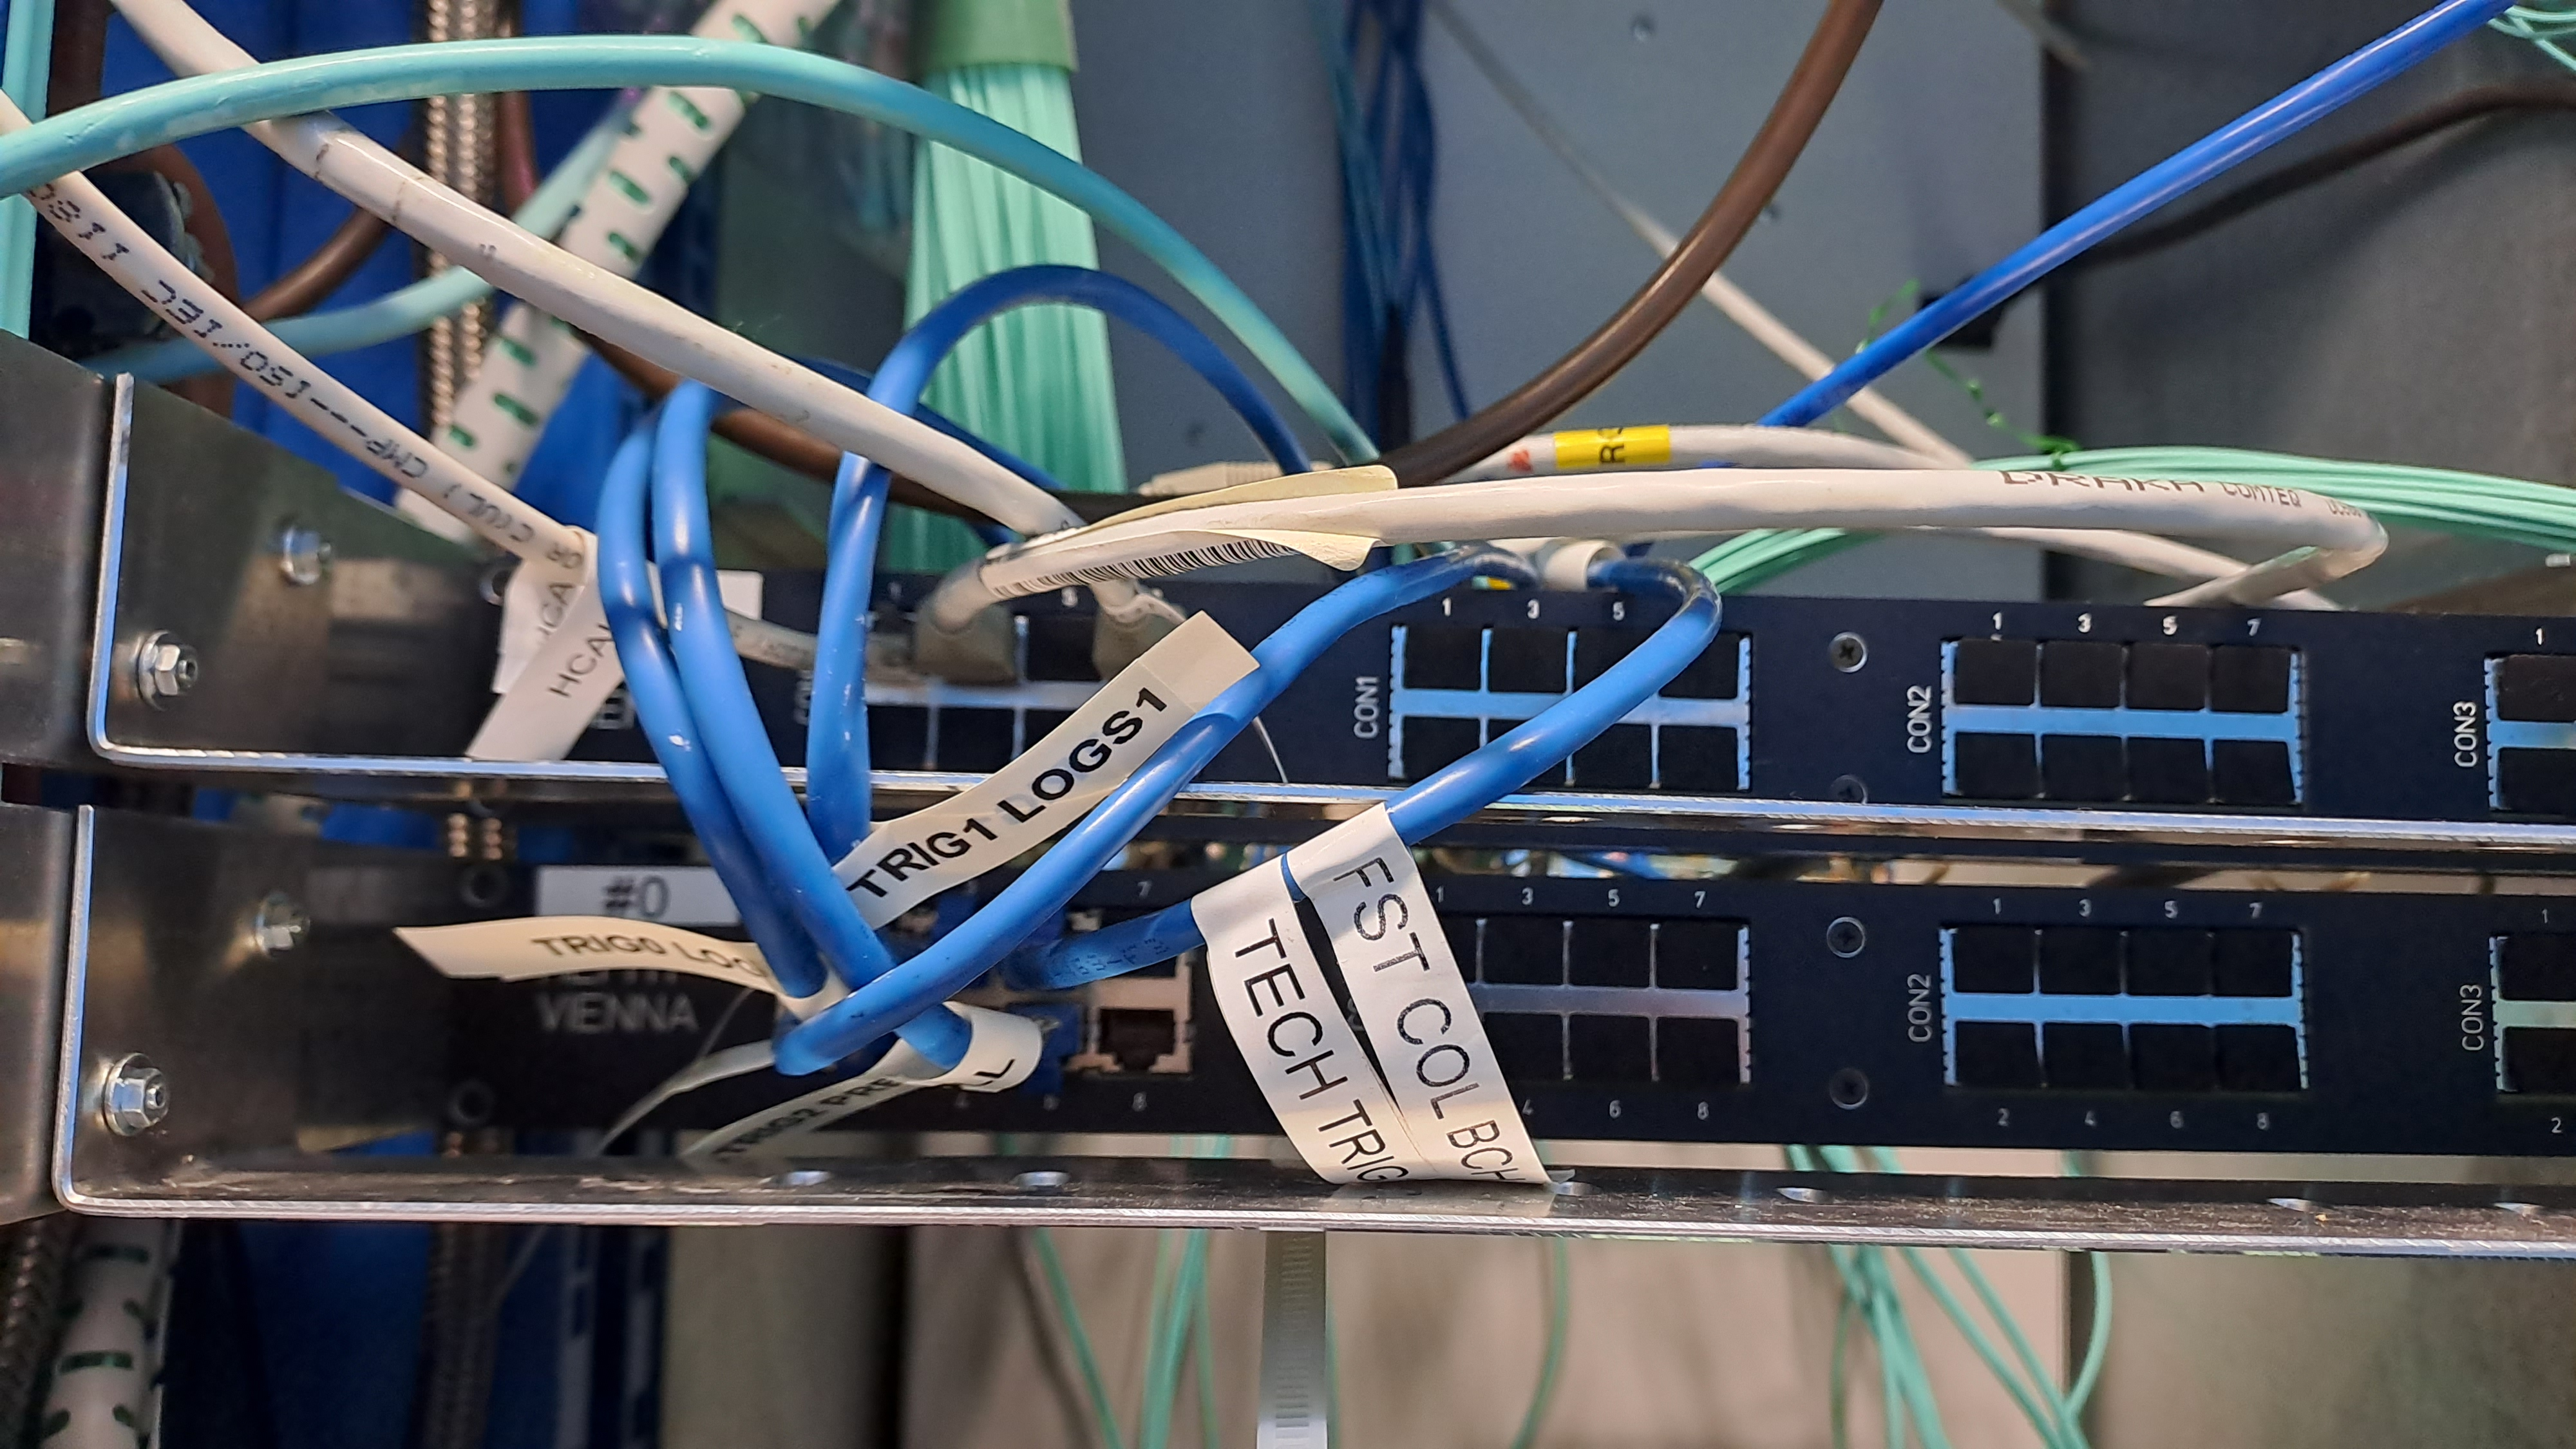
\includegraphics[width=15cm]{figures/ext_cond_pp}
\caption{External condtion patch panel (picture date: September 12, 2023)}
\label{fig:appl:ext_cond_pp}
\end{figure}

\clearpage


    \section{Glossary}\label{sec:glossary}

\begin{description}
\item {\egamma} = electron/gamma objects over Calo-Layer2 (VHDL: eg)
\item {jet} = jet objects over Calo-Layer2 (VHDL: jet)
\item {tau} = tau objects over Calo-Layer2 (VHDL: tau)
\item {muon} = muon objects over \ugmt (VHDL: muon)
\item {\ett} = Scalar sum of transverse energy components over Calo-Layer2 (VHDL: ett)
\item {ETTEM} = Scalar sum of transverse energy components from ECAL only over Calo-Layer2 (VHDL: ettem)
\item {MBTxHFy} = Minimum bias HF bits (VHDL: MBT0HFP, MBT0HFM, MBT1HFP, MBT1HFM)
\item {\htt} = Magnitude of the vectorial sum of transverse energy of jets (hadronic) over Calo-Layer2 (VHDL: htt)
\item {TOWERCOUNT} = tower counts (VHDL: towercount)
\item {\etm} = 2-vector sum of transverse energy over Calo-Layer2 (VHDL: etm)
\item {\htm} = Missing Total transverse energy of jets over Calo-Layer2 (VHDL: htm)
\item {ET$_{miss}^{HF}$} = 2-vector sum of transverse energy including HF over Calo-Layer2 (VHDL: etmhf)
\item {HT$_{miss}^{HF}$} = Missing Total transverse energy of jets including HF over Calo-Layer2 (VHDL: htmhf)
\item {ASYMET} = Asymmetry of ET over Calo-Layer2 (VHDL: asymet)
\item {ASYMHT} = Asymmetry of HT over Calo-Layer2 (VHDL: asymht)
\item {ASYMETHF} = Asymmetry of ET including HF over Calo-Layer2 (VHDL: asymethf)
\item {ASYMHTHF} = Asymmetry of HT including HF over Calo-Layer2 (VHDL: asymhthf)
\item {CENTx} = Centrality bits [7:0] over Calo-Layer2 (VHDL: cent7, cent6, ...)
\item {\pt} = transverse momentum of muon objects(VHDL: pt)
\item {\et} = energy of calorimeter objects (VHDL: et)
\item {$\eta$} = pseudo-rapidity position (VHDL: eta)
\item {$\varphi$} = azimuth angle position (VHDL: phi)
\item {isolation} = isolation information (VHDL: iso)
\item {quality} = quality information (VHDL: qual)
\item {charge} = charge information of muon objects (VHDL: ch)
\item {unconstrained \pt} = transverse momentum of muon objects (VHDL: upt)
\item {impact parameter} = impact parameter information of muon objects (VHDL: ip)
\item {hadronic shower} = hadronic shower (muon shower [mus]) information, on bit 61 of MU0, MU2, MU4 and MU6 (VHDL: mus0, mus1, musoot0, musoot1)
\item {DISP} = displaced bit of jet objects (VHDL: disp)
\item {index bits} = index bits of muon objects - currently not used
\end{description}

\clearpage

    %
%  abbreviation.sty
%
% Repository path : $HeadURL: svn://heros.hephy.at/GlobalTriggerUpgrade/utils/latex/acronyms.sty $
% Last committed : $Revision: 3922 $
% Last changed by : $Author: bergauer $
% Last changed date : $Date: 2015-05-07 08:52:07 +0200 (Thu, 07 May 2015) $
% Description : A reference document for information and explanations of acronyms and common terms in the Global Trigger Group.
%
%% MTCA definition.
\newcommand{\utca}{\ensuremath{\mu\mathrm{TCA}}\xspace}
\newcommand{\utcatech}{\ensuremath{\mu\mathrm{TCA}} Technology \xspace}
\newcommand{\mch}{ MicroTCA~Carrier~Hub \xspace}
\newcommand{\pw}{ \utca ~Power~Module \xspace}
\newcommand{\amc}{AdvancedMC \xspace}
\newcommand{\gbe}{GbE \xspace}
\newcommand{\fmc}{FMC \xspace}
\newcommand{\fpga}{FPGA \xspace}
\newcommand{\pcie}{PCIe \xspace}
\newcommand{\qiq}{QorIQ \xspace}
\newcommand{\cbs}{Cross Bar Switch \xspace}
\newcommand{\gbps}{Gb/s\xspace}


%% GT definition.
\newcommand{\gt}{Global~Trigger\xspace}
\newcommand{\gmt}{Global~Muon~Trigger\xspace}
\newcommand{\tcs}{Trigger~Control~System\xspace}
\newcommand{\gtl}{Global~Trigger~Logic\xspace}
\newcommand{\tim}{Timing~Board\xspace}
\newcommand{\psb}{Pipelined~Synchronizing~Buffer\xspace}
\newcommand{\fdl}{Final~Decision~Logic\xspace}
\newcommand{\rop}{Readout-Process\xspace}
\newcommand{\finor}{Final-OR\xspace}
\newcommand{\record}{Readout-record\xspace}
\newcommand{\serdes}{SerDes\xspace}


%% GT upgrade definition.
\newcommand{\utcs}{\ensuremath{\mu\mathrm{TCS}}\xspace}
\newcommand{\ugtl}{\ensuremath{\mu\mathrm{GTL}}\xspace}
\newcommand{\ufdl}{\ensuremath{\mu\mathrm{FDL}}\xspace}
\newcommand{\ugmt}{\ensuremath{\mu\mathrm{GMT}}\xspace}
\newcommand{\ugt}{\ensuremath{\mu\mathrm{GT}}\xspace}
\newcommand{\ipbus}{IPBus\xspace}

%%GCT
% \newcommand{\gct}{\nohyphens{Global~Calorimeter~Trigger}\xspace}
\newcommand{\gct}{\nohyphens{Calorimeter~Trigger~Layer-2}\xspace}

% Some shorthand
% turn off italics
\newcommand {\etal}{\mbox{et al.}\xspace} %et al. - no preceding comma
\newcommand {\ie}{\mbox{i.e.}\xspace}     %i.e.
\newcommand {\eg}{\mbox{e.g.}\xspace}     %e.g.
\newcommand {\etc}{\mbox{etc.}\xspace}     %etc.
\newcommand {\vs}{\mbox{\sl vs.}\xspace}      %vs.
\newcommand {\mdash}{\ensuremath{\mathrm{-}}} % for use within formulas

% Physics symbols ...

% \newcommand{\PT}{\ensuremath{p_{\mathrm{T}}}\xspace}
% \newcommand{\pt}{\ensuremath{p_{\mathrm{T}}}\xspace}
% \newcommand{\ET}{\ensuremath{E_{\mathrm{T}}}\xspace}
% \newcommand{\et}{\ensuremath{E_{\mathrm{T}}}\xspace}
% \newcommand{\HT}{\ensuremath{H_{\mathrm{T}}}\xspace}
% \newcommand{\Em}{\ensuremath{E\hspace{-0.6em}/}\xspace}
% \newcommand{\Pm}{\ensuremath{p\hspace{-0.5em}/}\xspace}
% \newcommand{\PTm}{\ensuremath{{p}_\mathrm{T}\hspace{-1.02em}/\kern 0.5em}\xspace}
% \newcommand{\PTslash}{\PTm}
% \newcommand{\ETm}{\ensuremath{E_{\mathrm{T}}^{\text{miss}}}\xspace}
% \newcommand{\MET}{\ETm}
% \newcommand{\ETmiss}{\ETm}
% \newcommand{\ETslash}{\ensuremath{E_{\mathrm{T}}\hspace{-1.1em}/\kern0.45em}\xspace}
% \newcommand{\VEtmiss}{\ensuremath{{\vec E}_{\mathrm{T}}^{\text{miss}}}\xspace}
% \newcommand{\elpho}{\ensuremath{\mathrm{e/}\gamma}\xspace} %electron-photon

%% GT upgrade object types
\newcommand{\PT}{\ensuremath{p_{\mathrm{T}}}\xspace}
\newcommand{\pt}{\ensuremath{p_{\mathrm{T}}}\xspace}
\newcommand{\ET}{\ensuremath{E_{\mathrm{T}}}\xspace}
\newcommand{\et}{\ensuremath{E_{\mathrm{T}}}\xspace}
\newcommand{\egamma}{electron/$\gamma$\xspace}
\newcommand{\esums}{energy sum quantities\xspace}
\newcommand{\Egamma}{Electron/$\gamma$\xspace}
\newcommand{\Esums}{Energy sum quantities\xspace}
%\newcommand{\etm}{ETmiss\xspace}
%\newcommand{\htm}{HTmiss\xspace}
\newcommand{\etm}{\ensuremath{ET_{\mathrm{miss}}}\xspace}
\newcommand{\htm}{\ensuremath{HT_{\mathrm{miss}}}\xspace}
\newcommand{\ett}{ET\xspace}
\newcommand{\htt}{HT\xspace}


    % List of tables.
    \doctables{}

    % List of figures.
    \docfigures{}

    % \section*{Acronyms}
    % \begin{acronym}
    % %
%  abbreviation.sty
%
% Repository path : $HeadURL: svn://heros.hephy.at/GlobalTriggerUpgrade/utils/latex/acronyms.sty $
% Last committed : $Revision: 3922 $
% Last changed by : $Author: bergauer $
% Last changed date : $Date: 2015-05-07 08:52:07 +0200 (Thu, 07 May 2015) $
% Description : A reference document for information and explanations of acronyms and common terms in the Global Trigger Group.
%
%% MTCA definition.
\newcommand{\utca}{\ensuremath{\mu\mathrm{TCA}}\xspace}
\newcommand{\utcatech}{\ensuremath{\mu\mathrm{TCA}} Technology \xspace}
\newcommand{\mch}{ MicroTCA~Carrier~Hub \xspace}
\newcommand{\pw}{ \utca ~Power~Module \xspace}
\newcommand{\amc}{AdvancedMC \xspace}
\newcommand{\gbe}{GbE \xspace}
\newcommand{\fmc}{FMC \xspace}
\newcommand{\fpga}{FPGA \xspace}
\newcommand{\pcie}{PCIe \xspace}
\newcommand{\qiq}{QorIQ \xspace}
\newcommand{\cbs}{Cross Bar Switch \xspace}
\newcommand{\gbps}{Gb/s\xspace}


%% GT definition.
\newcommand{\gt}{Global~Trigger\xspace}
\newcommand{\gmt}{Global~Muon~Trigger\xspace}
\newcommand{\tcs}{Trigger~Control~System\xspace}
\newcommand{\gtl}{Global~Trigger~Logic\xspace}
\newcommand{\tim}{Timing~Board\xspace}
\newcommand{\psb}{Pipelined~Synchronizing~Buffer\xspace}
\newcommand{\fdl}{Final~Decision~Logic\xspace}
\newcommand{\rop}{Readout-Process\xspace}
\newcommand{\finor}{Final-OR\xspace}
\newcommand{\record}{Readout-record\xspace}
\newcommand{\serdes}{SerDes\xspace}


%% GT upgrade definition.
\newcommand{\utcs}{\ensuremath{\mu\mathrm{TCS}}\xspace}
\newcommand{\ugtl}{\ensuremath{\mu\mathrm{GTL}}\xspace}
\newcommand{\ufdl}{\ensuremath{\mu\mathrm{FDL}}\xspace}
\newcommand{\ugmt}{\ensuremath{\mu\mathrm{GMT}}\xspace}
\newcommand{\ugt}{\ensuremath{\mu\mathrm{GT}}\xspace}
\newcommand{\ipbus}{IPBus\xspace}

%%GCT
% \newcommand{\gct}{\nohyphens{Global~Calorimeter~Trigger}\xspace}
\newcommand{\gct}{\nohyphens{Calorimeter~Trigger~Layer-2}\xspace}

% Some shorthand
% turn off italics
\newcommand {\etal}{\mbox{et al.}\xspace} %et al. - no preceding comma
\newcommand {\ie}{\mbox{i.e.}\xspace}     %i.e.
\newcommand {\eg}{\mbox{e.g.}\xspace}     %e.g.
\newcommand {\etc}{\mbox{etc.}\xspace}     %etc.
\newcommand {\vs}{\mbox{\sl vs.}\xspace}      %vs.
\newcommand {\mdash}{\ensuremath{\mathrm{-}}} % for use within formulas

% Physics symbols ...

% \newcommand{\PT}{\ensuremath{p_{\mathrm{T}}}\xspace}
% \newcommand{\pt}{\ensuremath{p_{\mathrm{T}}}\xspace}
% \newcommand{\ET}{\ensuremath{E_{\mathrm{T}}}\xspace}
% \newcommand{\et}{\ensuremath{E_{\mathrm{T}}}\xspace}
% \newcommand{\HT}{\ensuremath{H_{\mathrm{T}}}\xspace}
% \newcommand{\Em}{\ensuremath{E\hspace{-0.6em}/}\xspace}
% \newcommand{\Pm}{\ensuremath{p\hspace{-0.5em}/}\xspace}
% \newcommand{\PTm}{\ensuremath{{p}_\mathrm{T}\hspace{-1.02em}/\kern 0.5em}\xspace}
% \newcommand{\PTslash}{\PTm}
% \newcommand{\ETm}{\ensuremath{E_{\mathrm{T}}^{\text{miss}}}\xspace}
% \newcommand{\MET}{\ETm}
% \newcommand{\ETmiss}{\ETm}
% \newcommand{\ETslash}{\ensuremath{E_{\mathrm{T}}\hspace{-1.1em}/\kern0.45em}\xspace}
% \newcommand{\VEtmiss}{\ensuremath{{\vec E}_{\mathrm{T}}^{\text{miss}}}\xspace}
% \newcommand{\elpho}{\ensuremath{\mathrm{e/}\gamma}\xspace} %electron-photon

%% GT upgrade object types
\newcommand{\PT}{\ensuremath{p_{\mathrm{T}}}\xspace}
\newcommand{\pt}{\ensuremath{p_{\mathrm{T}}}\xspace}
\newcommand{\ET}{\ensuremath{E_{\mathrm{T}}}\xspace}
\newcommand{\et}{\ensuremath{E_{\mathrm{T}}}\xspace}
\newcommand{\egamma}{electron/$\gamma$\xspace}
\newcommand{\esums}{energy sum quantities\xspace}
\newcommand{\Egamma}{Electron/$\gamma$\xspace}
\newcommand{\Esums}{Energy sum quantities\xspace}
%\newcommand{\etm}{ETmiss\xspace}
%\newcommand{\htm}{HTmiss\xspace}
\newcommand{\etm}{\ensuremath{ET_{\mathrm{miss}}}\xspace}
\newcommand{\htm}{\ensuremath{HT_{\mathrm{miss}}}\xspace}
\newcommand{\ett}{ET\xspace}
\newcommand{\htt}{HT\xspace}

    % \end{acronym}

    \clearpage

    \begin{thebibliography}{00}

    \bibitem {MP7}
    MP7 documentation:\\
    \url{http://www.hep.ph.ic.ac.uk/mp7}

    \bibitem {MP7 firmware}
    MP7 firmware repository (GitLab account reqired):\\
    \url{https://gitlab.cern.ch/cms-cactus/firmware/mp7}

    \bibitem {Virtex7}
    Xilinx Series 7 overview:\\
    \url{https://docs.xilinx.com/v/u/en-US/ds180_7Series_Overview}

    \bibitem {interface}
    Calo-layer2 and Global Muon Trigger interface documentation:\\
    \url{https://raw.githubusercontent.com/cms-l1-globaltrigger/mp7_ugt_legacy/master/doc/scales_inputs_2_ugt/pdf/scales_inputs_2_ugt.pdf}

    \bibitem {TME_repo}
    Trigger Menu Editor repository:\\
    \url{https://github.com/cms-l1-globaltrigger/tm-editor}

    \bibitem {VHDL_Producer}
    VHDL Producer repository:\\
    \url{https://github.com/cms-l1-globaltrigger/tm-vhdlproducer}

    \bibitem {GTHs}
    Xilinx Series 7 Transceivers (GTHs) documentation:\\
    \url{https://www.xilinx.com/support/documentation/user_guides/ug476_7Series_Transceivers.pdf}

    \end{thebibliography}

% End of document structure.
\end{document}

% eof
